\documentclass[../main.tex]{subfiles}
\usepackage{slashed}
\usepackage[table]{xcolor}
\usepackage{hhline}
\usepackage{lipsum}

\let\Bbbk\relax
\usepackage{amsmath}
\usepackage{amsfonts}
\usepackage{simpler-wick}

\begin{document}
\setchapterimage[6.5cm]{images_ch5/hiding_infinities.png}
\setchapterpreamble[u]{\margintoc}
\chapter[Conseguenze della Rinormalizzazione]{Conseguenze della Rinormalizzazione\footnote{Immagine da \href{https://youtu.be/0OQ7BhlfAJY}{Renormalization: The Art of Erasing Infinity}.}}
\labch{ren_conseq}
\fboxsep =1pt % separazione per i box

\section{Il potenziale Coulombiano}
Consideriamo lo scattering di un elettrone in presenza di un potenziale elettromagnetico esterno, per esempio generato da un nucleo pesante, all'ordine minore in teoria delle perturbazioni.

\[
\feynmandiagram[vertical'=a to b] {
                                        i1[particle=\(e^-\)] -- [fermion, edge label=\(p\)] a[dot] -- [fermion, edge label=\(p'\)] i2[particle=\(e^-\)],
                                        b[large, crossed dot, label=below:\(Ze\)] -- [photon, momentum'=\(q\)] a
                                        };
\]

La transizione considerata può essere formalizzata come una transizione \(|i\rangle \rightarrow |f\rangle \) dove:
\[
|i\rangle = |e^-(p,r)\rangle ~~,~~ |f\rangle = |e^-(p',s)\rangle
\]
con $r$ ed $s$ stati di polarizzazione.

L'idea del procedimento che adotteremo è la seguente: 
\begin{enumerate}
    \item Calcoliamo l'ampiezza in QED;
    \item Ragioniamo sulla struttura del potenziale esterno utilizzando la teoria classica dei campi;
    \item Prendiamo il limite non relativistico dell'ampiezza in QED;
    \item Considerando lo scattering di un autostato di impulso in presenza di un potenziale $V(\Vec{x})$, i.e. il processo \(|\Vec{p}\rangle \rightarrow |\Vec{p}'\rangle \), lo valutiamo con un calcolo di meccanica quantistica e compariamo con il risultato del punto 3.
\end{enumerate}

\begin{enumerate}
    \item[\textbf{1)}] \textbf{Ampiezza in QED} \\
    Nel termine di interazione \(\mathscr{L}_{int}=e\bar\psi\gamma^\mu A_\mu\psi\) consideriamo il campo $A_\mu(x)$ come un campo classico, ossia esterno. Inoltre lo consideriamo statico, i.e. indipendente dal tempo: \(A_\mu(x)\rightarrow A^\text{ext}_\mu(\Vec x)\).

    Al tree-level il calcolo dell'ampiezza di scattering consiste nel calcolo di
    \begin{equation}
        S_{fi} = (ie)\int d^4x\, \wick[positions={+1,-1}]{\c1{\langle e^-(p',s)|} \c1{\bar\psi}\gamma^\mu \c2{\psi} \c2{|e^-(p,r)\rangle}} A^\text{ext}_\mu(\Vec x)
        \label{eq:coulomb_scattering_amplitude_QED_init}
    \end{equation}
    \begin{nota}
        Stiamo considerando un campo di Dirac con la normalizzazione non relativistica:
        \begin{align*}
            \psi = \int \frac{d^3\Vec{k}}{(2\pi^3)} \sqrt{\frac{m}{E_k}} \sum_\alpha\Bigl[ a(\Vec k,\alpha)u(k,\alpha)e^{-ik\cdot x} + b^\dagger(\Vec k,\alpha)v(k,\alpha)e^{ik\cdot x} \Bigr] \\
            \bar\psi = \int \frac{d^3\Vec{k}}{(2\pi^3)} \sqrt{\frac{m}{E_k}} \sum_\alpha\Bigl[ a^\dagger(\Vec k,\alpha)\bar u(k,\alpha)e^{ik\cdot x} + b(\Vec k,\alpha)\bar v(k,\alpha)e^{-ik\cdot x} \Bigr]
        \end{align*}
        da cui definiamo:
        \begin{align*}
            &|e^-(\Vec p, s)\rangle = \sqrt{\frac{E_p}{m}}a^\dagger(\Vec p, s)|0\rangle \\
            &\bigl[a(\Vec p, r),a^\dagger(\Vec q, s) \bigr]_+ = (2\pi)^3\delta(\Vec p - \Vec q)\delta_{rs}\\
            &\langle e^-(q, s)|e^-(\Vec p, r)\rangle = \sqrt{\frac{E_q}{m}}\sqrt{\frac{E_p}{m}}(2\pi)^3\delta(\Vec p - \Vec q)\delta_{rs}
        \end{align*}
        Qui bisogna scegliere una convenzione da seguire per dare un senso coerente ai campi $\psi$ e $\bar\psi$. In sostanza va scelto se procedere con l'obiettivo di arrivare a \(\langle 0|0\rangle = 1\), lavorando solamente sul bra o solamente sul ket (creando e successivamente distruggendo distruggendo), oppure con l'obiettivo di arrivare a \(\langle e^-|e^-\rangle = 1\), lavorando simultaneamente su bra e ket.
        
        Personalmente, sono un fan della prima, quindi al campo $\psi$ associamo l'operazione di distruzione di particella e creazione di antiparticella quando agente \textbf{sul ket}, mentre al campo $\bar\psi$ associamo l'opposto: creazione di particella e distruzione di antiparticella quando agente \textbf{sul ket}. Ovviamente vale l'opposto se si agisce sul bra.
        \label{note:creation_destruction_convention}
    \end{nota}

    Scriviamo allora:
    \[
    \begin{aligned}
    S_{fi} &= (ie)\int d^4x\, \langle 0|\sqrt{\frac{E_p'}{m}} a(\Vec p',s) \bar\psi\gamma^\mu \psi \sqrt{\frac{E_p}{m}} a^\dagger(\Vec p,r)|0\rangle A^\text{ext}_\mu(\Vec x) \\
    & 
        \begin{aligned}
            =&(ie)\sqrt{\frac{E_p'}{m}}\sqrt{\frac{E_p}{m}}\int d^4x\int \frac{d^3\Vec k}{(2\pi)^3}\int \frac{d^3\Vec k'}{(2\pi)^3}\,\sqrt{\frac{m}{E_k}}\sqrt{\frac{m}{E_{k'}}} \sum_\alpha\sum_\beta\\
            &\times \langle 0| a(\Vec p',s)a^\dagger(\Vec k,\alpha)\bar u( k,\alpha)e^{ik\cdot x} \gamma^\mu a(\Vec k',\beta) u( k',\beta)e^{-ik'\cdot x} a^\dagger(\Vec p,r)|0\rangle A^\text{ext}_\mu(\Vec x) \overset{\star}{=}
        \end{aligned}
    \end{aligned}
    \]
    Ora concentriamoci sul sandwich ed applichiamo le relazioni di anti-commutazione agli operatori $a$, ricordando che $a|0\rangle = 0$, $\langle 0 | a^\dagger =0$ e $\langle 0|0\rangle = 1$ abbiamo:
    \[
    (2\pi)^3\delta(\Vec p' - \Vec k)\delta_{s\alpha}(2\pi)^3\delta(\Vec p - \Vec k')\delta_{\beta r} \, \bar u( k,\alpha) \gamma^\mu u( k',\beta) \,e^{ik\cdot x-ik'\cdot x}
    \]
    Possiamo quindi sfruttare le $\delta$ per svolgere i due integrali 3D e togliere di mezzo le \(\sqrt{\frac{E}{m}}\sqrt{\frac{m}{E}}\) forzando $k = p'$ e $k'=p$. Otteniamo quindi:

    \begin{align*}
       &\overset{\star}{=} (ie)\int d^4x\, \bar u( p',\alpha) \gamma^\mu u( p,\beta) \,e^{ip'\cdot x-ip\cdot x}A^\text{ext}_\mu(\Vec x)\\
       &=(ie) 
       \underbrace{\int dt\,\bigl[e^{i(E_{p'}-E_p)t}\bigr]}_{=2\pi \delta(E_{p'}-E_p)}
       \bar u( p',\alpha) \gamma^\mu u( p,\beta) 
       \underbrace{\int d^3\Vec x\,\bigl[e^{-i(\Vec p'-\Vec p)\cdot\Vec x}A^\text{ext}_\mu(\Vec x)\bigr]}_{=\Tilde{A}_\mu^\text{ext}(\Vec{q} = \Vec p'-\Vec p)}
    \end{align*}
    Siamo quindi pronti a scrivere il risultato finale, sfruttando la riscrittura di \(A^\text{ext}_\mu(\Vec x)\) dello spazio dell'impulso tramite la sua trasformata di Fourier:
    \begin{equation}
    \boxed{
        S_{fi}=(2\pi) \delta(E_{p'}-E_p) (ie)\bar u(p',\alpha) \gamma^\mu u( p,\beta)\Tilde{A}_\mu^\text{ext}(\Vec{q})
        }
        \label{eq:coulomb_scattering_amplitude_QED_final}
    \end{equation}
    \textbf{Commento:} abbiamo solo la conservazione dell'energia, mentre l'impulso spaziale non si conserva: difatti avviene un trasferimento di impulso $\Vec{q} = \Vec p'-\Vec p$ dall'elettrone al nucleo.

    \item[\textbf{2)}] \textbf{Il campo classico esterno} \\
    Concentriamoci su $A^\text{ext}_\mu(\Vec x)$ ed utilizziamo la teoria dei campi classica.
    La Lagrangiana è:
    \[
    \mathscr L = -\frac{1}{4}F_{\mu\nu}F^{\mu\nu} - A_\mu j^\mu
    \]
    con \(j^\mu\) sorgente esterna associata al nucleo pesante.

    Da questa Lagrangiana si derivano le le equazioni del moto di Eulero-Lagrange:
    \[
    \partial_\mu F^{\mu\nu} = j^\nu
    \]
    identificate con le equazioni di Maxwell in presenza di una sorgente.

    In termini di $A_\mu$ possiamo scrivere:
    \begin{align*}
        \partial_\mu \bigl(\partial^\mu A^\nu - \partial^\nu A^\mu\bigr) &= \Box A^\nu - \underbrace{\cancel{\partial^\nu\bigl(\partial_\mu A^\mu\bigr)}}_{\substack{\text{Gauge di Lorentz}\\ \partial_\mu A^\mu = 0}} = j^\nu \\
        &\Rightarrow \boxed{\Box A^\mu = j^\mu}
    \end{align*}

    Ricordando l'assunzione di staticità del potenziale, che si traduce in \(\partial_t A^\mu = 0\) riduce il D'Alembertiano al solo Laplaciano \[\Box = \partial_t^2 - \nabla^2 \rightarrow -\nabla^2 = -\Delta\]
    Le equazioni del moto in assunzione di campo statico diventano quindi:
    \begin{equation}
        \Delta A^\mu(\Vec x) = -j^\mu(\Vec x)
        \label{eq:static_maxwell_eq_source}
    \end{equation}
    Possiamo parametrizzare $j^\mu$ pensandola come una corrente generata da una carica $Ze$ posta a riposo nell'origine: \marginnote{Essendo la carica a riposo, la 3-corrente sarà nulla.}
    \[
    j^\mu(\Vec x) = 
    \begin{cases} 
        j^0(\Vec{x}) = Ze\delta(\Vec x)\\
        j^i(\Vec{x}) = 0
    \end{cases}
    \]
    Le nostre equazioni del moto si riducono quindi all'equazione:
    \[
    \Delta A^0(\Vec x) = -Ze\delta(\Vec{x})
    \]
    In quanto le tre componenti spaziali del potenziale, data la struttura della corrente, possono essere messe a zero senza alcuna perdita di generalità.

    Per trovare la soluzione per la componente temporale, lavoriamo nello spazio di Fourier, adoperando le seguenti sostituzioni:
    \[
    A^\mu(\Vec x) = \int\frac{d^3\Vec q}{(2\pi)^3}\Tilde{A}^\mu(\Vec{q})e^{i\Vec{q}\cdot\Vec{x}} ~~,~~ \delta(\Vec{x}) = \int\frac{d^3\Vec q}{(2\pi)^3}e^{i\Vec{q}\cdot\Vec{x}} 
    \]
    L'azione del Laplaciano sul potenziale “tira giù” un fattore $-|\Vec{q}|^2$ dall'esponenziale e risolvendo per $\Tilde A^0(\Vec q)$ troviamo: 
    \[ \Tilde A^0(\Vec q) = \frac{Ze}{|\Vec{q}|^2}\]

    Riscriviamo allora l'ampiezza:
    \begin{equation}
    \boxed{
        \begin{aligned}
        S_{fi}&=(2\pi) \delta(E_{p'}-E_p) (ie)\bar u(p',\alpha) \gamma^\mu u( p,\beta)\Tilde{A}_\mu^\text{ext}(\Vec{q})\\
        & \Tilde A^0(\Vec q) = \frac{Ze}{|\Vec{q}|^2} ~~,~~ A^i=0 
        \end{aligned}
        }
        \label{eq:coulomb_scattering_amplitude_QED_with_potential}
    \end{equation}

    \item[\textbf{3)}] \textbf{Limite non relativistico dell'ampiezza in QED}\\
    Adottando la rappresentazione di Dirac per le matrici $\gamma$
    \[
    \gamma^0 = 
    \begin{pmatrix} 
    \mathbb 1 &          0\\
            0 & -\mathbb 1
    \end{pmatrix} ~~,~~
    \gamma^i = 
    \begin{pmatrix} 
            0 &   \sigma^i\\
    -\sigma^i &          0
    \end{pmatrix}
    \]
    scriviamo esplicitamente gli spinori di Dirac, ovvero le soluzioni dell'equazione di Dirac libera in questa rappresentazione:
    \[
    u(p,s) = N
    \begin{pmatrix} 
        \chi(s) \\
        \frac{\Vec\sigma\cdot \Vec p}{E+m}\chi(s)
    \end{pmatrix}
    \]
    con $\chi(s)$ autostato di spin bi-dimensionale (i.e. la polarizzazione).
    \begin{nota}
        Nella convenzione che stiamo utilizzando in questa sezione, gli spinori sono normalizzati secondo la seguente relazione:
        \begin{equation}
            u^\dagger(p,s)u(p,r) = \delta_{sr}\frac{E_p}{m}
            \label{eq:spinor_normalization}
        \end{equation}
        Di conseguenza possiamo definire la soluzione in onde piane e il prodotto scalare tra due soluzioni di questo tipo, rispettivamente:
        \begin{align*}
            &\psi_{\Vec{p}}^{(s)} = \sqrt{\frac{m}{E_p}} u(p,s)e^{-ip\cdot x}\\ 
            \int d^3x \, &{\psi_{\Vec{p}}^{(s)}}^\dagger(x) \psi_{\Vec{p}'}^{(r)}(x) = (2\pi)^3\delta_{sr}\delta(\Vec{p}-\Vec p')
        \end{align*}
        Allo stesso tempo, considerando 
        \[ \hat\psi(x) = \int\frac{d^3\Vec{k}}{(2\pi)^3}\sqrt\frac{m}{E_k}\sum_\alpha a(\Vec k,\alpha)u(k,\alpha)e^{-ik\cdot x} 
        \]
        possiamo esprimere gli operatori di creazione e distruzione come segue:
        \begin{align*}
            &a(\Vec{p},s) = \int d^3\Vec{x} \, {\psi_{\Vec{p}}^{(s)}}^\dagger(x)\hat\psi(x)\\
            &a^\dagger(\Vec{p},s) = \int d^3\Vec{x} \, {\psi_{\Vec{p}}^{(s)}}(x)\hat\psi^\dagger(x)
        \end{align*}

        tra cui vale la relazione di anti-commutazione:
        \[
        \Big[ a(\Vec{p},s), ~a^\dagger(\Vec{p}',r) \Big]_+ = (2\pi)^3\delta_{sr}\delta(\Vec{p} - \Vec{p}')
        \]
    \end{nota}
    
    Partendo dalla (\ref{eq:spinor_normalization}), sostituendo l'espressione degli spinori e svolgendo i calcoli, è possibile trovare la struttura esplicita di $N$. Si trova infatti:
    \[
    N = \bigg( \frac{E+m}{2m} \bigg)^{\nicefrac{1}{2}}
    \]
    Per cui sostituendo nell'espressione generica per gli spinori di Dirac:

    \begin{equation}
        \boxed{
        u(p,s) = \bigg( \frac{E+m}{2m} \bigg)^{\nicefrac{1}{2}}
        \begin{pmatrix} 
            \chi(s) \\
            \frac{\Vec\sigma\cdot \Vec p}{E+m}\chi(s)
        \end{pmatrix}}
        \label{eq:spinor_structure_normalized}
    \end{equation}

    Consideriamo ora il limite non relativistico \(|\Vec{p}| \ll m \Rightarrow \nicefrac{|\Vec{p}|}{m} \ll 1\) e diciamo che vogliamo tenere fino all'ordine $\mathscr{O}\big(\nicefrac{|\Vec{p}|}{m}\big)$. Di conseguenza espandendo l'energia otteniamo:
    \[
    E = \big(p^2 + m^2\big)^{\nicefrac{1}{2}} = m \Big( 1 + \frac{p^2}{m^2}\Big)^{\nicefrac{1}{2}} \approx m\Big[1 + \frac{1}{2}\frac{p^2}{m^2} + \mathscr{O}\Big(\frac{p^4}{m^4}\Big) \Big]
    \]
    Quindi, nel limite non relativistico all'ordine inferiore:
    \[
    \boxed{p^\mu = (m,~ \Vec p)~~,~~p'^\mu = (m,~ \Vec p')}
    \]

    Ma allora, se torniamo alla (\ref{eq:coulomb_scattering_amplitude_QED_with_potential}) e tralasciamo la parte spaziale possiamo calcolare esplicitamente:
    \begin{align*}
        \bar u(p',\, \alpha) \gamma^0 u(p,\, \beta) &= u^\dagger(p',\, \alpha) (\gamma^0)^2 u(p,\, \beta) =\\
        &= \chi^\dagger(\alpha)\chi(\beta) + \frac{1}{4m^2}\chi^\dagger(\alpha) ~\Vec{\sigma}\cdot\Vec{p}'~\Vec{\sigma}\cdot\Vec{p}~\chi(\beta)\\
        & = \delta_{\alpha\beta} + \mathscr{O}\Big(\frac{p^2}{m^2}\Big) = \delta_{\alpha\beta}
    \end{align*}
    
    Arriviamo quindi a
    \begin{equation}
        \boxed{S_{fi} \overset{\text{NR}}{=} (2\pi) \delta(E_{p'} - E_p) (ie) \delta_{\alpha\beta} \frac{Ze}{|\Vec q|^2}}
        \label{eq:coulomb_scattering_amplitude_QED_NR}
    \end{equation}

    \item[\textbf{4)}] \textbf{Comparazione con il calcolo in meccanica quantistica}\\ 
    Calcoliamo l'ampiezza di scattering per un autostato di impulso $\Vec p$ in presenza di un potenziale statico, utilizzando lo schema di interazione in meccanica quantistica.
    \begin{align*}
        A\Big( |\Vec{p}\rangle \rightarrow |\Vec{p}'\rangle\Big) &= \langle \Vec{p}'|U_I(+\infty, -\infty)|\Vec{p}\rangle \\
        &=\langle \Vec{p}'| \Big[\mathbb 1 - i\int\limits_{-\infty}^{+\infty}dt\, \hat V^{(I)}_{int}(t)\Big]|\Vec{p}\rangle
    \end{align*}
    con \(\hat V^{(I)}_{int}(t) = e^{iH_0t}\hat V_{int}e^{-iH_0t}\).

    La parte connessa dell'ampiezza è \marginnote{qui utilizziamo il fatto che $|\Vec{p}\rangle$ è autostato di impulso, il che si traduce nell'equazione agli autovalori \(e^{-iH_0t}|\Vec{p}\rangle = e^{-iE_pt}|\Vec{p}\rangle\).}
    \begin{align*}
        A\Big( |\Vec{p}\rangle \rightarrow |\Vec{p}'\rangle\Big) &= - i\langle \Vec{p}'|\int\limits_{-\infty}^{+\infty}dt\, e^{iH_0t}\hat V_{int}e^{-iH_0t}|\Vec{p}\rangle \\
        & =  - i\int\limits_{-\infty}^{+\infty}dt\, e^{iE_{p'}t}e^{-iE_pt} 
            \underbrace{\langle \Vec{p}'| \hat V_{int} |\Vec{p}\rangle}_{\substack{\text{non dipende}\\\text{da t}}}\\
        & = -i(2\pi)\delta(\Vec{p}' - \Vec{p})\langle \Vec{p}'| \hat V_{int} |\Vec{p}\rangle
    \end{align*}
    comparando con la (\ref{eq:coulomb_scattering_amplitude_QED_NR}) troviamo immediatamente il \textbf{potenziale nello spazio dell'impulso}:
    \begin{equation}
        \boxed{\langle \Vec{p}'| \hat V_{int} |\Vec{p}\rangle = -\frac{Ze^2}{|\Vec{q}|^2}} ~~,~~ \text{con }\Vec{q} = \Vec{p}' - \Vec{p}
        \label{eq:potential_in_momentum_space}
    \end{equation}
    L'equazione (\ref{eq:potential_in_momentum_space}) ci dice che il limite non relativistico dello scattering Coulombiano in QED fornisce esattamente (e com'è giusto che sia) il potenziale di Coulomb attrattivo. Volendo, questo risultato può essere riportato nello spazio delle posizioni, ma tale operazione è lasciata come esercizio.
\end{enumerate}

\begin{exercise}
    Calcolare il potenziale nello spazio delle posizioni partendo dalla (\ref{eq:potential_in_momentum_space}), per mezzo delle trasformate di Fourier.

    \paragraph{Soluzione.} [\textbf{Conti svolti Lezione 14 pag.10}]
    \begin{equation}
        V(\Vec{x}) = \frac{-Ze^2}{4\pi|\Vec{x|}}
        \label{eq:coulomb_potential}
    \end{equation}
\end{exercise}

\section{Potenziale Coulombiano oltre il tree-level}

Andiamo oltre il calcolo al tree-level, mantenendo l'assunzione di potenziale statico, ma restando generici in merito alla struttura della corrente.

Nello spazio di Fourier abbiamo
\[
A^\mu(\Vec x) = \int\frac{d^3\Vec q}{(2\pi)^3}\Tilde{A}^\mu(\Vec{q})e^{i\Vec{q}\cdot\Vec{x}}~~,~~
j^\mu(\Vec x) = \int\frac{d^3\Vec q}{(2\pi)^3}\Tilde{j}^\mu(\Vec{q})e^{i\Vec{q}\cdot\Vec{x}}
\]

Sostituendo nelle equazioni del moto (\ref{eq:static_maxwell_eq_source}) troviamo:
\[
\int\frac{d^3\Vec q}{(2\pi)^3}\Big[-|\Vec q|^2\Tilde{A}^\mu(\Vec{q}) + \Tilde{j}^\mu(\Vec{q}) \Big]e^{i\Vec{q}\cdot\Vec{x}} = 0 \Rightarrow \boxed{\Tilde{j}^\mu(\Vec{q}) = |\Vec q|^2\Tilde{A}^\mu(\Vec{q})}
\]
Possiamo sostituire \(\Tilde{A}^\mu(\Vec{q})\) nell'ampiezza (\ref{eq:coulomb_scattering_amplitude_QED_final}) ottenendo:

\[
S_{fi}=(2\pi) \delta(E_{p'}-E_p) (ie)\bar u(p',\alpha) \gamma^\mu u( p,\beta)\frac{1}{|\Vec q|^2}\Tilde{j}_\mu(\Vec{q})
\]

Abbiamo già notato come sia conservata l'energia, ma non l'impulso. Volendo riscrivere il trasferimento di impulso per mezzo del suo quadrivettore, ricordiamo che \(q = p'-p\), da cui segue
\[
q^2 = \cancel{(E_{p'} - E_p)^2} - |\Vec{p}' -\Vec{p}|^2 = -|\Vec{q}|^2 \Rightarrow |\Vec{q}|^2 = -q^2
\]

In definitiva scriviamo allora nuovamente la nostra ampiezza, inserendo un $i\cdot(-i) = 1$ e portando l'indice della corrente in alto per mezzo di un tensore metrico, così da dare un senso fisico alla struttura ottenuta:

\begin{equation}
    S_{fi}=(2\pi) \delta(E_{p'}-E_p) 
    \underbrace{\textcolor{Green}{\Big[\bar u(p', \,\alpha) (ie\gamma^\mu) u(p, \,\beta)\Big]}}_{\text{corrente elettronica}}
    \underbrace{\textcolor{Blue}{\frac{-ig_{\mu\nu}}{q^2}}}_{\substack{\text{propagatore}\\\text{fotonico}}}
    \underbrace{\textcolor{Red}{\big(-i\Tilde{j}_\nu(\Vec{q})\big)}}_{\substack{\text{corrente}\\\text{elettromagnetica}\\\text{del secondo}\\\text{vertice}}}
    \label{eq:coulomb_scattering_amplitude_QED_tree}
\end{equation}

dal punto di vista diagrammatico:
\[
\begin{tikzpicture}
    \begin{feynman}
        \diagram[vertical'=a to b] {
            i1 -- [fermion, edge label=\(p\), Green] a[dot, Green] -- [fermion, edge label=\(p'\), Green] i2,
            b[large, crossed dot, Red] -- [photon, momentum'=\(q\), Blue] a
            };
    \end{feynman}
        \draw [decoration={brace}, decorate] ([xshift=.2cm,yshift=-.0cm]i2.north east) -- ([xshift=1.8cm,yshift=-.3cm]a.south east) node [pos=.5, right] {\(\bar u (ie\gamma^\mu) u\)};
        \draw [decoration={brace, mirror}, decorate] ([xshift=-.2cm,yshift=-.0cm]a.west) -- ([xshift=-.2cm,yshift=.2cm]b.west) node [pos=.5, left] {\(\frac{-ig_{\mu\nu}}{q^2}\)};
        \draw [decoration={brace}, decorate] ([xshift=.2cm,yshift=-.0cm]b.north east) -- ([xshift=.2cm,yshift=.0cm]b.south east) node [pos=.5, right] {\(-i\Tilde{j}_\nu(\Vec{q})\)};
\end{tikzpicture}
\]

Comparando con il precedente risultato, arriviamo alla conclusione che il propagatore del fotone sia il responsabile per la presenza del potenziale di Coulomb (in quanto è da lui che arriva la dipendenza da $q^{-2}$).

\subsection{Correzioni al loop sul propagatore del fotone}
Consideriamo i seguenti diagrammi utilizzando il formalismo introdotto nel capitolo precedente, ovvero separando la Lagrangiana in \(\mathscr{L}_R + \mathscr{L}_{ct}\):

\[
\feynmandiagram[horizontal'=a to b, inline=(a.base)] {
    i1 -- [anti fermion, edge label=\(p'\)] a[dot] -- [anti fermion, edge label=\(p\)] i2,
    b[large, crossed dot] -- [photon, momentum'=\(q\)] a
    };
+
\feynmandiagram[horizontal'= d to b, inline=(a.base)] {
    i1 -- [anti fermion, edge label=\(p'\)] a[dot, label=below:$\mu$] -- [anti fermion, edge label=\(p\)] i2,
    a --[photon] c[dot, label=below left:$\rho$] --[fermion, half left] d[dot, label=below right:$\sigma$] --[photon] b[large, crossed dot, label=below:$\nu$],
    d --[fermion, half left] c,
    };
+
\feynmandiagram[horizontal'= c to b, inline=(a.base)] {
    i1 -- [anti fermion, edge label=\(p'\)] a[dot] -- [anti fermion, edge label
    =\(p\)] i2,
    a --[photon] c[small, crossed dot] --[photon] b[large, crossed dot],
    };
\]
Ricordando l'equazione (\ref{eq:corrected_photon_propagator_1loop}), possiamo scrivere l'ampiezza “corretta”\footnote{Nel senso di “rinormalizzata”, se vogliamo.}, sommando all'ampiezza riportata in equazione (\ref{eq:coulomb_scattering_amplitude_QED_tree}), che corrisponde al diagramma al tree-level, i contributi del diagramma al loop e relativo controtermine. \marginnote{Ricordiamo che \textcolor{blue}{possiamo trascurare i termini in \(q^\mu q^\nu\)} per ragioni connesse all'identità di Ward.}

\begin{align*}
S_{fi} = &(2\pi) \delta(E_{p'}-E_p) \Big[\bar u(p', \,\alpha) (ie\gamma^\mu) u(p, \,\beta)\Big]
    \Bigg[
    \frac{(-ig_{\mu\nu})}{q^2} +\\
    &+ \frac{(-ig_{\mu\rho})}{q^2} i\big( \Ccancel[Red]{q^2}g^{\rho\sigma} -\Ccancel[blue]{q^\rho q^\sigma}\big)\overline{\Pi}_\text{1-loop}(q^2) \frac{(-ig_{\sigma\nu})}{\Ccancel[Red]{q^2}}
    \Bigg]
    \big(-i\Tilde{j}_\nu(\Vec{q})\big)
\end{align*}
Arriviamo quindi al seguente risultato:

\begin{equation}
    \boxed{S_{fi} = (2\pi) \delta(E_{p'}-E_p) \Big[\bar u(p', \,\alpha) (ie\gamma^\mu) u(p, \,\beta)\Big]
    \textcolor{Green}{\frac{(-ig_{\mu\nu})}{q^2}\Big[ 1 + \overline{\Pi}_\text{1-loop}(q^2) \Big]}
    (-i)\Tilde{j}_\nu(\Vec{q})}
    \label{eq:corrected_coulomb_scattering_amplitude}
\end{equation}

Dal \textcolor{Green}{propagatore del fotone corretto}, otteniamo immediatamente una correzione sul potenziale:
\[\langle \Vec{p}'| \hat V_{int} |\Vec{p}\rangle \equiv V(\Vec q) = -\frac{Ze_R^2}{|\Vec{q}|^2}\Big[ 1 + \overline{\Pi}_\text{1-loop}(-|\Vec{q}|^2) \Big]\]

Volendo si può calcolare esplicitamente $\overline{\Pi}_\text{1-loop}(q^2)$, risolvendo la (\ref{eq:bar_pi_1loop_fixed}) nel limite non relativistico \(|\Vec{q}|^2\ll m_R^2\). Questa procedura ci porta al potenziale corretto nello spazio dell'impulso:
\begin{equation}
    \boxed{V(\Vec q) = -\frac{Ze_R^2}{|\Vec{q}|^2}\Bigg( 1 + \frac{e_R^2}{60\pi^2} \frac{|\Vec{q}|^2}{m_R^2}\Bigg)}
    \label{eq:corrected_coulomb_scattering_potential_p-space}
\end{equation}
\begin{nota} \textbf{(Termine di Uehling e Lamb Shift.)}
    
    Possiamo spostarci nello spazio delle posizioni per mezzo dell'anti-trasformata. Questo ci permette di determinare come il potenziale di Coulomb viene modificato a piccole distanze:
    \begin{equation}
        {V(\Vec x) = -\frac{Ze_R^2}{4\pi|\Vec{x}|} \underbrace{-\frac{Ze_R^4}{60\pi^2 m_R^2}\delta(\Vec x)}_{\substack{\text{termine di }\text{Uehling}}} }
        \label{eq:corrected_coulomb_scattering_potential_x-space}
    \end{equation}
    Verrebbe ora da chiedersi se questa correzione sia osservabile e quale sia la sua spiegazione fisica.
    \begin{itemize}
        \item Per via della delta di Dirac, l'effetto ha una rilevanza significativa solo a piccole distanze dal nucleo. 
    
        \marginnote{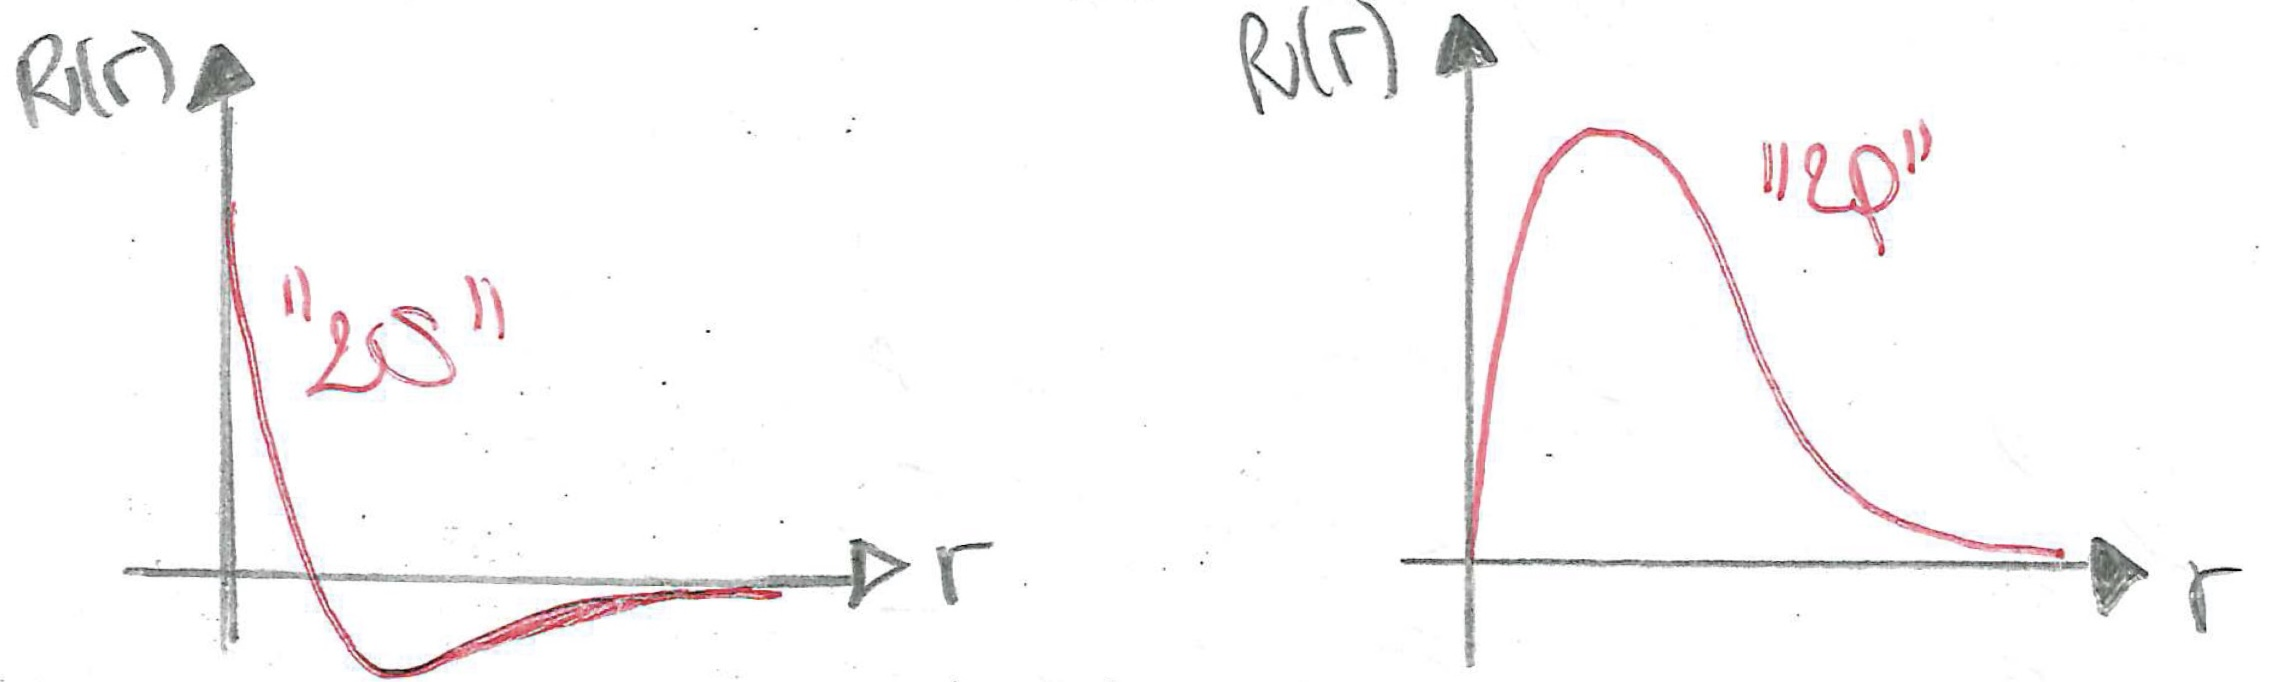
\includegraphics[]{images_ch5/hidrogen_levels.jpg}}
        Consideriamo a titolo di esempio l'atomo di idrogeno ed in particolare i livelli energetici $2s$ ($n=2$, $l=0$) e $2p$ ($n=2$, $l=1$). Nonostante $E_n$ dipenda solo dal numero quantico principale, e quindi i due livelli abbiano di fatto la stessa energia, le loro funzioni d'onda radiali differiscono.
    
        In particolare, l'orbitale con $l=0$ ha supporto\footnote{Nel senso che ha valore diverso da 0.} quando $r \rightarrow 0$ ed è quindi sensibile ad eventuali correzioni a corto raggio applicate al potenziale di Coulomb.
    
        Questo effetto, i.e. la differenza energetica tra i livelli \(^2S_{\nicefrac{1}{2}}\) e \(^2P_{\nicefrac{1}{2}}\), è stato misurato ed è detto \textit{Lamb Shift}.
    
        \marginnote{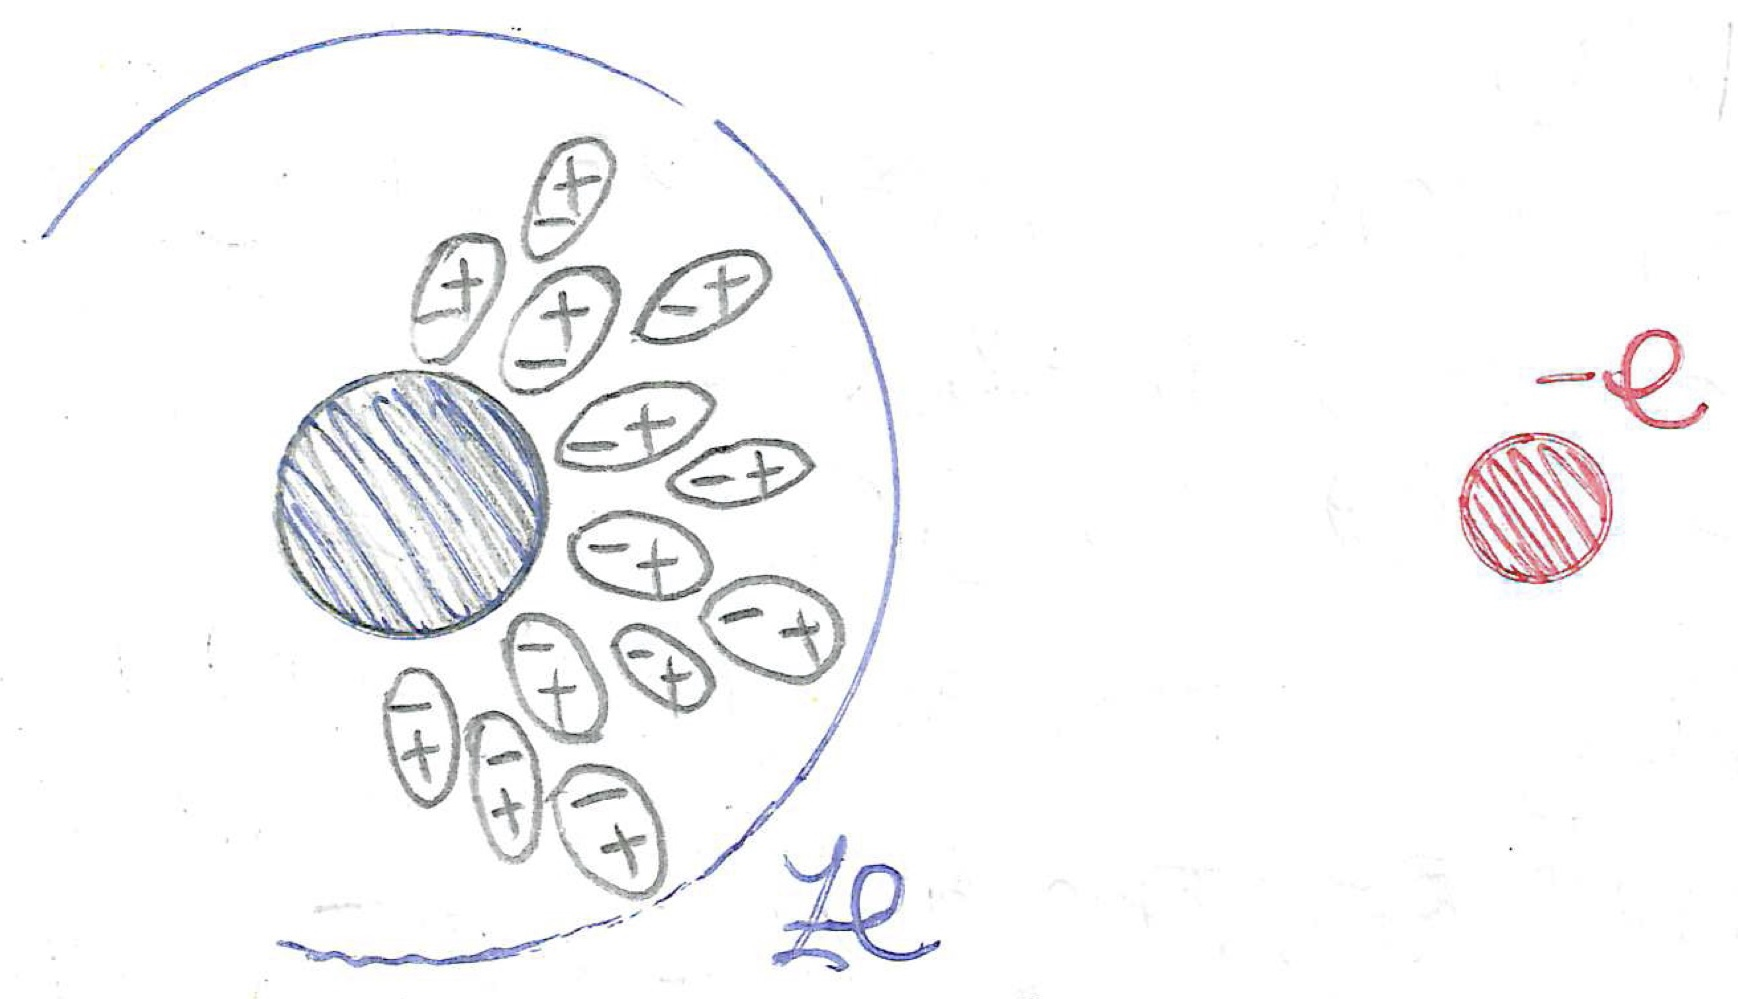
\includegraphics[]{images_ch5/electron_distant.jpg}}
        \item L'interpretazione fisica è la presenza di un \textit{effetto di polarizzazione del vuoto}. Infatti il termine di Uehling, quando l'elettrone si avvicina al nucleo, provoca una maggiore attrazione verso il nucleo stesso.
    
        In sostanza il vuoto risulta polarizzato e agisce come uno schermo per il potenziale, quando l'elettrone lontano dal nucleo.
    
        \marginnote{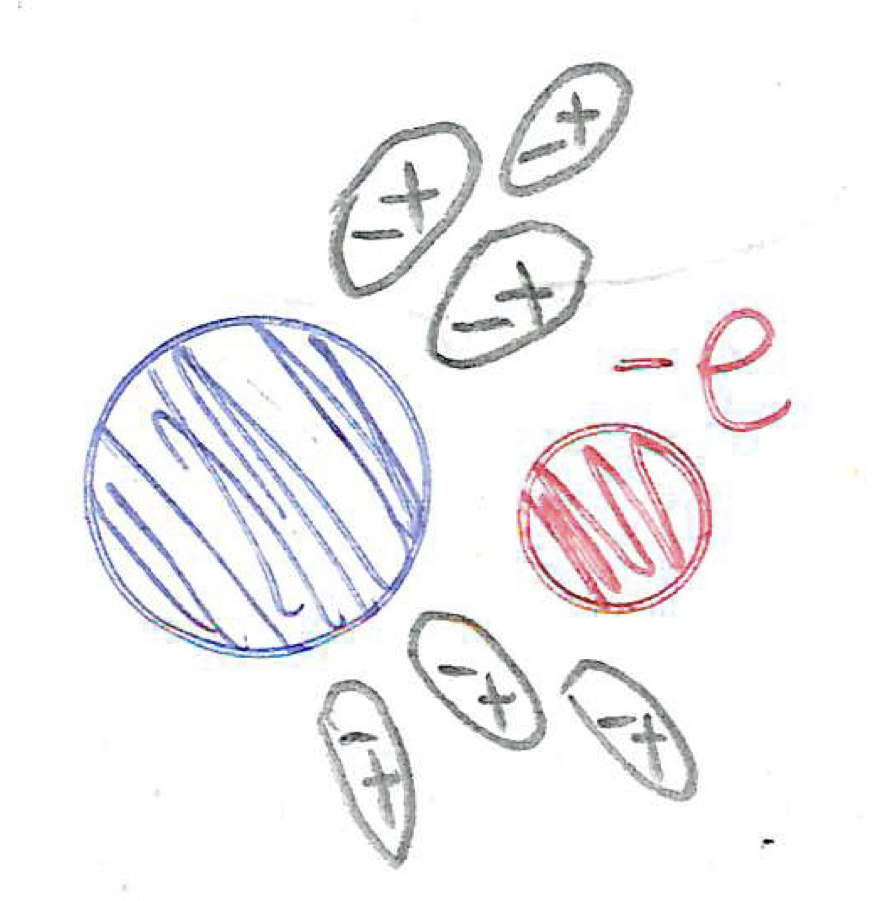
\includegraphics[]{images_ch5/electron_close.jpg}}
        Quando l'elettrone è sufficientemente vicino, invece, lo schermo viene penetrato e l'attrazione aumenta.
    \end{itemize}
    \label{note:uehlingterm_lambshift}
\end{nota}

\section{Il running della carica elettrica}
Consideriamo un processo in cui un fotone viene scambiato tra due correnti elettromagnetiche e studiamolo includendo la correzione ad un loop utilizzando la teoria rinormalizzata.
\[
\begin{tikzpicture}
    \begin{feynman}
        \diagram[horizontal'= d to b, inline=(a.base)] {
            i1 -- [fermion] a[dot, label=left:\(e_R\)] -- [fermion] i2,
            a --[photon, momentum=\(q\)] c[dot] --[fermion, half left] d[dot] --[photon] b[dot, label=right:\(e_R\)],
            d --[fermion, half left] c,
            f1 -- [fermion] b -- [fermion] f2
        };
        \draw [decoration={brace, mirror}, decorate, Gray] ([xshift=.0cm,yshift=-.5cm]a.south) -- ([xshift=.0cm,yshift=-.5cm]b.south) node [pos=.5, below] {\(\frac{(-ig_{\mu\nu})}{q^2 + i\varepsilon}\Big[ 1 + \overline{\Pi}_\text{1-loop}(q^2) \Big]\)};
    \end{feynman}
\end{tikzpicture}
\]
Indipendentemente dai dettagli riguardo le due correnti, sarà sempre presente la correzione agente sul propagatore del fotone che abbiamo visto nel paragrafo precedente, insieme alle due cariche fondamentali ai vertici.

Verrebbe allora da provare ad incorporare la correzione dell'auto-energia del fotone nella definizione di carica elettrica, definendola come “\textit{carica elettrica effettiva}:”

\begin{definition} \textbf{(Carica elettrica effettiva - 1 loop.)}
    \begin{equation}
        {
        \begin{aligned}
            &e_\text{eff}(q^2) = e_R\Big[ 1 + \overline{\Pi}_\text{1-loop}(q^2) \Big]^{\nicefrac{1}{2}} \\
            &\text{con } \overline{\Pi}_\text{1-loop}(0) = 0 \\
            & \text{ed } e_R=e_\text{phys} \text{ nello schema OS}
        \end{aligned}
        }
        \label{eq:effective_electric_charge}
    \end{equation}  
\end{definition}
La carica elettrica dipende quindi dalla scala di energia tipica del processo considerato.
In altre parole: la costante di accoppiamento non è costante, ma dipende dall'energia!

Prima abbiamo studiato il diagramma
\[
\feynmandiagram[horizontal'= d to b, inline=(a.base)] {
    i1 -- [anti fermion, edge label=\(p'\)] a[dot, label] -- [anti fermion, edge label=\(p\)] i2,
    a --[photon] c[dot] --[fermion, half left] d[dot] --[photon] b[large, crossed dot],
    d --[fermion, half left] c,
    };
\]
in cui la scala era determinata dal trasferimento di impulso, e abbiamo visto che \(\overline{\Pi}_\text{1-loop}(-|\Vec{q}|^2) \approx \frac{e_R^2}{60\pi^2} \frac{|\Vec{q}|^2}{m_R^2}\).

\subsection{Scattering \(e^-\mu^- \rightarrow e^-\mu^-\)}
\label{subsec:ee_mumu_scattering}
Consideriamo ora lo scattering \(e^-\mu^- \rightarrow e^-\mu^-\), che al tree-level si rappresenta:
\[
\feynmandiagram[vertical= a to b]{
    i1[particle=$e^-(p_1)$] --[fermion] a --[fermion] i2[particle=$e^-(p_3)$],
    a --[photon, momentum=$q$] b,
    f1[particle=$\mu^-(p_4)$] --[anti fermion] b --[anti fermion] f2[particle=$\mu^-(p_2)$]}; 
\]
con \(p_1 = q + p_3\) , \(p_2 + q = p_4\) .
\begin{nota}
    Sviluppando la cinematica nel centro di massa, si arriva senza troppe difficoltà alle seguenti relazioni:
    \marginnote{dove utilizziamo la funzione triangolo \(\lambda(a,b,c) = a^2 + b^2 + c^2 - 2ab - 2ac - 2cb\) }
    \begin{align*}
        &p_1 = (E_e, 0,0,|\Vec{p}|)  &p_3 = (E_e, |\Vec{p}|\sin\vartheta , 0, |\Vec{p}|\cos\vartheta) \\
        &p_2 = (E_\mu, 0,0,-|\Vec{p}|)  &p_4 = (E_\mu, -|\Vec{p}|\sin\vartheta , 0, -|\Vec{p}|\cos\vartheta)  \\
        &E_e = \frac{\sqrt{s}}{2}\bigg( 1 + \frac{m_e^2 - m_\mu^2}{s} \bigg)  &E_\mu = \frac{\sqrt{s}}{2}\bigg( 1 + \frac{m_\mu^2 - m_e^2}{s} \bigg) \\
        &|\Vec{p}|^2 = \frac{1}{4s}\lambda(s, m_e^2, m_\mu^2)&
    \end{align*}
    Essendo per costruzione \(q=p_1 - p_3\), sostituendo e svolgendo pochi conti si arriva a trovare: \marginnote{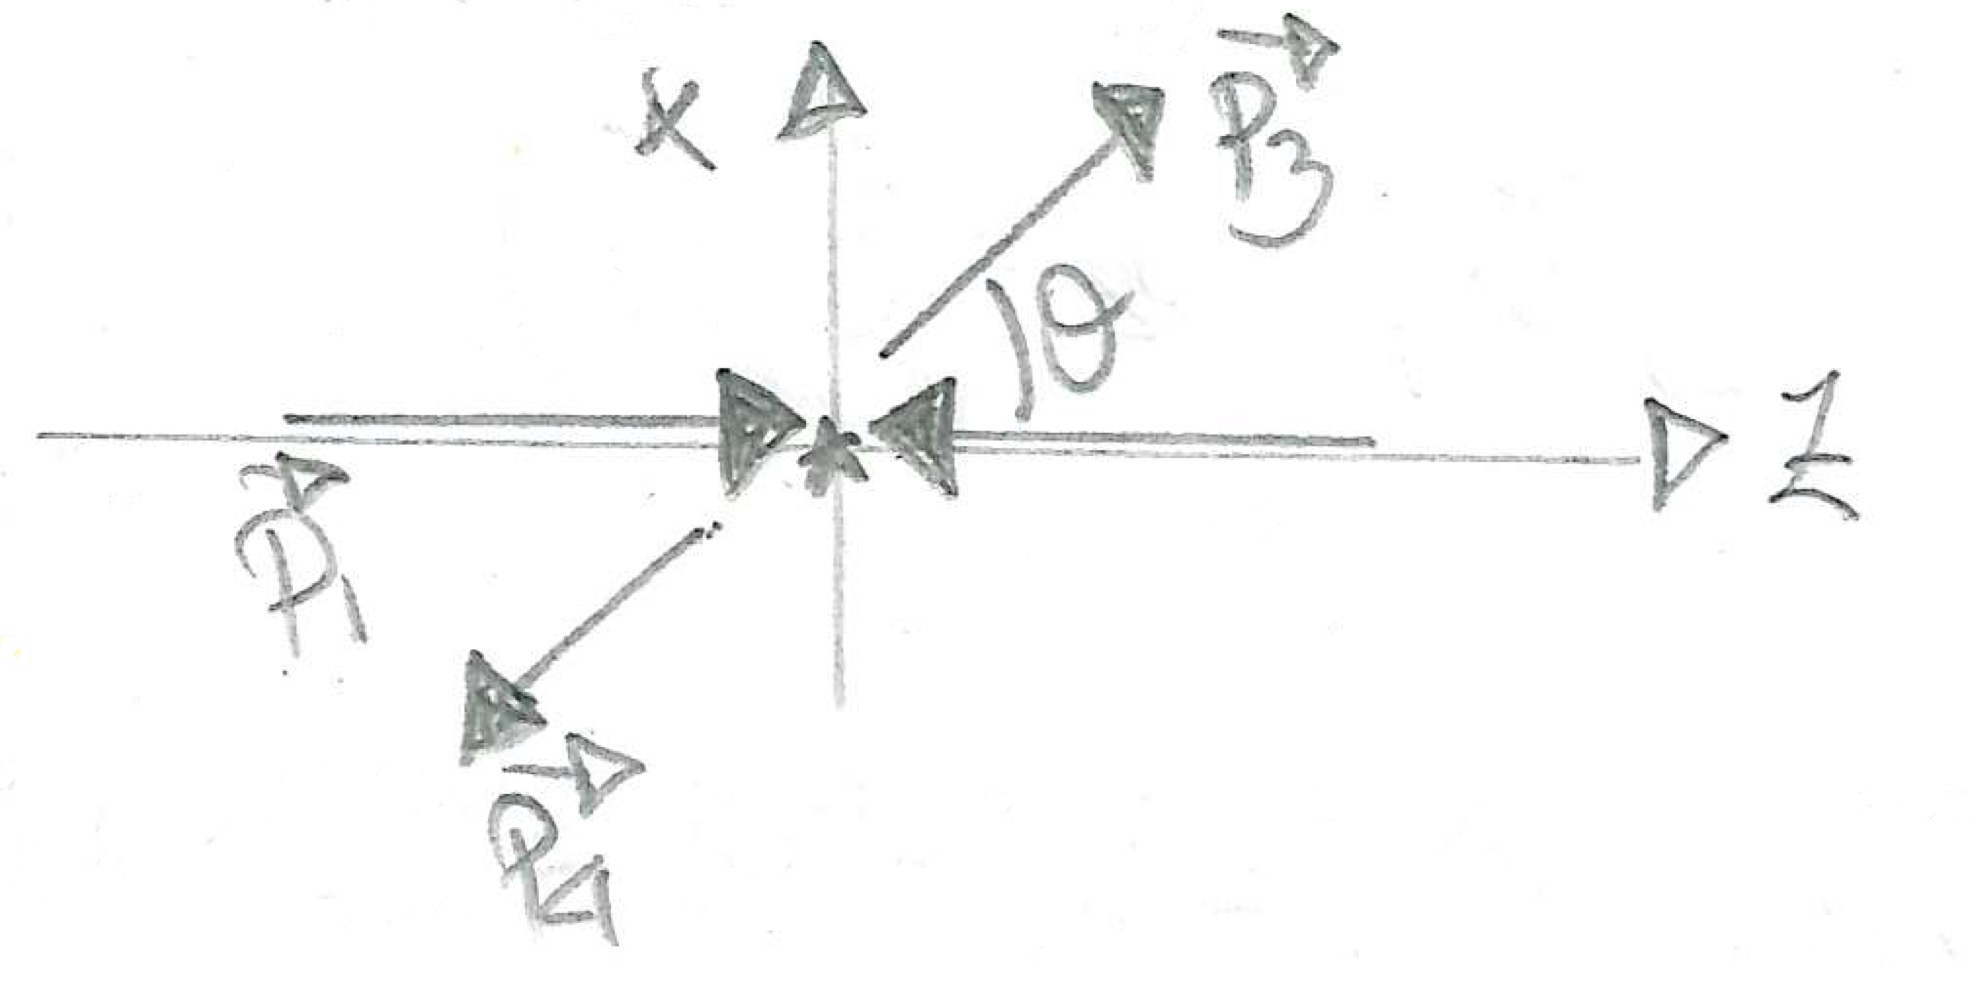
\includegraphics[]{images_ch5/ee_mumu_com.jpg}}
    \[
    \boxed{q^2 = - |\Vec{q}|^2 = -2|\Vec{p}|^2\big(1-\cos\vartheta\big)}
    \]
    Ma \(2|\Vec{p}|^2\big(1-\cos\vartheta\big) > 0\) sempre, quindi il quadrato del 4-impulso trasferito è sempre negativo. $q$ è un quadrivettore di tipo spazio.
    \label{note:COM_ee_mumu_tchannel}
\end{nota}

Ragioniamo ora come prima, con l'obiettivo di introdurre anche in questo caso una carica elettrica effettiva.

In questo caso, al contrario dello scattering Coulombiano, assumiamo di essere in regime ultra-relativistico, i.e. \(|\Vec q|^2\gg m_e^2,m_\mu^2\).

Un importante aspetto di cui va tenuto conto è il fatto che, considerando il loop che fornisce la carica effettiva, possiamo avere sia un elettrone che un muone. Questo si riflette in una somma di due diagrammi, invece di uno, più il controtermine.
\[
\feynmandiagram[vertical= a to b, inline=(c.base)] {
    i1[particle=$e^-$] --  a[dot] --  i2[particle=$e^-$],
    a --[photon] c[dot] --[fermion, half left, edge label=\(e^-\)] d[dot] --[photon] b[dot],
    d --[fermion, half left] c,
    f1[particle=$\mu^-$] --  b --  f2[particle=$\mu^-$]
};
+
\feynmandiagram[vertical= a to b, inline=(c.base)] {
    i1[particle=$e^-$] --  a[dot] --  i2[particle=$e^-$],
    a --[photon] c[dot] --[fermion, half left, edge label=\(\mu^-\)] d[dot] --[photon] b[dot],
    d --[fermion, half left] c,
    f1[particle=$\mu^-$] --  b --  f2[particle=$\mu^-$]
};
+
\feynmandiagram[vertical= a to b, inline=(c.base)] {
    i1[particle=$e^-$] --  a[dot] --   i2[particle=$e^-$],
    a --[photon] d[small, crossed dot] --[photon] b[dot],
    f1[particle=$\mu^-$] --   b --   f2[particle=$\mu^-$]
};
\]

Segue quindi che, in questo caso:
\[
\overline\Pi_\text{1-loop} = \frac{8e_R^2}{16\pi^2} \int\limits_0^1 dx \, x(1-x) 
\Bigg\{
\log\bigg[ \frac{m_e^2 - x(1-x)q^2}{m_e^2} \bigg] + \log\bigg[ \frac{m_\mu^2 - x(1-x)q^2}{m_\mu^2} \bigg]
\Bigg\}
\]
dove \(m_{e,\mu}\) sono le masse rinormalizzate per l'elettrone ed il muone.

Ora, ricordando l'approssimazione ultra-relativistica, possiamo dire che per $m_R$ generica 
\[
\log\bigg[ \frac{m_R^2 - x(1-x)q^2}{m_R^2} \bigg] \approx \log\bigg[ \frac{- x(1-x)q^2}{m_R^2}\bigg] = \log\bigg(\frac{- q^2}{m_R^2}\bigg) + \log x(1-x)
\]

Siccome $\log x(1-x)$, una volta integrato, porta un contributo costante (ed anche piuttosto piccolo), possiamo trascurarlo. Il che significa che: 

\[
\boxed{
\int\limits_0^1 dx \, x(1-x) \log\bigg[ \frac{m_R^2 - x(1-x)q^2}{m_R^2} \bigg] \approx
\frac{1}{6}\log\bigg(\frac{- q^2}{m_R^2}\bigg) }
\]

Perciò, sulla base della sua definizione (\ref{eq:effective_electric_charge}), la carica effettiva (al quadrato in questo caso) sarà:

\begin{equation}
    \boxed{
    e_\text{eff}^2 = e_R^2\bigg[ 1 + \frac{e_R^2}{12\pi^2}\log\bigg(\frac{- q^2}{m_e^2}\bigg) +  \frac{e_R^2}{12\pi^2}\log\bigg(\frac{- q^2}{m_\mu^2}\bigg)\bigg]}
    \label{eq:ee_mumu_runningcoupling}
\end{equation}
con \(-q^2 = |\Vec{q}|^2 \gg m_e^2, m_\mu^2 \).

Troviamo quindi che la forza dell'interazione cresce ad alte energie (ovvero a piccole distanze).
Il coupling, infatti, cresce in maniera logaritmica con l'aumentare della scala di energia alla quale viene svolto l'esperimento, i.e. il valore tipico di $q^2$.

Questo effetto è noto come \textbf{running coupling}.

\subsection{Generalità del running coupling}

Abbiamo derivato questo risultato considerando esplicitamente lo scambio di impulso tramite t-channel, ma il risultato è più generale:

Ogni ampiezza che coinvolge un trasferimento di energia (o impulso) $Q\gg m_e$ in QED è caratterizzata da un coupling effettivo dipendente da tale trasferimento di energia \(e_\text{eff}(Q)\) che ad un loop si scrive:
\begin{equation}
    e_\text{eff}^2(Q^2) = e_R^2\bigg[ 1 + 
    \underbrace{\frac{e_R^2}{12\pi^2}\log\bigg(\frac{Q^2}{m_R^2}\bigg)}_{\substack{\text{correzione dovuta}\\\text{al solo loop}\\\text{con l'elettrone}}}
    \bigg]
    \label{eq:general_runningcoupling_1loop}
\end{equation}

\subsubsection{Commenti}
\begin{enumerate}
    \item[\textbf{1)}] L'equazione (\ref{eq:general_runningcoupling_1loop}) si applica alla QED più semplice possibile, composta solo da fotoni ed elettroni e da nessun altro campo. Nella realtà il fotone si accoppia anche con i quark, i muoni o i tau. Limitando la trattazione ad un loop, l'apporto di queste particelle al running del coupling è simile a quello dell'elettrone, eccetto per la massa e la carica.

     \item[\textbf{2)}] Volendo possiamo spingerci oltre con il calcolo inserendo nel propagatore ordini superiori ad un loop. Ci riferiremo a tale propagatore come “propagatore resummato”\footnote{dall'inglese \textit{resummed}, in pratica è come se fosse il propagatore vestito}.

     Con riferimento all'equazione (\ref{eq:dressed_photon_propagator_summary}), è chiaro che il fattore che vogliamo introdurre nella definizione di carica efficace è il residuo $\sqrt Z_3$, implementando la notazione di rinormalizzazione per mezzo dei contro-termini al denominatore. Scriviamo quindi:

    \begin{equation}
        e_\text{eff}^2(Q^2) = \frac{e_R^2}{1 - \overline\Pi(Q^2)} 
        \xrightarrow[]{Q^2\gg m_R^2}
        \frac{e_R^2}{ 1 - \frac{e_R^2}{12\pi^2}\log\bigg(\frac{Q^2}{m_R^2}\bigg)}
        \label{eq:general_runningcoupling_resummed}
    \end{equation}

    Ci accorgiamo immediatamente della presenza di una singolarità nel punto noto come \textbf{polo di Landau}:
    \begin{equation}
        Q_\star^2 = m_R\exp{\frac{12\pi^2}{e_R^2}}
        \label{eq:Landau_pole}
    \end{equation}

    \item[\textbf{3)}] Abbiamo introdotto il propagatore vestito fotonico, definito diagrammaticamente come in sezione \ref{subsec:dressed_photon_propagator}:
    \begin{align*}
        \begin{tikzpicture}[baseline=\plusheight]
          \begin{feynman}[small] % dressed electron propagator diagram
          \vertex[dot] (a) at (-1.3,0) {} ;
          \vertex[large, blob] (m) at (0,0) {};
          \vertex[dot] (b) at (1.3,0) {};
          \diagram*[] {
            (a)--[photon, momentum={$q$}] (m) --[photon] (b)};
          \end{feynman}
      \end{tikzpicture} 
      =
      \begin{tikzpicture}[baseline=\plusheight]
          \begin{feynman}[every blob={/tikz/fill=white!100}]
              \vertex[blob] (m) at (0,0) {1PI};
              \vertex[small,dot] (a) at (-1,0) {} ;
              \vertex[small,dot] (b) at (1,0) {};
              \diagram*[] {
                (a)-- [photon](m) --[photon] (b)
                };
          \end{feynman}
      \end{tikzpicture} 
      +
      \begin{tikzpicture}[baseline=\plusheight]
          \begin{feynman}[ every blob={/tikz/fill=white!100}]
              \vertex[small,dot] (a) at (-1,0) {} ;
              \vertex[blob] (m) at (0,0) {1PI};
              \vertex[blob] (m1) at (1,0) {1PI};
              \vertex[small,dot] (c) at (2,0) {};
              \diagram*[] {
                (a)-- [photon](m) --[photon] (m1) --[photon] (c)
                };
          \end{feynman}
      \end{tikzpicture} 
      + \cdot\cdot\cdot
    \end{align*}
    fermandoci alla trattazione ad 1 loop per quanto riguarda i diagrammi 1PI. Questa procedura è consistente dal punto di vista perturbativo? Per capirlo utilizziamo i seguenti argomenti:
    \begin{itemize}
        \item Stiamo includendo, nella somma sopra, diagrammi a due loop di ordine \(\mathscr{O}(e_R^4)\) nell'espansione perturbativa.
        \begin{align*}
            \begin{tikzpicture}[baseline=\plusheight]
              \begin{feynman}[small] % dressed electron propagator diagram
                  \vertex[dot] (a) at (-1.3,0) {} ;
                  \vertex[large, blob] (m) at (0,0) {};
                  \vertex[dot] (b) at (1.3,0) {};
                  \diagram*[small] {
                    (a)--[photon] (m) --[photon] (b)};
              \end{feynman}
            \end{tikzpicture} 
            \supset 
            \begin{tikzpicture}[baseline=\plusheight]
                \begin{feynman}[every blob={/tikz/fill=white!100}]
                    \diagram[small, horizontal= a to b, layered layout] {
                        a[dot] --[photon] c[dot] --[fermion, half left] d[dot] --[photon] b[dot],
                        d --[fermion, half left] c,
                        b --[fermion, half left] f[dot] --[photon] g[dot],
                        f --[fermion, half left] b,
                    };
                \end{feynman}
            \end{tikzpicture} 
            \propto e_R^4
        \end{align*}
        
        \item Non abbiamo invece incluso diagrammi del tipo seguente

        \begin{align*}
            \begin{tikzpicture}[baseline=\plusheight]
              \begin{feynman}[small] % dressed electron propagator diagram
                  \vertex[dot] (a) at (-1.3,0) {} ;
                  \vertex[large, blob] (m) at (0,0) {};
                  \vertex[dot] (b) at (1.3,0) {};
                  \diagram*[] {
                    (a)--[photon] (m) --[photon] (b)};
              \end{feynman}
            \end{tikzpicture} 
            \not\supset 
            \begin{tikzpicture}[baseline=\plusheight]
                \begin{feynman}[small]
                    \vertex[dot] (a) at (-1,0) {} ;
                    \vertex[dot] (v1) at (0,0) {};
                    \vertex[dot] (vup) at (0.5,0.5) {};
                    \vertex[dot] (v2) at (1,0) {};
                    \vertex[dot] (vdown) at (0.5,-0.5) {};
                    \vertex[dot] (c) at (2,0) {};
                    \diagram*[] {
                        (a)-- [photon](v1) --[quarter left] (vup) --[quarter left] (v2) --[photon] (c),
                        (v1) --[quarter right] (vdown) --[quarter right] (v2),
                        (vup) --[photon] (vdown)
                    }; 
                \end{feynman}
            \end{tikzpicture} 
            +
            \begin{tikzpicture}[baseline=\plusheight]
                \begin{feynman}[small]
                    \vertex[dot] (a) at (-1,0) {} ;
                    \vertex[dot] (v1) at (0,0) {};
                    \vertex[dot] (vup) at (0.05,0.25) {};
                    \vertex[dot] (v2) at (1,0) {};
                    \vertex[dot] (vdown) at (0.95,0.25) {};
                    \vertex[dot] (c) at (2,0) {};
                    \diagram*[] {
                        (a)-- [photon](v1) --[half left] (v2) --[photon] (c),
                        (v1) --[half right] (v2),
                        (vup) --[photon, half right, looseness=0.3] (vdown)
                    }; 
                \end{feynman}
            \end{tikzpicture}
            \propto e_R^4
        \end{align*}
        anch'essi di ordine \(\mathscr{O}(e_R^4)\)
    \end{itemize}
    La logica con cui lo facciamo è la seguente:
    \begin{itemize}
        \item[-] Diagrammi ad \textbf{un loop} producono termini \(\sim e_R^2\log{Q^2} \approx \alpha \log{Q^2}\), lo abbiamo visto esplicitamente.
        \item[-] Di conseguenza diagrammi a \textbf{due loop} produrranno termini \(\sim\alpha^2 \log^2{Q^2}\), come fossero il quadrato dei diagrammi ad un loop.
        \item[-] Al contrario, diagrammi come quelli che non stiamo considerando, daranno correzioni \(\sim\alpha^2\log{Q^2}\), che sono di ordine $\alpha^2$, ma hanno solo un logaritmo. Questi termini sono detti \textit{sotto-dominanti}\footnote{Dall'inglese \textit{subleading}, in pratica sono trascurabili rispetto al contributo dei termini dominanti.} nel limite di alto $Q^2$.
    \end{itemize}

    In conclusione, diciamo che la serie considerata fornisce una \textbf{resummazione}\footnote{dall'inglese \textit{resummation}, è una procedura utilizzata per fornire un'approssimazione più precisa possibile sfruttando calcoli ad ordini sempre maggiori combinati in un'unica somma.} dei cosiddetti logaritmi dominanti \(\alpha^n\log^n Q^2\)
\end{enumerate}

\section{L'equazione del Gruppo di Rinormalizzazione}
Partiamo dall'equazione (\ref{eq:general_runningcoupling_resummed}) ed invertiamola, moltiplichiamo e dividiamo per \(\mu^2\) nel logaritmo e separiamolo, ottenendo la seguente espressione:
\[
\frac{1}{e_\text{eff}^2(Q^2)} = 
\underbrace{\frac{1}{e_R^2} - \frac{1}{12\pi^2}\log{\frac{\mu^2}{m_R^2}}}_{=\nicefrac{1}{e_\text{eff}^2(\mu^2)}}
- \frac{1}{12\pi^2}\log{\frac{Q^2}{\mu^2}}
\]
Se ora deriviamo in $d\mu$, otteniamo:
\[
0 = \frac{(-2)}{e_\text{eff}^3(\mu^2)} \frac{de_\text{eff}(\mu^2)}{d\mu} - \frac{1}{12\pi^2}\cdot\frac{\Ccancel[Green]{\mu^2}}{\Ccancel[Red]{Q^2}}\cdot \frac{(-2)\Ccancel[Red]{Q^2}}{\mu^{\Ccancel[Green]{3}}} 
\]
In definitiva, possiamo scrivere quella che viene definita come equazione del gruppo di rinormalizzazione (\textbf{RGE}) per il coupling elettrico ad un loop:
\begin{equation}
    \boxed{\mu\frac{de_\text{eff}}{d\mu} = \frac{e_\text{eff}^3}{12\pi^2} }
    \label{eq:RGE_electr_1loop}
\end{equation}

La RGE è un'equazione differenziale a variabili separabili che controlla il running del coupling effettivo. Inoltre il RHS è noto come funzione beta per la QED ad un loop\footnote{Quando diciamo “ad un loop”, intendiamo che nei diagrammi 1PI stiamo tenendo conto al massimo dei diagrammi con 1 loop. Aumentando i loop considerati, si aggiungono termini alla funzione beta.}, ma su questo torneremo in seguito, nella sezione \ref{subsec:alternative_rgf}.

Il variare di \(e_\text{eff}(\mu)\) al variare di \(\mu\) è detto \textit{flusso del gruppo di rinormalizzazione} (\textbf{RGF}).

\begin{nota}
    \textbf{Check di consistenza.} \\
    Integriamo la (\ref{eq:RGE_electr_1loop}) e verifichiamo che effettivamente si ritrova la (\ref{eq:general_runningcoupling_resummed}). In particolare, dato che \(d(\mu^2) = 2\mu d\mu\), sostituiamo \(d\mu = \frac{1}{2\mu}d\mu^2\) e integriamo nel seguente modo separando le variabili:
    
    \[
    \int \limits_{e_\text{eff}(m^2)=e_R}^{e_\text{eff}(Q^2)} \frac{de_\text{eff}}{e_\text{eff}^3} = \frac{1}{24\pi^2} \int\limits_{\mu_{\text{ref}}^2=m^2}^{\mu^2=Q^2}\frac{d\mu^2}{\mu^2}
    \]
    
    Notiamo come nell'approssimazione in cui stiamo lavorando, il limite di bassa energia che definisce il valore osservato della carica elettrica (e rappresenta una condizione al contorno necessaria per risolvere l'equazione) è \(\mu_{\text{ref}}^2 = m^2\) e non \(\mu_{\text{ref}}^2 = 0\).
    
    Procedendo con l'integrazione otteniamo:
    \[
    -\frac{1}{2}\bigg[ \frac{1}{e_\text{eff}^2(Q^2)} - \frac{1}{e_R^2(Q^2)} \bigg] = \frac{1}{24\pi^2} \big( \log Q^2 - \log m^2 \big)
    \]
    E da qui non è difficile ricavare l'equazione di partenza:
    \[
    \frac{1}{e_\text{eff}^2(Q^2)} = 
    \frac{1}{e_R^2} - \frac{1}{12\pi^2}\log{\frac{Q^2}{m^2}}
    \] \qed
    
\end{nota}

\subsection{RGF alternativi}
\label{subsec:alternative_rgf}

Quanto discusso nel caso della QED è valido per una generica QFT: le costanti di accoppiamento $\lambda(\mu)$ dipendono dall'energia ed il loro “running” è descritto dalla corrispondente RGE, la cui struttura schematica, comprensiva di condizione al contorno, è:
\begin{equation}
    \mu\frac{d\lambda(\mu)}{d\mu} = \beta(\lambda) ~~,~~ \lambda(\mu_\text{ref})=\lambda_0
    \label{eq:RGE_generic}
\end{equation}
La funzione beta è specifica per il singolo coupling. Per esempio, in QED, \(\lambda = e\) e \(\beta(\lambda) = \frac{e^3}{12\pi^2}\).

Dipendentemente dal segno della funzione beta, si hanno 3 comportamenti differenti per il flusso del gruppo di rinormalizzazione:
\begin{enumerate}
    \item[\textbf{1)}] Se \(\underline{\beta(\lambda) > 0}\), \(\lambda(\mu)\) incrementa \textcolor{Gray}{(decrementa)} con l'aumentare \textcolor{Gray}{(decrementare)} di $\mu$.

    Questo è il caso della QED. Quando \(\lambda(\mu)\approx 4\pi\) la teoria diventa non perturbativa.
    
    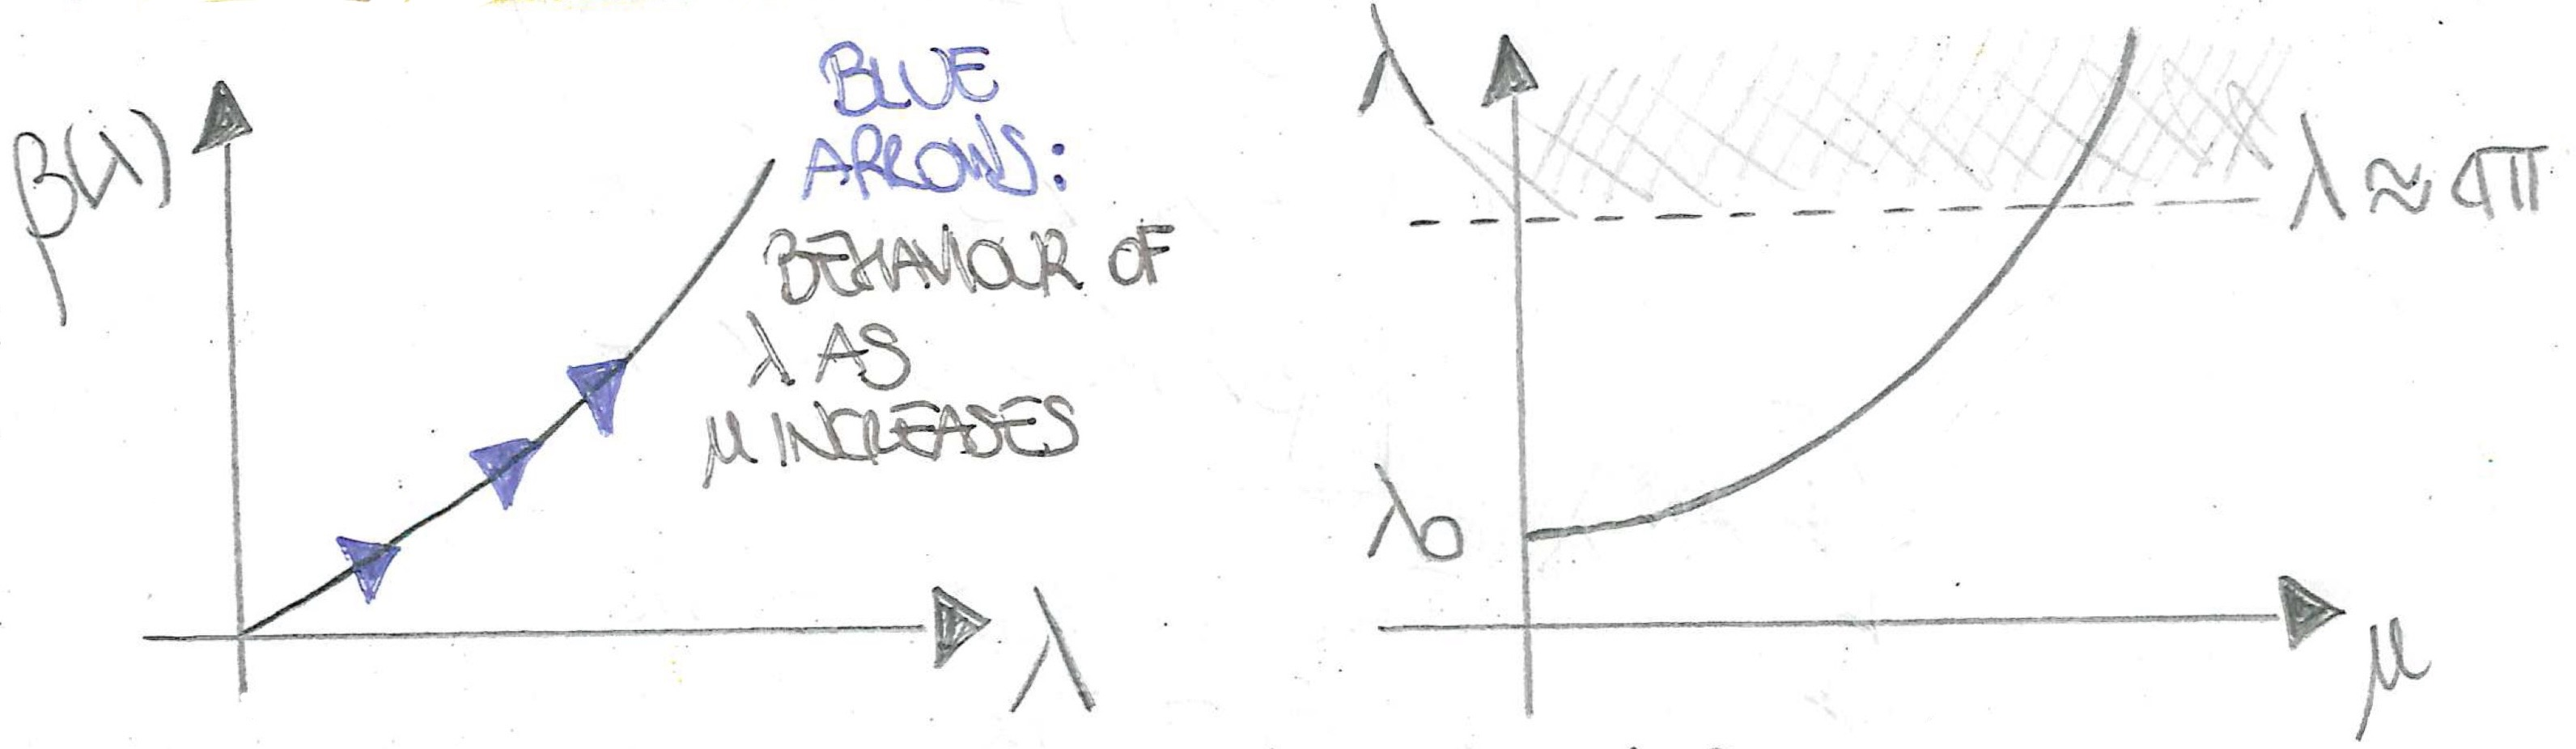
\includegraphics[]{images_ch5/beta_case1.jpg}
    
    \item[\textbf{2)}] Se \(\underline{\beta(\lambda) < 0}\), \(\lambda(\mu)\) decrementa \textcolor{Gray}{(incrementa)} con l'aumentare \textcolor{Gray}{(decrementare)} di $\mu$.


    Questo caso è detto di “libertà asintotica”: la teoria diventa non perturbativa nel regime delle alte energie. Un esempio può essere la QCD.
    
    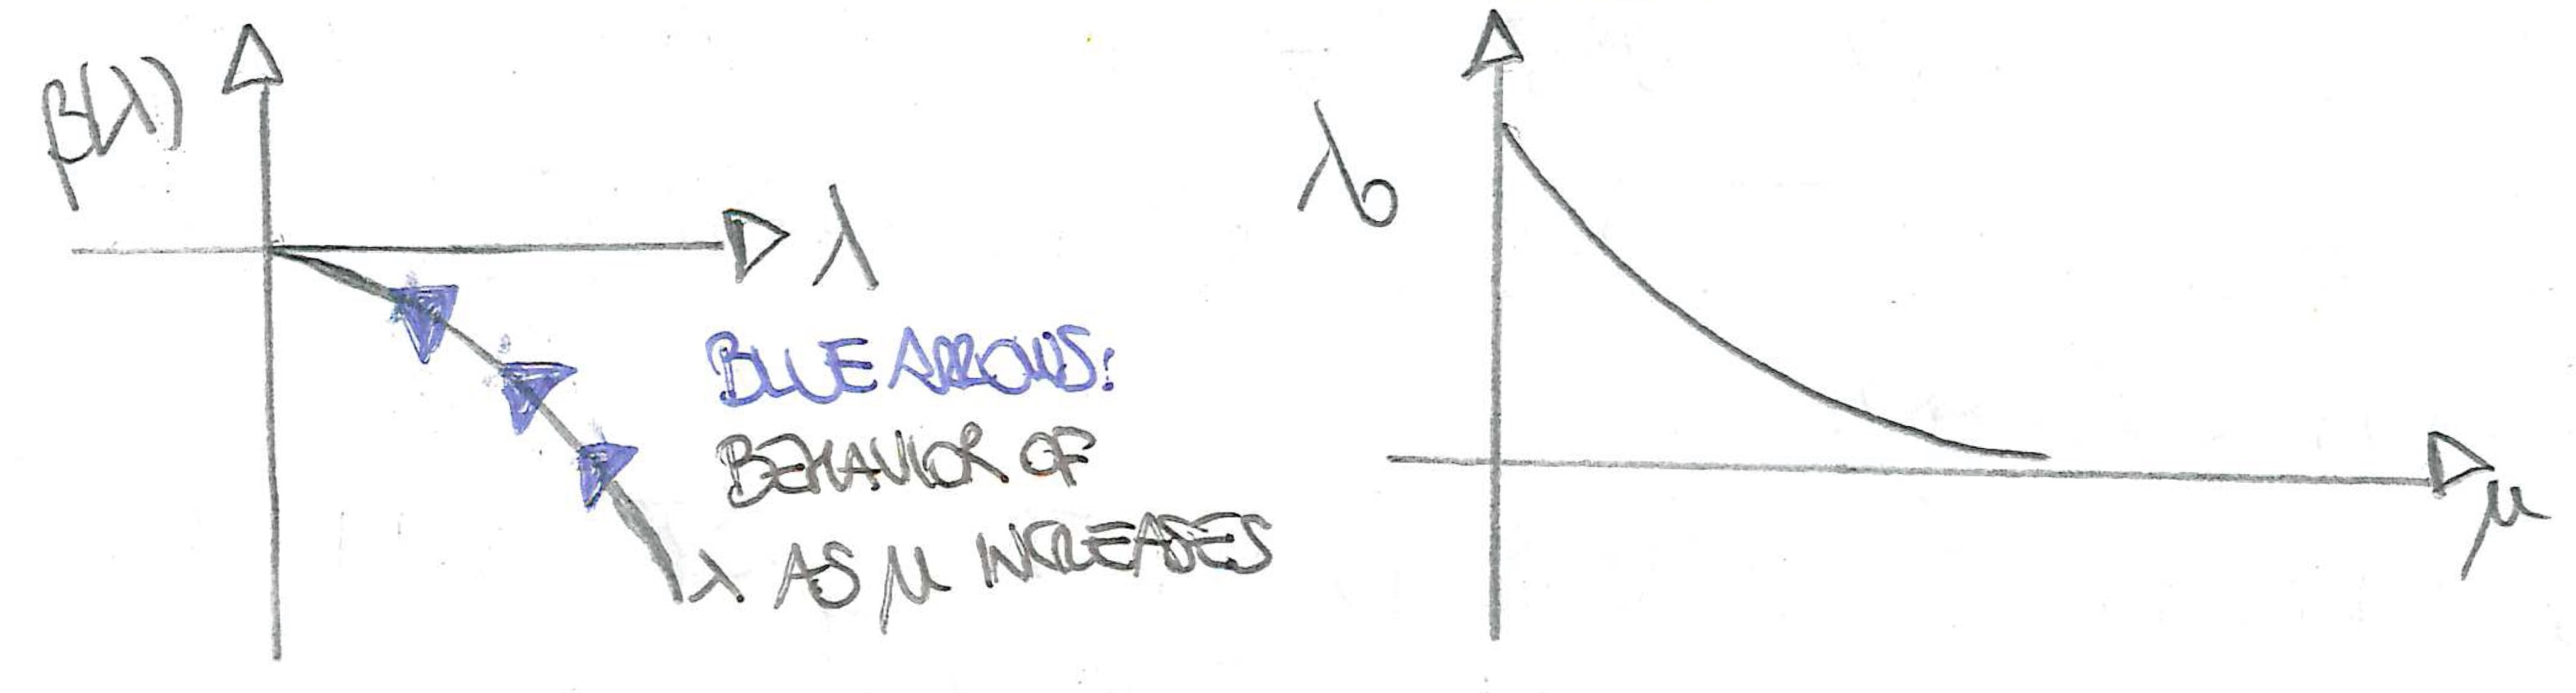
\includegraphics[]{images_ch5/beta_case2.jpg}
    
    \item[\textbf{3)}] Se \(\underline{\beta(\lambda) = 0}\), \(\lambda(\mu)\) non dipende da $\mu$.

    In questo caso la teoria è detta “scale-independent” o conforme.
\end{enumerate}

Tuttavia quelli appena elencati sono casi estremi, può accadere che $\beta(\lambda)$ sia una mistura dei tre, ad esempio:

\begin{itemize}
    \item \textbf{Punto fisso ultravioletto non banale}\marginnote{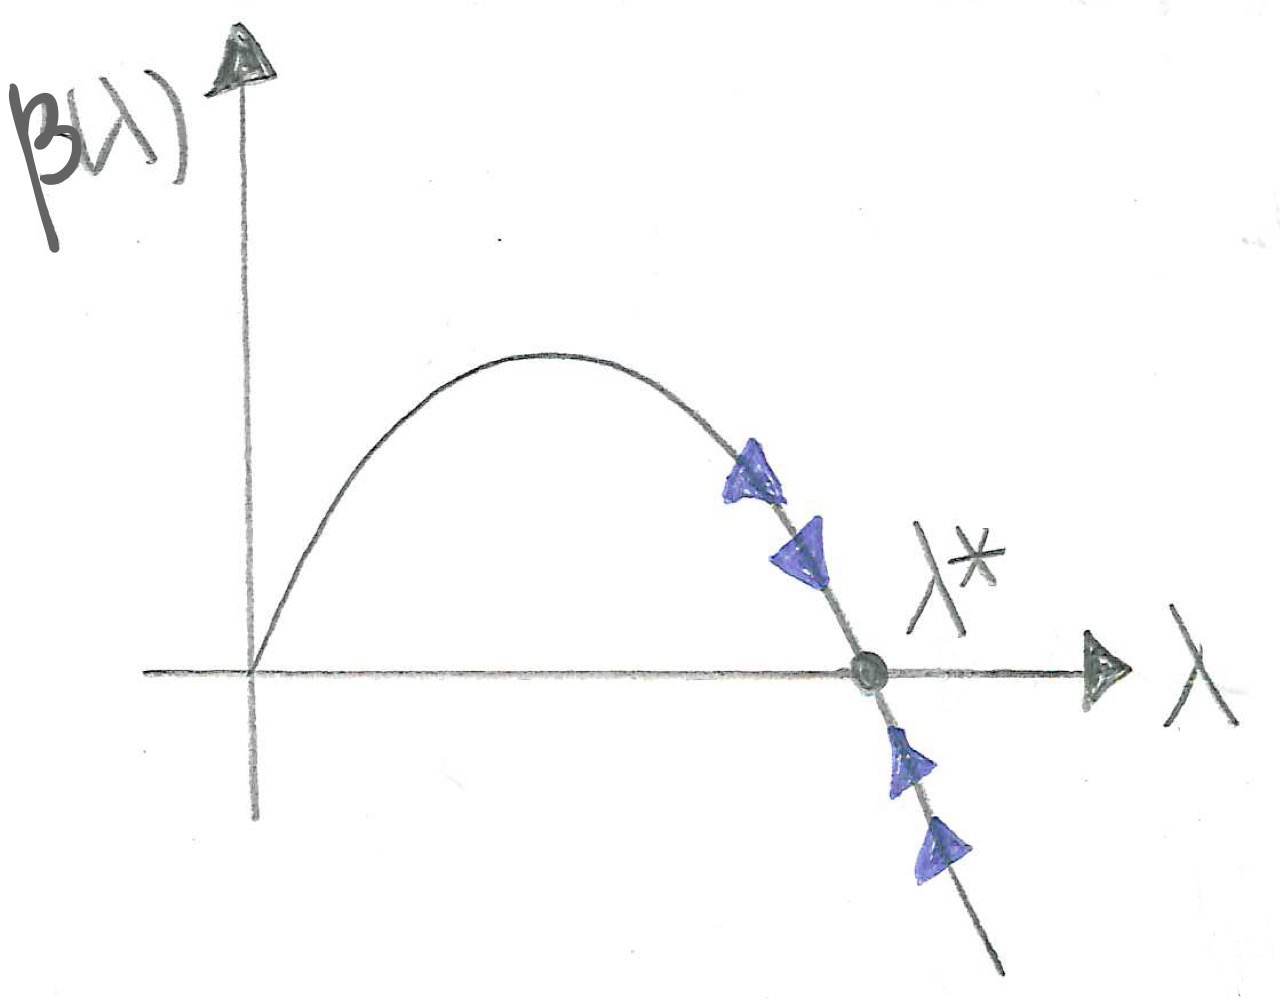
\includegraphics[]{images_ch5/uv_fixed.jpg} \\ Plot schematico di una funzione beta con punto fisso ultravioletto. Le frecce blu indicano l'andamento di \(\lambda\) con l'aumentare di $\mu$.}
    Consideriamo il caso seguente, rappresentato schematicamente a lato:
    \begin{align*}
        &\beta(\lambda^\ast) = 0 ~~,~~ \beta'(\lambda^\ast)<0 \\
        &\beta(\lambda) > 0 ~~,~~ \lambda < \lambda^\ast \\
        &\beta(\lambda) < 0 ~~,~~ \lambda > \lambda^\ast
    \end{align*}
    Questo accade se abbiamo \(\beta(\lambda) > 0\) all'ordine inferiore in $\lambda$ ma poi, per via di termine di ordine superiore che assumono rilevanza con l'aumentare di $\lambda$, \(\beta(\lambda)\) decresce e cambia di segno.

    $\lambda^\ast$ è detto punto fisso ultravioletto, in quanto $\lambda$ è sempre attratto da $\lambda^\ast$ ad alta energia $\mu$.

    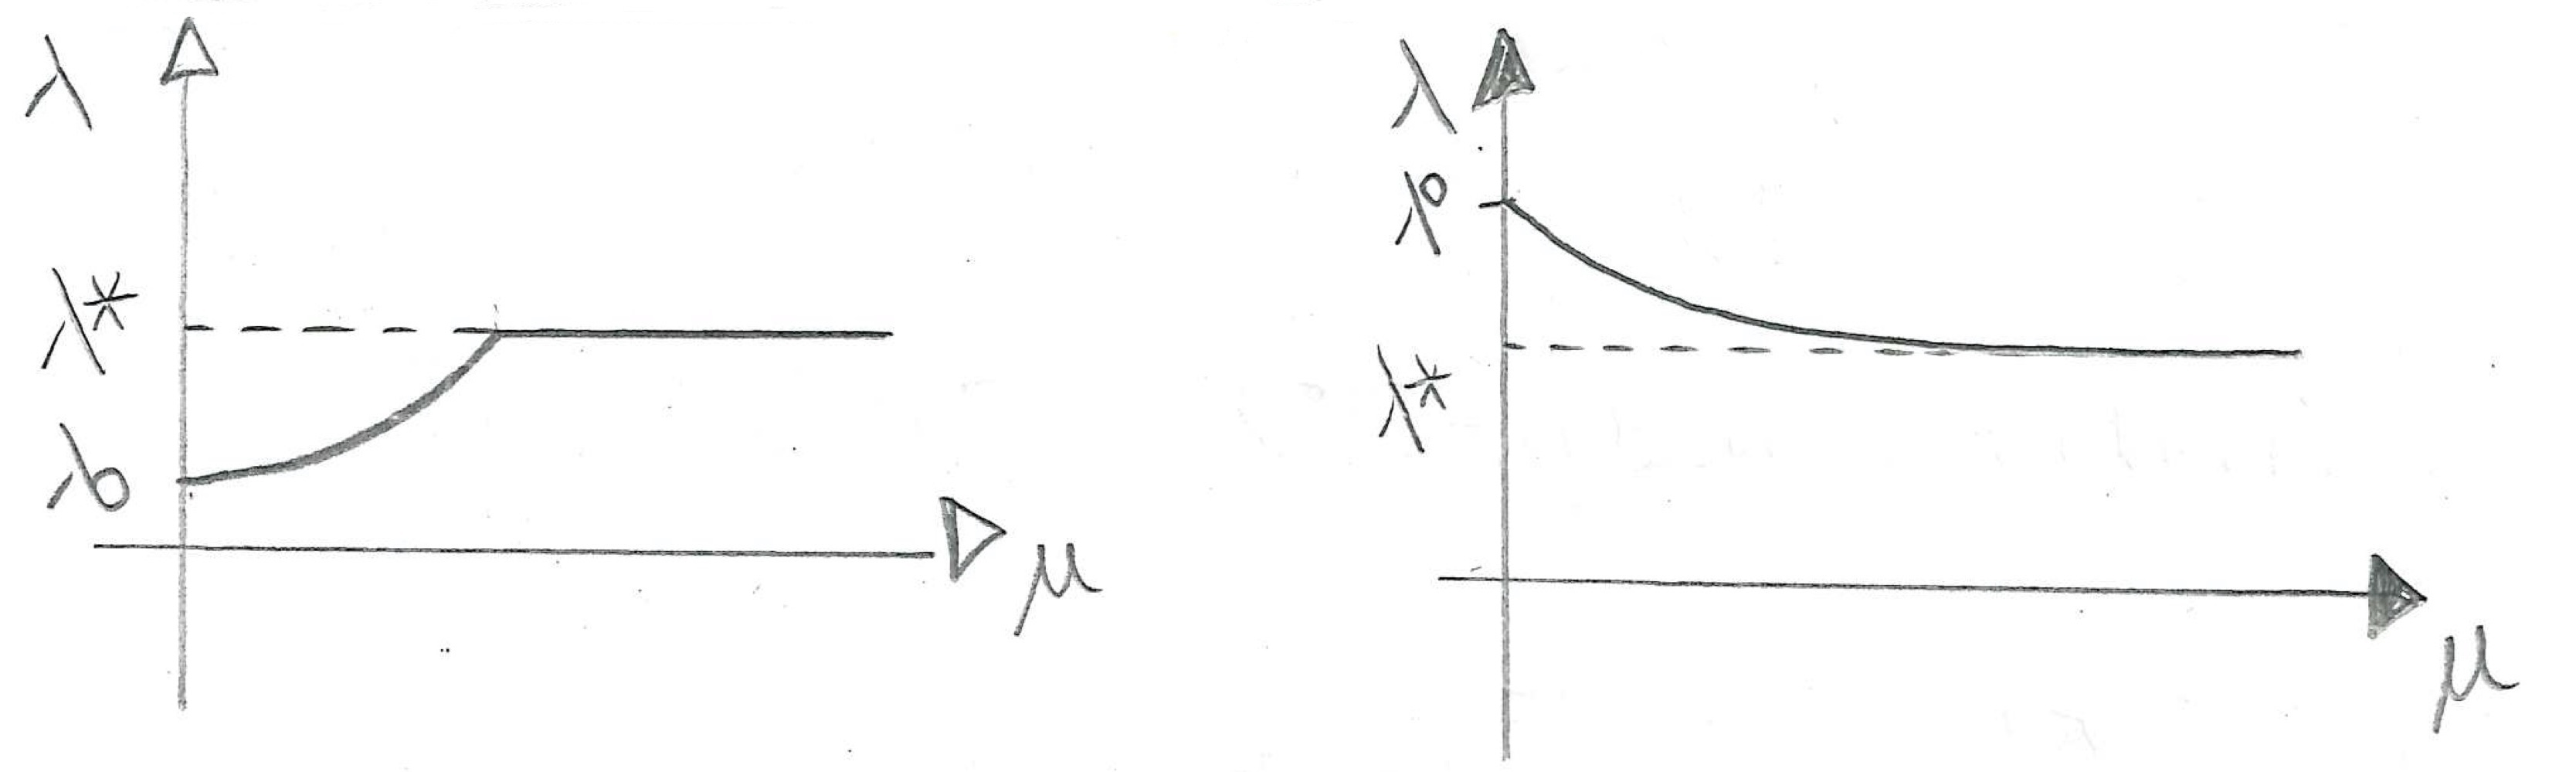
\includegraphics[]{images_ch5/uv_lambdavsmu.jpg}
    
    \item \textbf{Punto fisso infrarosso non banale}\marginnote{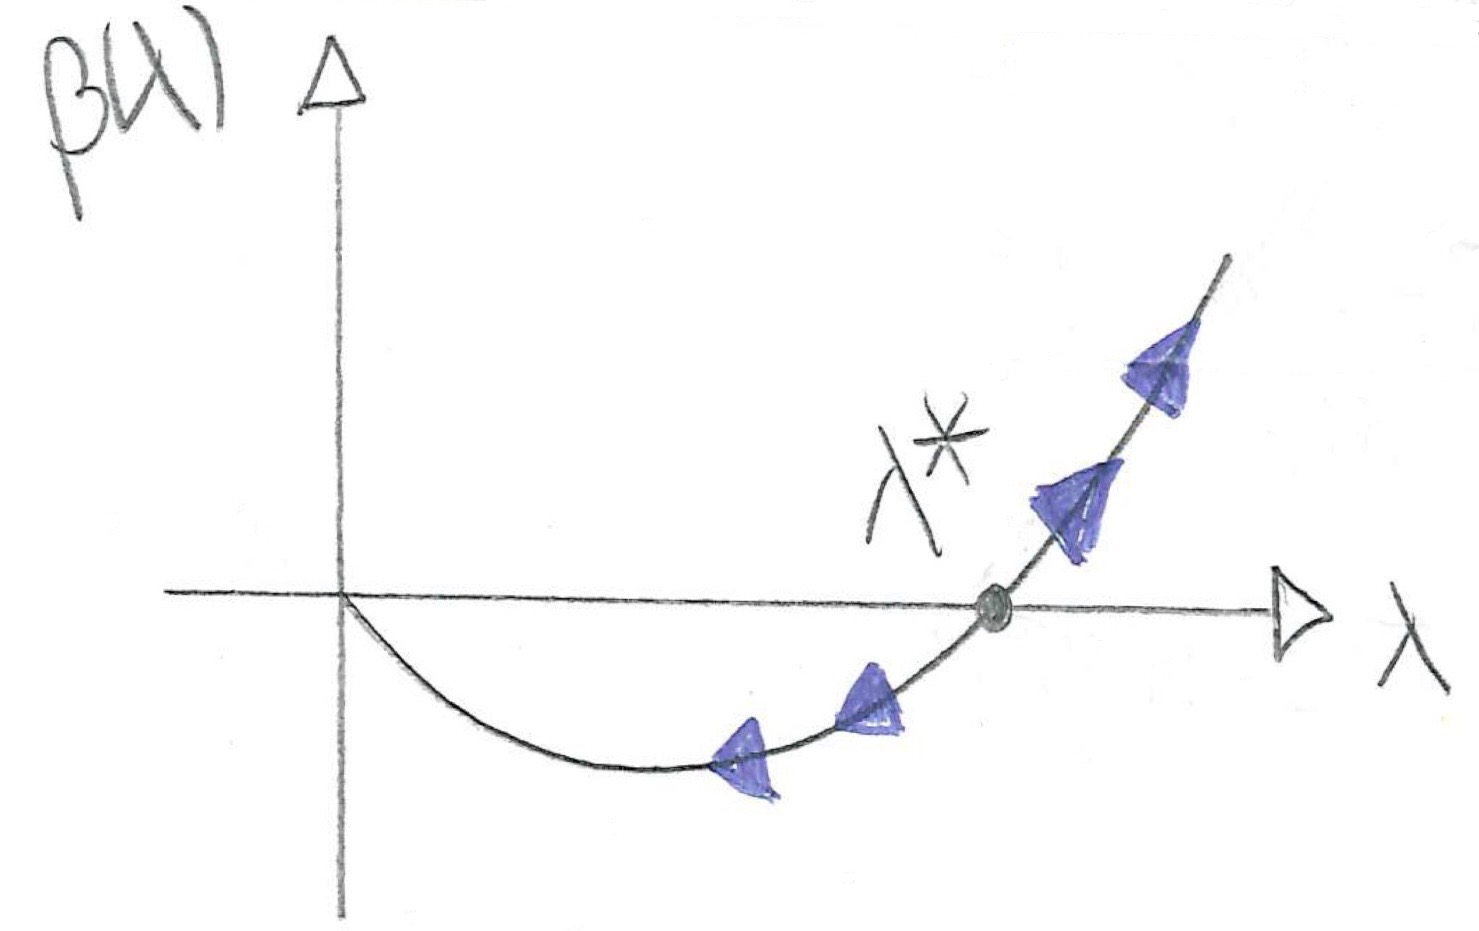
\includegraphics[]{images_ch5/ir_fixed.jpg}\\ Plot schematico di una funzione beta con punto fisso infrarosso. Le frecce blu indicano l'andamento di \(\lambda\) con l'aumentare di $\mu$.}

    Mettiamoci ora nella situazione opposta, anch'essa schematizzata a lato, in cui:
    \begin{align*}
        &\beta(\lambda_\ast) = 0 ~~,~~ \beta'(\lambda_\ast)>0 \\
        &\beta(\lambda) < 0 ~~,~~   \lambda < \lambda_\ast \\
        &\beta(\lambda) > 0 ~~,~~   \lambda > \lambda_\ast
    \end{align*}

    In questo caso, partendo da un certo valore $\lambda_0$ nel regime IR di $\mu$, $\lambda$ tenderà ad allontanarsi da $\lambda_\ast$ con l'aumentare di $\mu$. 

    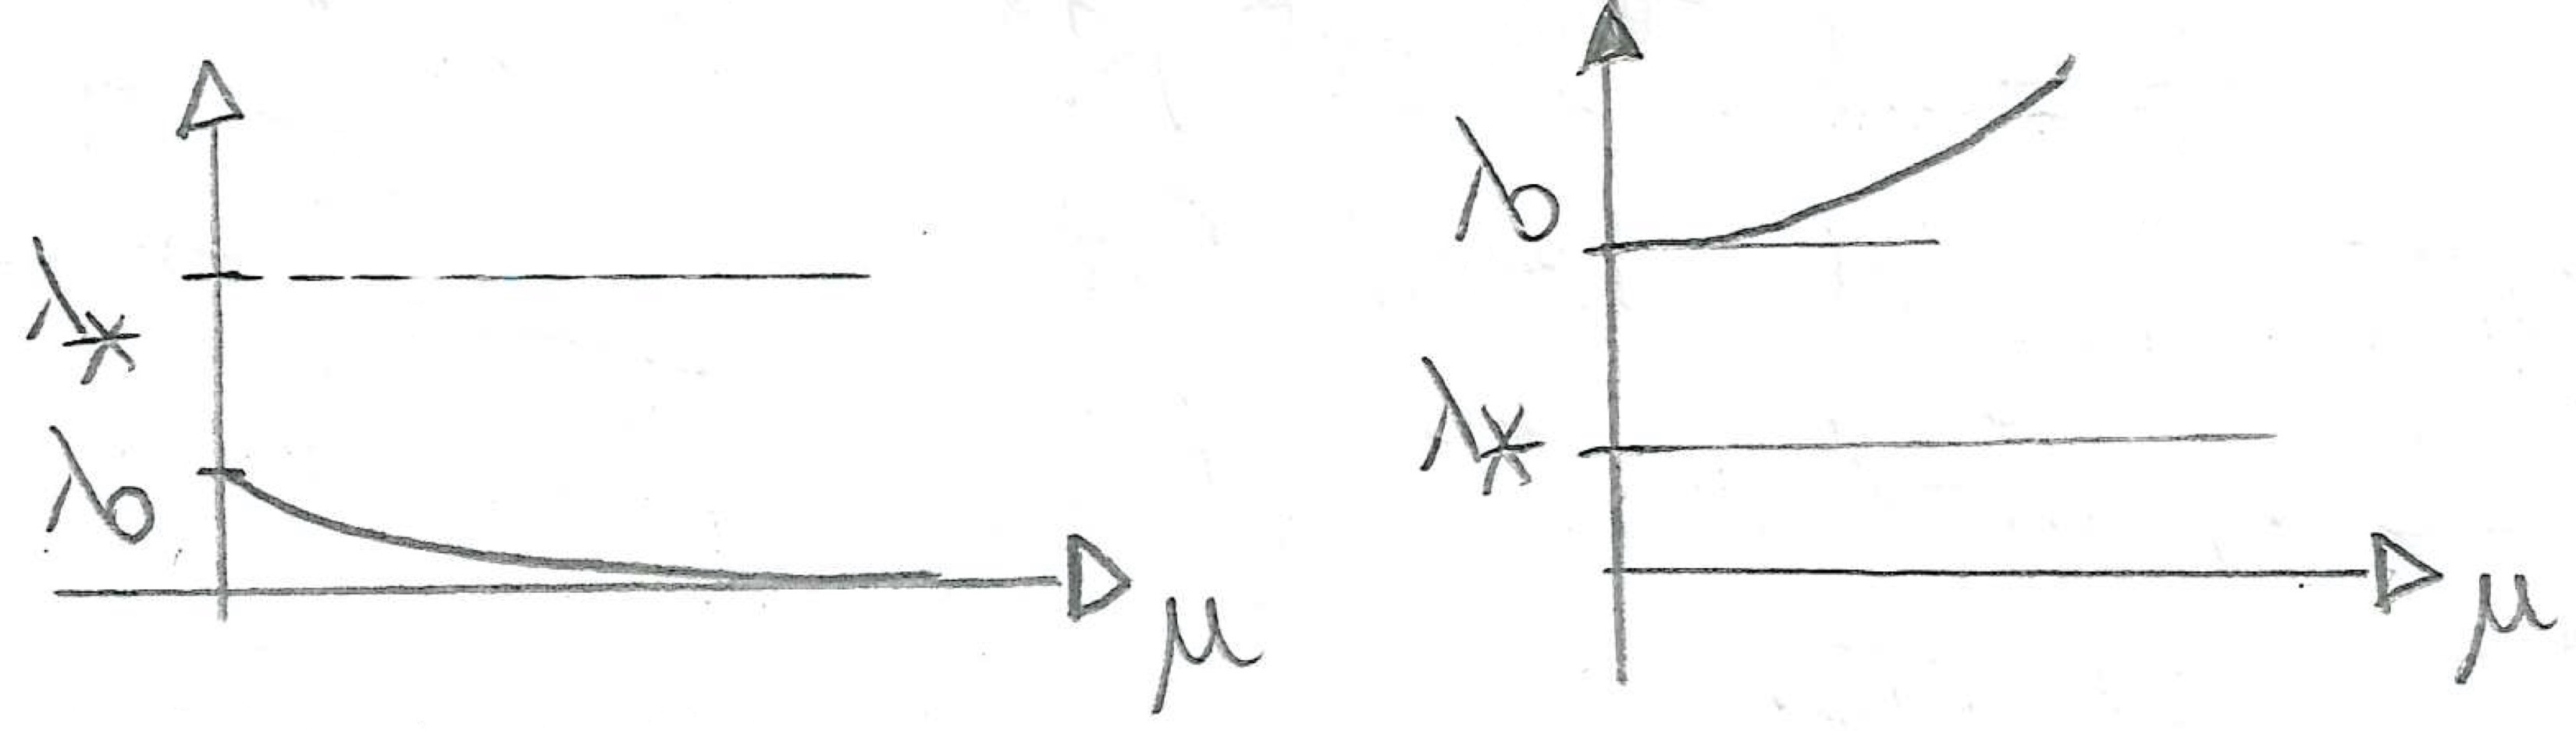
\includegraphics[]{images_ch5/ir_lambdavsmu.jpg}
    
    \marginnote{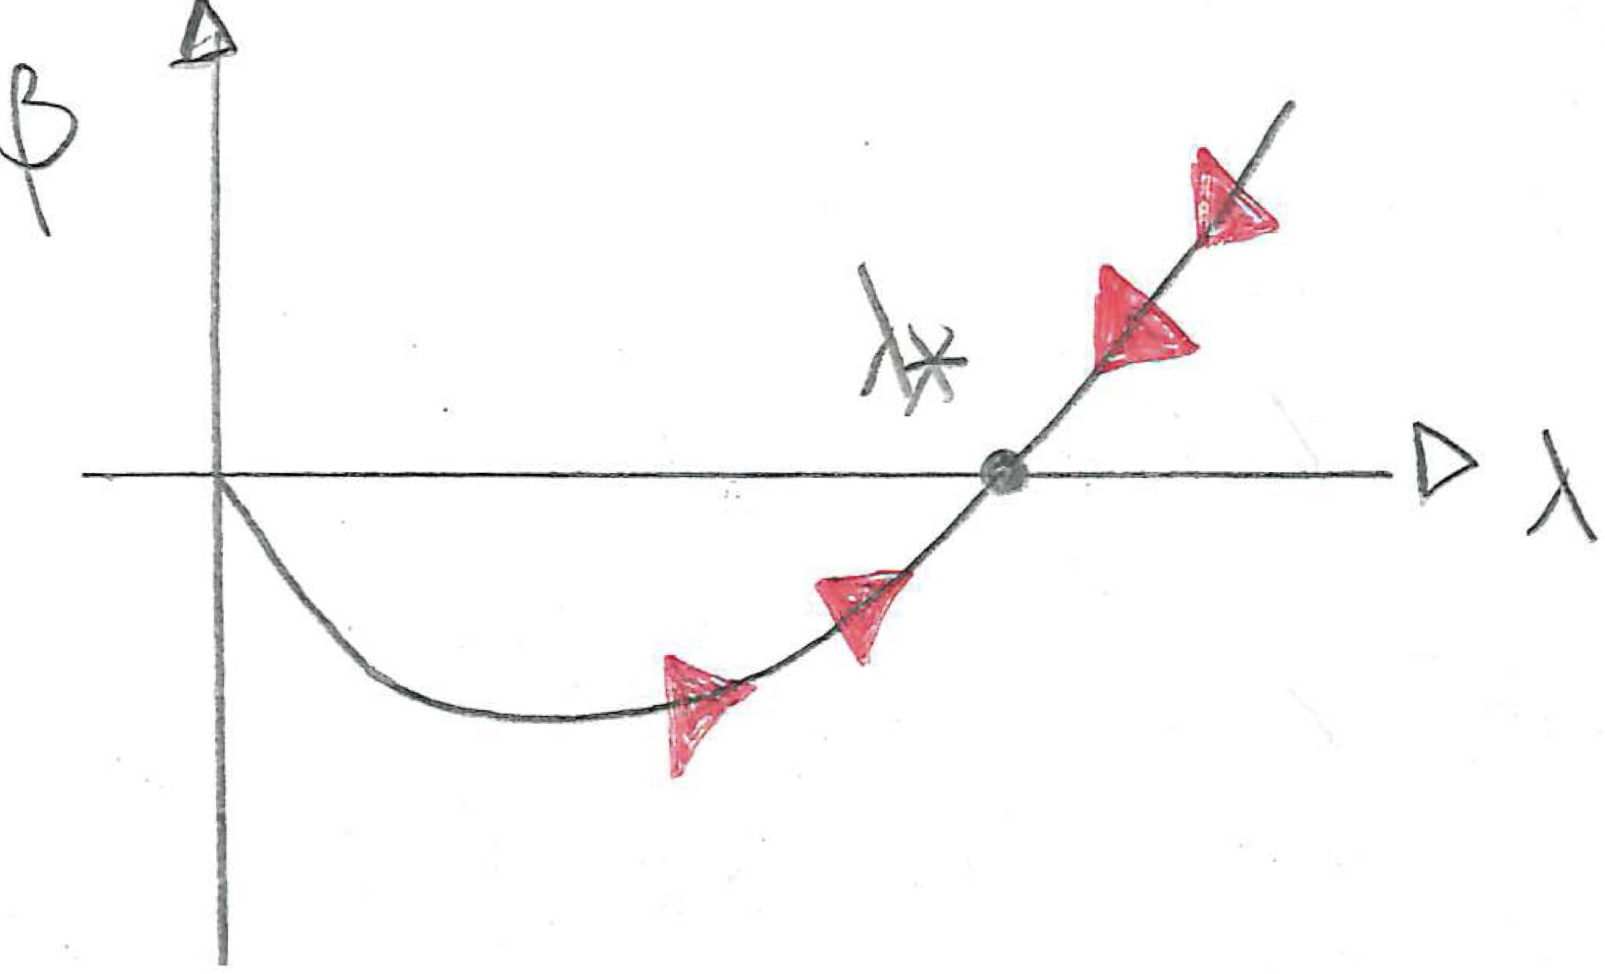
\includegraphics[]{images_ch5/ir_fixed1.jpg}\\ Plot schematico di una funzione beta con punto fisso infrarosso. Le frecce rosse indicano l'andamento di \(\lambda\) con il decrescere di $\mu$.}
    È inoltre interessante interessante analizzare l'andamento di $\lambda$ al decrescere di $\mu$, che è esattamente il contrario rispetto a quello visto poco fa, lo schematizziamo nuovamente a lato, utilizzano frecce di un colore diverso nel grafico \(\beta ~ vs.~ \lambda\).

    Ovviamente, se partiamo da un valore limite \(\lambda_{UV}\) e riduciamo l'energia $\mu$, il flusso del gruppo di rinormalizzazione sarà “diretto” verso $\lambda_\ast$.
    
    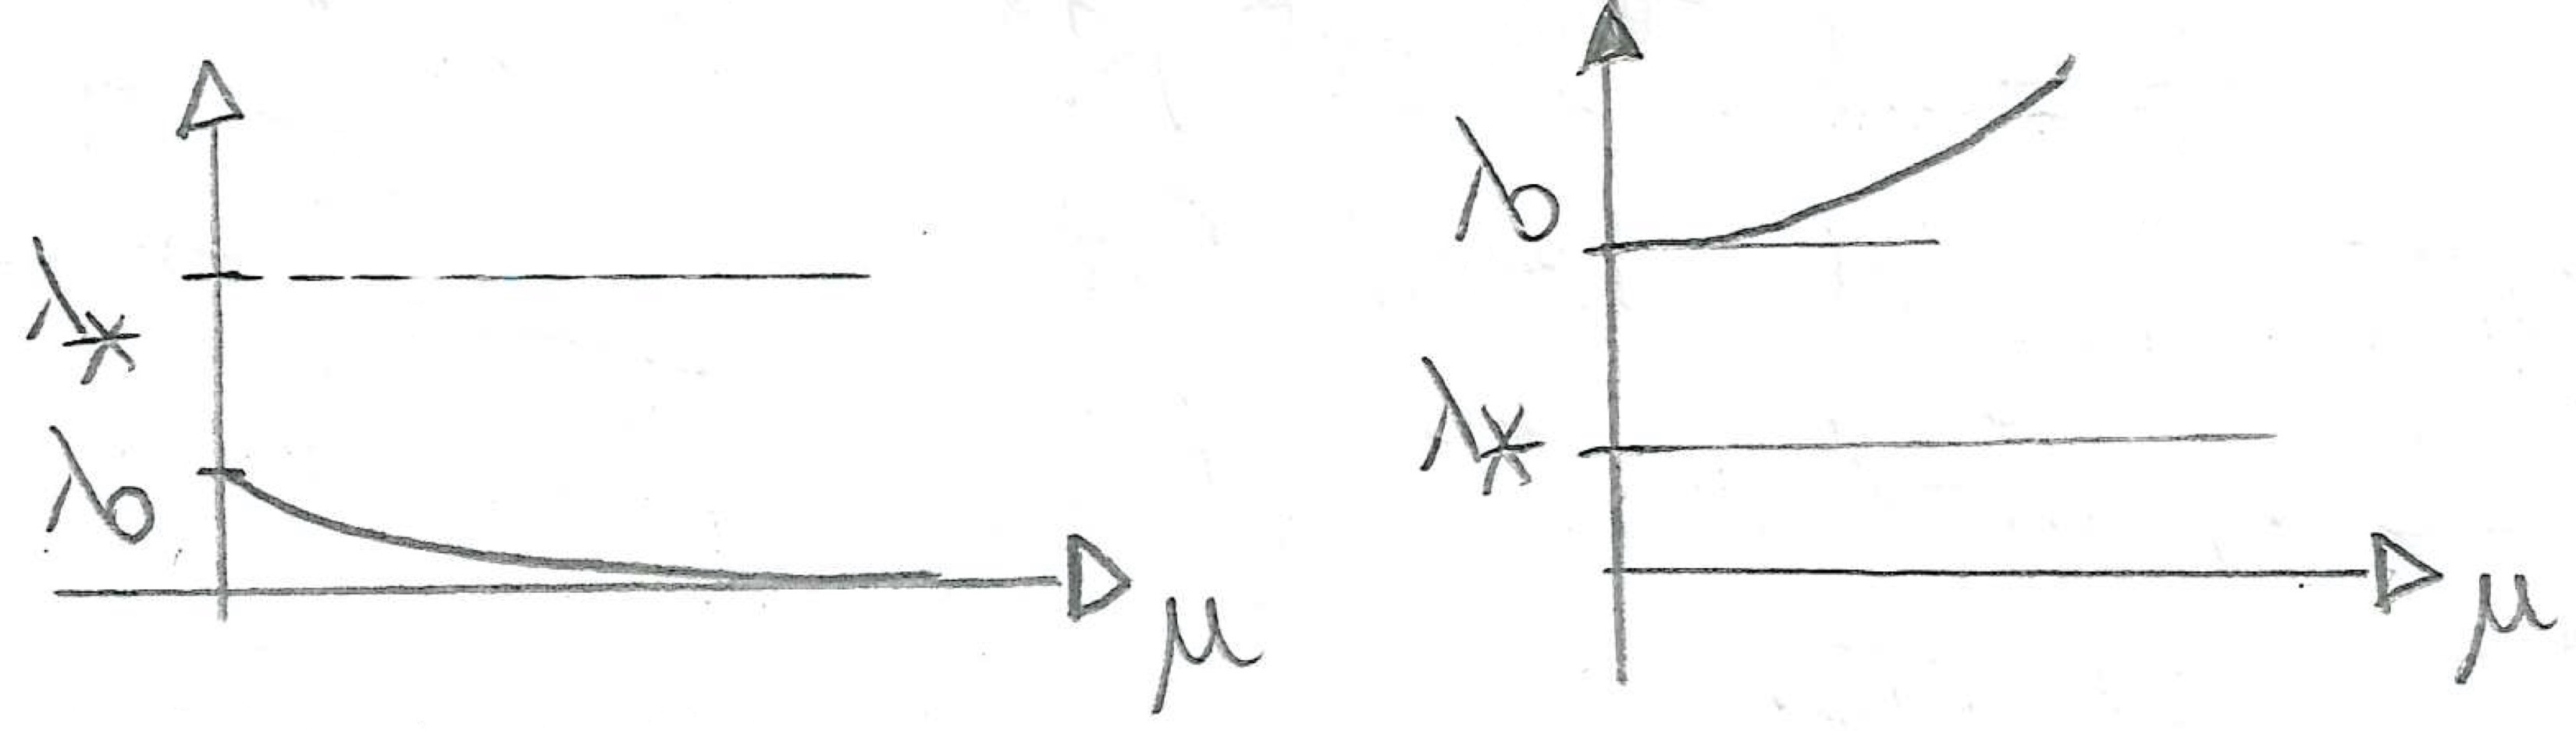
\includegraphics[]{images_ch5/ir_lambdavsmu.jpg}

    Qui $\lambda_\ast$ (con l'asterisco basso) è detto punto fisso infrarosso o punto fisso di \textbf{Wilson-Fisher}.
\end{itemize}

\section{Il Teorema Ottico}
\label{sec:opt_theorem}
Prendiamo nuovamente in considerazione l'equazione l'auto-energia del fotone, ed in particolare la sua parte scalare riportata in equazione (\ref{eq:bar_pi_1loop_fixed}): 
\[
\overline\Pi_\text{1-loop}(q^2) = \frac{e_R^2}{2\pi^2}\int\limits_0^1 dx \,x(1-x)\log{\frac{m^2- x(1-x)q^2}{m^2}}
\]

Precedentemente, trattando lo scattering \(e^-\mu^-\rightarrow e^-\mu^-\) nel canale t in sezione \ref{subsec:ee_mumu_scattering}, abbiamo studiato il caso in cui \(q^2 = - 2|\Vec p|^2(1-\cos\vartheta) < 0\), che rendeva l'argomento del logaritmo sempre positivo.

Studiamo adesso un processo diverso, l'annichilazione \(e^+e^-\rightarrow\mu^+\mu^-\)
\[
\feynmandiagram[horizontal= a to b]{
    i1[particle=$e^+$] --[anti fermion, momentum'=\(p_2\)] a --[anti fermion, edge label=\(p_1\)] i2[particle=$e^-$],
    a --[photon, momentum=$q$] b,
    f1[particle=$\mu^-$] --[anti fermion] b --[anti fermion, momentum'=\(\)] f2[particle=$\mu^+$]}; 
\]
In questo caso l'impulso trasferito tramite il propagatore del fotone è legato all'energia totale nel centro di massa ed è sempre positivo: \(q^2 = (p_1+p_2)^2 = s = 4E^2 >0\). Ciò implica lo sviluppo di una parte immaginaria per il logaritmo presente in \(\overline\Pi_\text{1-loop}(q^2)\).

\paragraph{\textcolor{blue}{Calcolo della parte immaginaria di \(\mathbf{\overline\Pi(q^2)}\).}} Quando abbiamo definito \( \Delta \equiv m^2- x(1-x)q^2\) durante il calcolo degli integrali al loop, abbiamo svolto i calcoli assumendo \(\Delta > 0\). Questo ci ha permesso di effettuare una rotazione di Wick senza alcun impedimento.\marginnote{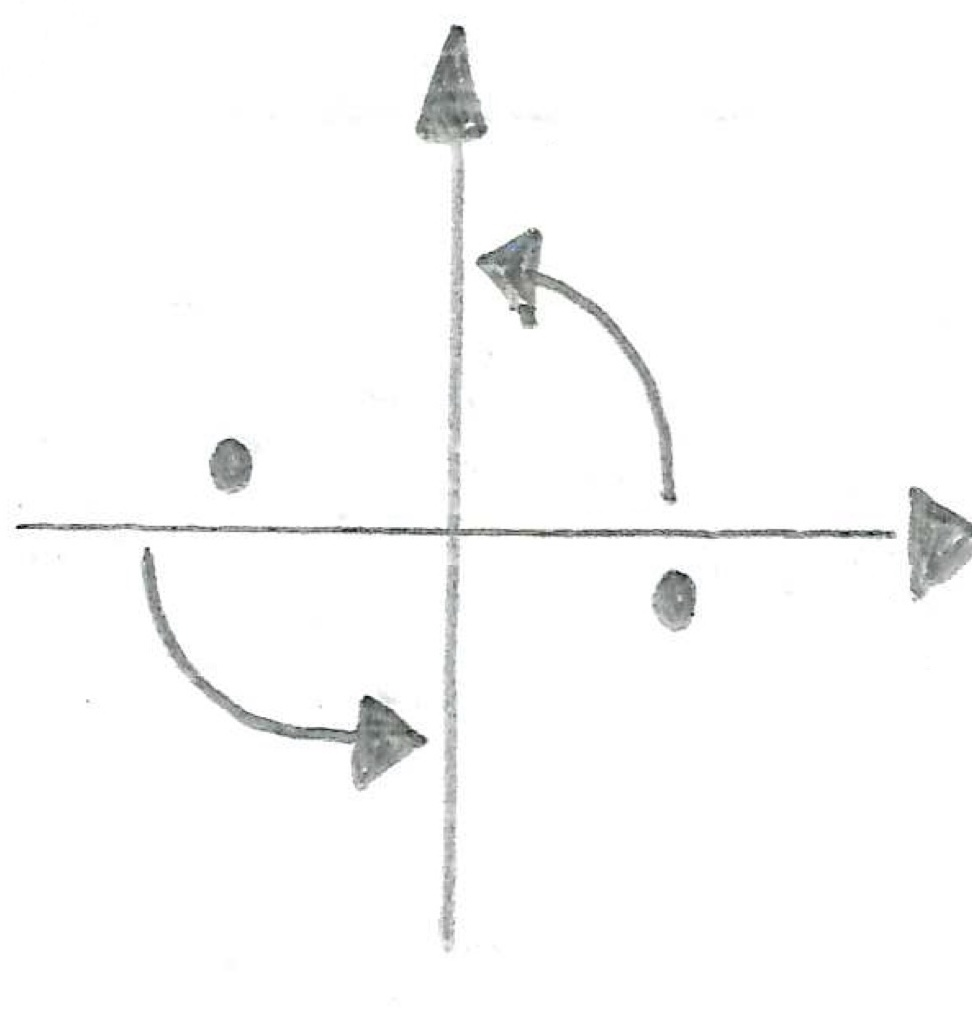
\includegraphics[]{images_ch5/wick_rot_pos.jpg} \\ Schematizzazione della rotazione di Wick effettuata nel caso con $\Delta > 0$. Sono rappresentati anche i poli della funzione integranda.}

Volendo tenere conto della possibilità che $\Delta < 0$, è ugualmente possibile applicare la rotazione di Wick, e la ragione è la seguente: ricordiamo che l'integrale da calcolare è 
\[
\int\frac{d^{\mathsf d -1}\Vec l}{(2\pi)^\mathsf d}\int\limits_{-\infty}^{+\infty}dl^0\, \frac{l^{2n}}{\Big[ \big(l^0\big)^2 - |\Vec{l}|^2 - \Delta + i\varepsilon \Big]^m}
\]
e questo integrale ha chiaramente poli in \(l^0 = \pm \Big[|\Vec{l}|^2 + \Delta - i\varepsilon\Big]^{\nicefrac{1}{2}}\).

La situazione si fa scomoda nel momento in cui $\Delta$ è talmente negativa da rendere \(|\Vec{l}|^2 + \Delta < 0\).

Mettiamoci allora in tale caso estremo ed analizziamo come evolve la struttura dei poli. Possiamo scrivere:
\begin{align*}
    l^0 
    &= \pm \Big[ -\big||\Vec{l}|^2 + \Delta\big| - i\varepsilon \Big]^{\nicefrac{1}{2}} = \pm i\big||\Vec{l}|^2 + \Delta\big|^{\nicefrac{1}{2}} \bigg[ 1 + \frac{i\varepsilon}{\big||\Vec{l}|^2 + \Delta\big|} \bigg]^{\nicefrac{1}{2}}\\
    & \approx \pm \Big[i\big||\Vec{l}|^2 + \Delta\big|^{\nicefrac{1}{2}} - \varepsilon \Big]
\end{align*}
\marginnote{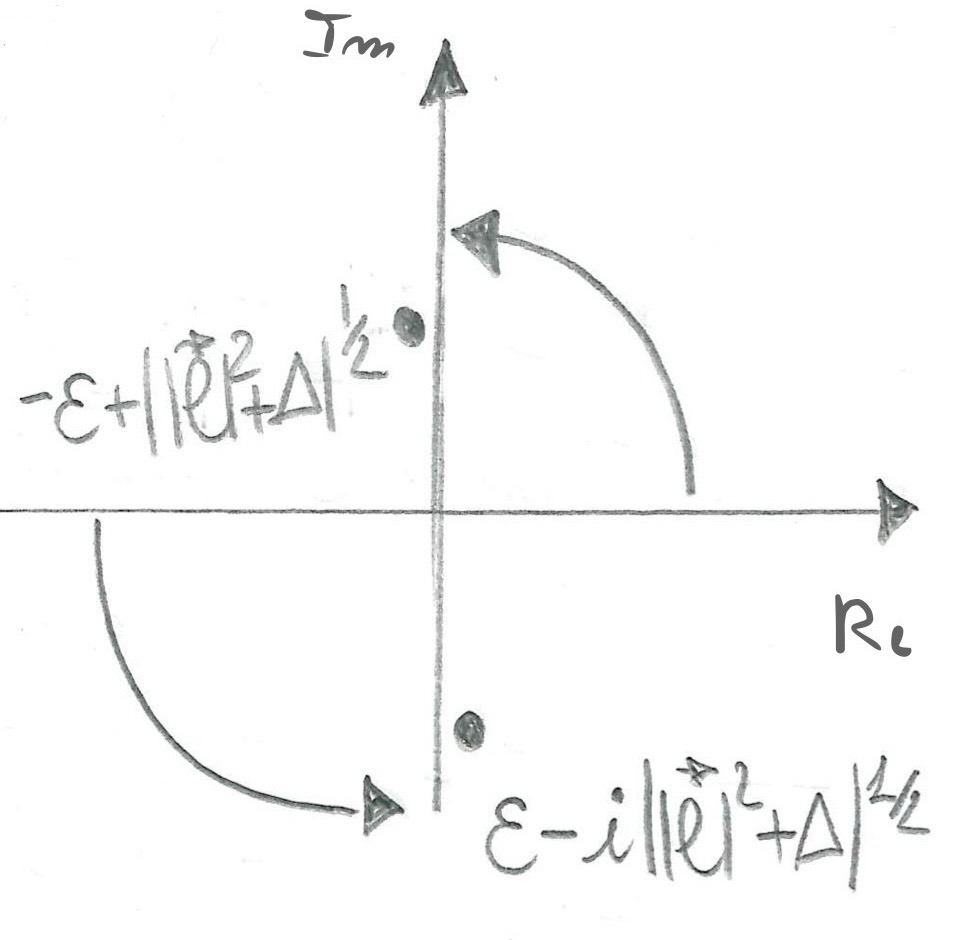
\includegraphics[]{images_ch5/wick_rot_neg.jpg}\\ Schematizzazione della rotazione di Wick effettuata nel caso con $\Delta < 0$. Sono rappresentati anche i poli della funzione integranda.}

Dove nell'ultimo passaggio abbiamo effettuato un'espansione di Taylor sulla radice, riassorbendo il denominatore di $\varepsilon$ in $\varepsilon$ stesso.

In questo caso, i poli sono vicini all'asse immaginario: possiamo ancora ruotare il cammino di integrazione, ma ci conviene mantenere la notazione comprensiva di \(i\varepsilon\), i.e. \(\Delta \rightarrow \Delta - i\varepsilon\). Scriviamo allora:
\[
\overline\Pi_\text{1-loop}(q^2) = \frac{e_R^2}{2\pi^2}\int\limits_0^1 dx \,x(1-x)\log{\bigg[\frac{\Delta - i\varepsilon}{m^2}\bigg]}
\]

Sia adesso \( z = \Delta - i\varepsilon \), sappiamo che \(\log z = \log|z| + i\arg z\). Abbiamo quindi ancora il logaritmo con argomento positivo, che fornisce la stessa fenomenologia già discussa precedentemente (e.g. le correzioni alla carica elettrica), ma abbiamo anche una parte immaginaria, quella che vogliamo calcolare.

\marginnote{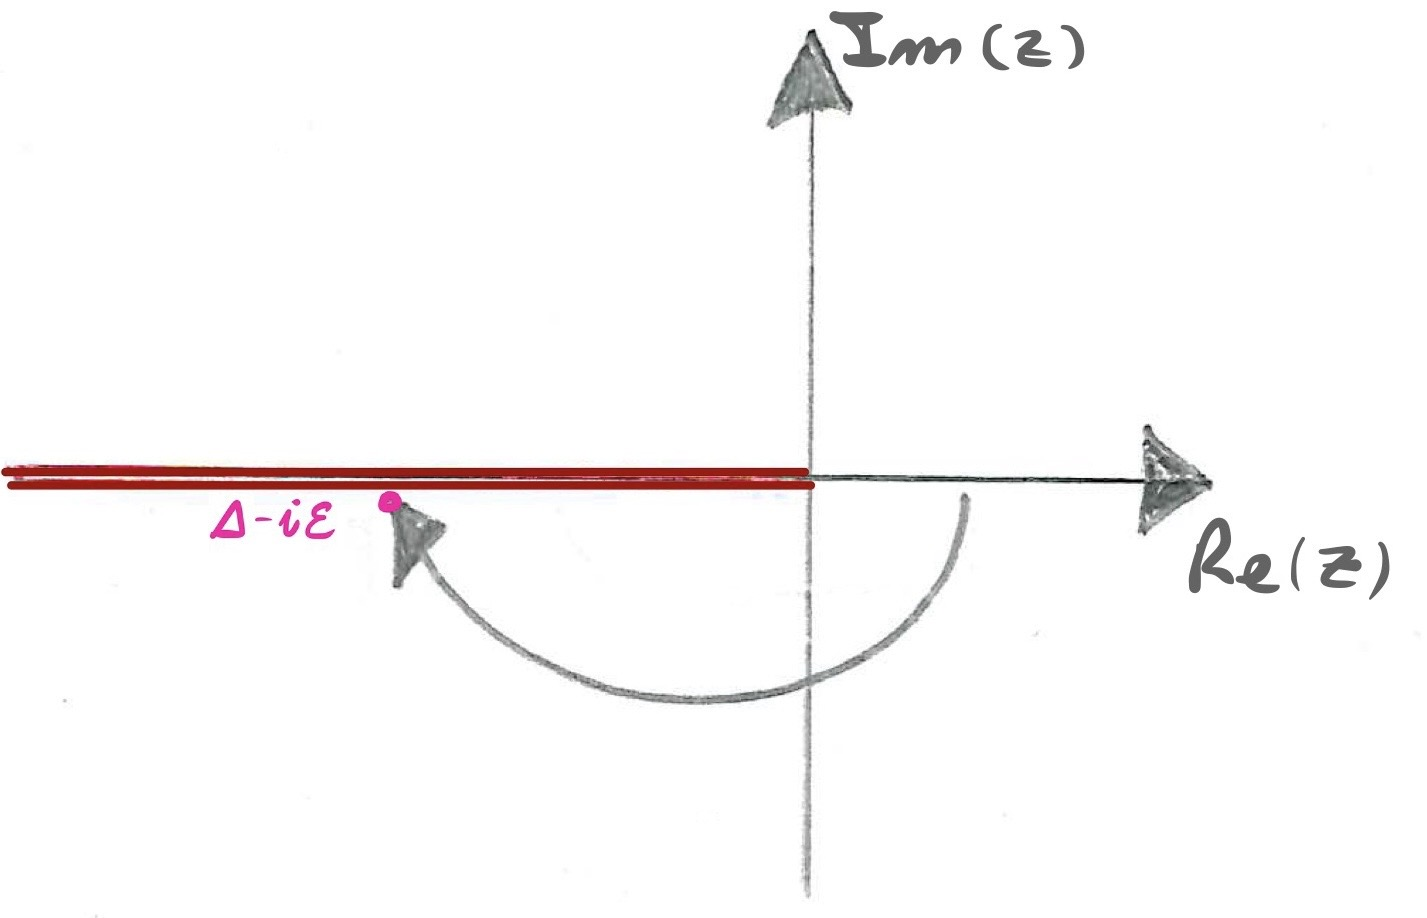
\includegraphics[]{images_ch5/argz.jpg}}
Dobbiamo tagliare lungo l'asse reale negativo, dove il logaritmo non è definito, ed essendo \(z < 0\) ma leggermente shiftato verso il basso per via del \(-i\varepsilon\), perciò dobbiamo valutare il suo argomento “da sotto”, come schematizzato a lato.

Di conseguenza, ci accorgiamo che \(\boxed{\arg z = -\pi}\).

Vogliamo adesso studiare sotto quale condizione $z$, che dipende da $x$, sia negativo. Stiamo considerando il caso \(\Delta = m^2 - x(1-x)q^2\leq 0\), e risolvendo l'equazione \(\Delta = 0\) troviamo gli estremi dell'intervallo di $x$ per cui vale la nostra condizione iniziale. In sintesi:

\begin{align*}
    m^2 - x(1-x)q^2\leq 0 ~~ &\forall ~ x \in [x_-, x_+], \\
    \text{con } &x_\pm \equiv \frac{1\pm\sqrt{1-\nicefrac{4m^2}{q^2}}}{2}
\end{align*}

Ci accorgiamo, inoltre, del fatto che \(x(1-x)\) nell'intervallo \(x\in[0,1]\) si annulla agli estremi ed ha massimo \(\nicefrac{1}{4}\) per \(x=\nicefrac{1}{2}\). Abbiamo quindi
\[
m^2-\frac{q^2}{4} \leq m^2 - x(1-x)q^2 \leq 0 \Rightarrow \boxed{q^2\geq 4m^2}
\]

La parte immaginaria che stiamo cercando è quindi:

\[
i\Im \overline{\Pi}(q^2) = \overbrace{i(-\pi)}^{i\arg z} \frac{e^2}{2\pi^2}\int\limits_{x_-}^{x_+} dx \,x(1-x)
\]

Prendendo per buono che \(\int\limits_{x_-}^{x_+} dx \,x(1-x) = \frac{1}{6q^2}(2m^2+q^2)\sqrt{1-\nicefrac{4m^2}{q^2}}\), arriviamo al risultato finale:
\begin{equation}
    \boxed{
    \Im \overline{\Pi}(q^2) = -\frac{e^2}{12\pi}\bigg(1 + \frac{2m^2}{q^2}\bigg)\sqrt{1-\frac{4m^2}{q^2}}
    }
    \label{eq:barPi_imaginarypart}
\end{equation}
generata quando \(q^2 \geq m^2\). \textcolor{blue}{\qed}

A questo punto è facile notare una certa familiarità in questa espressione, in particolare nel fattore \(\sqrt{1-\nicefrac{4m^2}{q^2}}\). Questo infatti è identico al fattore di spazio delle fasi\footnote{Anche detto \textit{two-particle LIPS} (= Lorentz Invariant Phase-Space).} per lo stato finale a due particelle di massa $m$ ed energia del centro di massa $\sqrt{q^2}$. Non può essere una coincidenza, ed infatti non lo è: \textbf{è una conseguenza dell'unitarietà della matrice $S$}, e si rispecchia nel teorema ottico.

Per muoverci verso l'enunciato del teorema ottico, consideriamo l'operatore di scattering, i.e. la matrice $S$, che generalmente useremo dentro il sandwich $\langle f | \cdots | i \rangle$. In particolare siamo interessati all'elemento di matrice generato dall'espansione al prim'ordine:
\[
S = \mathbb 1 + iT ~~,~~ \langle f | T | i \rangle = (2\pi)^4\delta(p_f-p_i)\mathscr M_{fi}
\]
Dall'unitarietà \(S^\dagger S = \mathbb 1\) si trova, sostituendo l'espansione della matrice $S$:
\[
T-T^\dagger = iT^\dagger T
\]

Adesso prendiamo il sandwich di quest'ultima equazione, ricordando che \(\langle f | T^\dagger | i \rangle = \big(\langle i | T | f \rangle \big)^\ast\). Quello che troviamo è:

\[
\langle f | T | i \rangle - \big(\langle i | T | f \rangle \big)^\ast = i \langle f | T^\dagger T | i \rangle 
\]

\begin{nota}
    \textbf{(Relazione di Completezza.)}\\
    Richiamiamo la relazione di completezza nello spazio di Hilbert multi-particellare della teoria considerata, in questo caso la QED con solo elettroni e fotoni, per semplicità:
    \begin{equation}
        \mathbb 1 = \sum_X \sumint d\Pi_X |X\rangle \langle X|
        \label{eq:completeness_relation}
    \end{equation}

    dove \(|X\rangle\) rappresenta un qualsiasi stato multi-particellare.

    Prendiamo ad esempio lo stato con un singolo elettrone con impulso $\Vec p$ e polarizzazione $s$, i.e. \(|e^-(\Vec{p}, s)\rangle \). Questo stato contribuisce alla relazione di completezza nel modo seguente:
    \[
    \mathbb 1 = \cdots + \underbrace{\sum_s \int \frac{d^3\Vec{p}}{(2\pi)^3 2E_p}}_{\sumint d\Pi_X} |e^-(\Vec{p}, s)\rangle \langle e^-(\Vec{p}, s)| + \cdots
    \]
    da cui si definisce l'integrale sommato per uno stato di singola particella, che corrisponde alla somma sui possibili gradi di libertà dello stato \(|X\rangle\) considerato, siano essi discreti (come lo spin) o continui (come l'impulso).

    Ovviamente alla somma contribuiranno anche stati con più di una particella, e.g. \(|e^-(\Vec{p}, s) \gamma(\Vec k, \lambda) \rangle \), ed in tal caso in \(\sumint d\Pi_X\) vengono inclusi tutti gli integrali (su $\Vec{p}$ e $\Vec{k}$) e le somme (su $s$ e $\lambda$).
\end{nota}

A questo punto inseriamo la relazione di completezza (\ref{eq:completeness_relation}) nell'equazione a cui eravamo arrivati, per mezzo di una identità tra \(T^\dagger T\) nel membro a destra, ottenendo:
\begin{align*}
    \langle f | T | i \rangle - \big(\langle i | T | f \rangle \big)^\ast 
    & = i \sum_X \sumint d\Pi_X \langle f | T^\dagger |X\rangle \langle X| T | i \rangle \\
    & = i \sum_X \sumint d\Pi_X \big(\langle X | T |f\rangle\big)^* \langle X| T | i \rangle
\end{align*}

In termini di ampiezze di scattering:

\begin{align*}
    (2\pi)^4\delta(p_f-p_i) &\mathscr M_{fi} - (2\pi)^4\delta(p_i-p_f) \mathscr M^*_{if} = \\
    &= i \sum_X \sumint d\Pi_X (2\pi)^4\delta(p_X-p_f)\mathscr M^*_{Xf} (2\pi)^4\delta(p_X-p_i)\mathscr M_{Xi}
\end{align*}

Possiamo riscrivere il prodotto delle $\delta$ nel RHS avvalendoci del fatto che la seconda delta forza $p_X=p_i$ nella prima, i.e. 
\[\delta(p_X-p_f)\delta(p_X-p_i) = \delta(p_i-p_f)\delta(p_X-p_i)\]
Questo ci permette di raccogliere le $\delta$ a sinistra, che di fatto sono uguali, e semplificarle con quella a destra.

Siamo ora pronti ad enunciare il teorema ottico generalizzato, e lo facciamo adottando la notazione \(\mathscr M_{fi} \equiv \mathscr M(i\rightarrow f)\), esplicitando gli stati iniziali e finali.

Inoltre ricordiamo che \(p_i\) e \(p_x\) rappresentano rispettivamente i 4-impulsi totali degli stati \(|i\rangle\) ed  \(|X\rangle\).

\begin{theorem}
    \textbf{(Teorema Ottico Generalizzato.)}
    \begin{equation}
        \begin{aligned}
             \mathscr M(i\rightarrow f)& -  \mathscr M(f\rightarrow i)^* =\\&= i \sum_X \sumint d\Pi_X (2\pi)^4\delta(p_X-p_i)\mathscr M(f\rightarrow X)^* \mathscr M(i \rightarrow X)
        \end{aligned}
    \end{equation}
    \label{th:generalized_optical_theorem}
\end{theorem}

Se ora consideriamo \(|i\rangle = |f\rangle = |\alpha\rangle\), ricordando che \(\mathscr M_{\alpha\alpha} -  \mathscr M_{\alpha\alpha}^* = 2i\Im \mathscr M_{\alpha\alpha}\), possiamo riscriverlo nel seguente modo:

\begin{theorem}
    \textbf{(Teorema Ottico.)}
    \begin{equation}
         2\Im\mathscr M(\alpha \rightarrow \alpha) = \sum_X \sumint d\Pi_X (2\pi)^4\delta(p_X-p_\alpha) \big|\mathscr{M}(\alpha \rightarrow X )\big|^2
    \end{equation}
    \label{th:optical_theorem}
\end{theorem}
Il teorema ottico vale in maniera non perturbativa ed inoltre è valido ad ogni ordine in teoria delle perturbazioni.

Questa affermazione ha un significato ben preciso. Notiamo infatti come a destra abbiamo un'ampiezza al quadrato, mentre a sinistra abbiamo semplicemente un'ampiezza.

\begin{example}
    A titolo di esempio, consideriamo la teoria scalare
    \[
    \mathscr L = \frac{1}{2} \big( \partial_\mu \phi\big)\big( \partial^\mu \phi\big) -\frac{m^2}{2}\phi^2 - \frac{\lambda}{4!} \phi^4
    \]
    con interazione: 
    \(\feynmandiagram[small, horizontal=i1 to f1, scale=0.6, baseline=(v.base), layered layout]{
        {i1,i2} --[scalar] v[dot] --[scalar] {f1,f2},
        %{[same layer] a,b}
        };\) .

    Prendiamo un semplice stato con due particelle scalari, i.e. senza spin, \(|\alpha\rangle = |\Vec p_1,\Vec p_2\rangle\). 

    Concentriamoci sul RHS del teorema ottico: in linea di principio dovremmo sommare su tutti i possibili stati multi-particellari, ma possiamo troncare la serie all'ordine $\mathscr O (\lambda^2)$, includendo quindi a sinistra solo diagrammi del tipo sopra, interpretando le 4 linee come due particelle per lo stato iniziale e due per il finale. Se andiamo a scrivere il teorema ottico, al LHS dovremmo matchare l'ordine di interazione prodotto dal modulo quadro al RHS, ad esempio:
    \begin{align*}
        2\Im\Bigg[
        &\feynmandiagram[small, scale=0.9, horizontal=v1 to v2, baseline=(v1.base)]{
                {i1[label = \(p_1\)],i2[label = below:\(p_2\)]} --[charged scalar ] v1[dot] --[scalar, half left] v2[dot] --[scalar, half left] v1,
                v2 --[charged scalar] {f1[label = below:\(p_2\)],f2[label = \(p_1\)]}
        };
        \Bigg] =\\
        & = \int\frac{d^3\Vec{k_1}}{(2\pi)^3 2E_{k_1}}\int\frac{d^3\Vec{k_2}}{(2\pi)^3 2E_{k_2}} (2\pi)^4\delta(k_1+k_2-p_1-p_2) 
        \Bigg|~
        \feynmandiagram[small, horizontal=i1 to f1, scale=0.8, baseline=(v.base), layered layout]{
        {i1[label=\(p_1\)],i2[label=below:\(p_2\)]} --[charged scalar] v[dot] --[charged scalar] {f1[label=\(k_1\)],f2[label=below:\(k_2\)]},
        };~
        \Bigg|^2
    \end{align*}
    Apprendiamo quindi che \textbf{l'unitarietà connette in maniera inestricabile il tree-level ed i loop}! In particolare, la parte immaginaria di un'ampiezza ad un loop è determinata da un processo al tree-level.
\end{example}

In luce di quanto appena visto, torniamo al nostro problema principale e consideriamo il teorema ottico in QED con soli fotoni ed elettroni. Prendiamo uno stato iniziale \(|\alpha\rangle \equiv |e^-(\Vec p_1, s_1)  e^+(\Vec p_2, s_2)\rangle\) e applichiamo il teorema ottico all'ordine minore in teoria delle perturbazioni, i.e. consideriamo solo gli stati finali a due particelle, in altre parole lo scattering BhaBha.
\begin{align*}
    \Bigg|
    \feynmandiagram[small, horizontal=v1 to v2, baseline=(v1)]{
            i1[label = below:\(p_1\)] --[anti fermion, momentum'=\( \)] v1[dot] --[anti fermion] i2[label = \(p_2\)],
            v1 --[photon] v2[dot],
            v2 --[anti fermion, momentum'=\( \)] f1[label = below:\(k_2\)]  ,
            v2 -- [fermion] f2[label = \(k_1\)],
    };
    -
    \begin{tikzpicture}[baseline=\plusheight]
        \begin{feynman}
            \vertex[small, dot, label=$p_1$] (a) at (-1.2,0.7) {};
            \vertex[small, dot, label=$k_1$] (b) at (1.2,0.7) {};
            \vertex[small, dot] (i1) at (0,0.5) {};
            \vertex[small, dot] (i2) at (0,-0.5) {};
            \vertex[small, dot, label=below:$p_2$] (c) at (-1.2,-0.7) {};
            \vertex[small, dot, label=below:$k_2$] (d) at (1.2,-0.7) {};
            \diagram*[small]{
                (a) --[fermion] (i1) --[fermion] (b),
                (i1) --[photon] (i2),
                (c) --[anti fermion, momentum'] (i2) --[anti fermion, momentum'] (d)
            };
        \end{feynman}
    \end{tikzpicture}
    \Bigg|^2 \sim \mathscr O(e^4)
\end{align*}

A questo punto, ragionando sul LHS del teorema ottico, abbiamo bisogno di ampiezze \(|\alpha\rangle \rightarrow |\alpha\rangle\) dello stesso ordine, i.e. $\mathscr O(e^4)$, quindi abbiamo bisogno di loop nei diagrammi.

Ci aspettiamo inoltre che questi loop abbiano una parte immaginaria diversa da zero, in modo da matchare il corrispondente contributo al tree-level dovuto al BhaBha scattering.

Volendo scrivere il teorema ottico in maniera diagrammatica (e schematica), sviluppiamo il modulo quadro a destra, ottenendo:
% Qui c'è il teorema ottico compresso
\begin{align*}
&\begin{aligned}
    2\Im\Bigg[&
    \begin{tikzpicture}[baseline=\plusheight]
        \begin{feynman}
            \vertex (i1) at (-1,0.5) {};
            \vertex (i2) at (-1,-0.5) {};
            \vertex[small, dot] (w) at (-0.5,0) {};
            \vertex[small, dot] (x) at (0,0) {};
            \vertex[small, dot] (y) at (0.5,0) {};
            \vertex[small, dot] (z) at (1,0) {};
            \vertex (f1) at (1.5,0.5) {};
            \vertex (f2) at (1.5,-0.5) {};
            \diagram*[small,scale=0.7]{
                {(i1),(i2)} -- (w) --[photon] (x) --[half left] (y) --[half left] (x),
                (y) --[photon] (z) -- {(f1),(f2)}
            };
        \end{feynman}
    \end{tikzpicture}
    +
    \begin{tikzpicture}[baseline=\plusheight]
        \begin{feynman}
            \vertex (a) at (-1,0.5) {};
            \vertex (b) at (1,0.5) {};
            \vertex[small, dot] (u1) at (-0.3,0.5) {};
            \vertex[small, dot] (d1) at (-0.3,-0.5) {};
            \vertex[small, dot] (u2) at (0.3,0.5) {};
            \vertex[small, dot] (d2) at (0.3,-0.5) {};
            \vertex (c) at (-1,-0.5) {};
            \vertex (d) at (1,-0.5) {};
            \diagram*[small,scale=0.7]{
                (a) -- (u1) -- (u2)-- (b),
                (u1) --[photon] (d1),
                (u2) --[photon] (d2),
                (c) -- (d1) -- (d2) -- (d)
            };
        \end{feynman}
    \end{tikzpicture}
    +
    \begin{tikzpicture}[baseline=\plusheight]
        \begin{feynman}
            \vertex (i1) at (-1,0.5) {};
            \vertex (i2) at (-1,-0.5) {};
            \vertex[small, dot] (x) at (-0.5,0.25) {};
            \vertex[small, dot] (y) at (-0.5,-0.25) {};
            \vertex[small, dot] (a) at (0,0) {};
            \vertex[small, dot] (b) at (1,0) {};
            \vertex (f1) at (2,0.5) {};
            \vertex (f2) at (2,-0.5) {};
            \diagram*[small,scale=0.7]{
                (i1) -- (x) -- (a) -- (y) --[photon] (x),
                (i2) -- (y),
                (a) --[photon] (b) -- {(f1),(f2)}
            };
        \end{feynman}
    \end{tikzpicture}
    +\\
    &+
    \begin{tikzpicture}[baseline=\plusheight]
        \begin{feynman}
            \vertex (i1) at (-1,0.5) {};
            \vertex (i2) at (-1,-0.5) {};
            \vertex[small, dot] (a) at (0,0) {};
            \vertex[small, dot] (b) at (1,0) {};
            \vertex[small, dot] (x) at (1.5,0.25) {};
            \vertex[small, dot] (y) at (1.5,-0.25) {};
            \vertex (f1) at (2,0.5) {};
            \vertex (f2) at (2,-0.5) {};
            \diagram*[small,scale=0.7]{
                {(i1),(i2)} -- (a),
                (a) --[photon] (b) -- (x) --[photon] (y) -- (b),
                (x) -- (f1),
                (y) -- (f2)
            };
        \end{feynman}
    \end{tikzpicture}
    \Bigg] =
\end{aligned}\\
&\begin{aligned}
    = \sumint \Bigg[~
    &\Bigg|
    \begin{tikzpicture}[baseline=\plusheight]
        \begin{feynman} % s-channel
            \vertex (i1) at (-1,0.5) {};
            \vertex (i2) at (-1,-0.5) {};
            \vertex[small, dot] (x) at (-0.5,0) {};
            \vertex[small, dot] (y) at (0.5,0) {};
            \vertex (f1) at (1,0.5) {};
            \vertex (f2) at (1,-0.5) {};
            \diagram*[small,scale=0.7]{
                {(i1),(i2)} -- (x) --[photon] (y) -- {(f1),(f2)}
            };
        \end{feynman}
    \end{tikzpicture}
    \Bigg|^2
    +
    \Bigg| %
    \begin{tikzpicture}[baseline=\plusheight]
        \begin{feynman} % t-channel
            \vertex (a) at (-1,0.5) {};
            \vertex (b) at (1,0.5) {};
            \vertex[small, dot] (u1) at (0.0,0.5) {};
            \vertex[small, dot] (d1) at (0.0,-0.5) {};
            \vertex (c) at (-1,-0.5) {};
            \vertex (d) at (1,-0.5) {};
            \diagram*[small,scale=0.7]{
                (a) -- (u1) -- (b),
                (u1) --[photon] (d1),
                (c) -- (d1) -- (d)
            };
        \end{feynman}
    \end{tikzpicture}
    \Bigg|^2 - \Bigg(
    \begin{tikzpicture}[baseline=\plusheight]
        \begin{feynman} % t-channel
            \vertex (a) at (-1,0.5) {};
            \vertex (b) at (1,0.5) {};
            \vertex[small, dot] (u1) at (0.0,0.5) {};
            \vertex[small, dot] (d1) at (0.0,-0.5) {};
            \vertex (c) at (-1,-0.5) {};
            \vertex (d) at (1,-0.5) {};
            \diagram*[small,scale=0.7]{
                (a) -- (u1) -- (b),
                (u1) --[photon] (d1),
                (c) -- (d1) -- (d)
            };
        \end{feynman}
    \end{tikzpicture}
    \Bigg) \times \Bigg(
    \begin{tikzpicture}[baseline=\plusheight]
        \begin{feynman} % s-channel
            \vertex (i1) at (-1,0.5) {};
            \vertex (i2) at (-1,-0.5) {};
            \vertex[small, dot] (x) at (-0.5,0) {};
            \vertex[small, dot] (y) at (0.5,0) {};
            \vertex (f1) at (1,0.5) {};
            \vertex (f2) at (1,-0.5) {};
            \diagram*[small,scale=0.7]{
                {(i1),(i2)} -- (x) --[photon] (y) -- {(f1),(f2)}
            };
        \end{feynman}
    \end{tikzpicture}
    \Bigg)^\ast -\\
    &- \Bigg(
    \begin{tikzpicture}[baseline=\plusheight]
        \begin{feynman} % s-channel
            \vertex (i1) at (-1,0.5) {};
            \vertex (i2) at (-1,-0.5) {};
            \vertex[small, dot] (x) at (-0.5,0) {};
            \vertex[small, dot] (y) at (0.5,0) {};
            \vertex (f1) at (1,0.5) {};
            \vertex (f2) at (1,-0.5) {};
            \diagram*[small,scale=0.7]{
                {(i1),(i2)} -- (x) --[photon] (y) -- {(f1),(f2)}
            };
        \end{feynman}
    \end{tikzpicture}
    \Bigg) \times \Bigg(
    \begin{tikzpicture}[baseline=\plusheight]
        \begin{feynman} % t-channel
            \vertex (a) at (-1,0.5) {};
            \vertex (b) at (1,0.5) {};
            \vertex[small, dot] (u1) at (0.0,0.5) {};
            \vertex[small, dot] (d1) at (0.0,-0.5) {};
            \vertex (c) at (-1,-0.5) {};
            \vertex (d) at (1,-0.5) {};
            \diagram*[small,scale=0.7]{
                (a) -- (u1) -- (b),
                (u1) --[photon] (d1),
                (c) -- (d1) -- (d)
            };
        \end{feynman}
    \end{tikzpicture}
    \Bigg)^\ast~
    \Bigg]
\end{aligned}
\end{align*}
La cosa interessante è che c'è una corrispondenza 1:1 per i 4 contributi!

\begin{exercise}
    Verificare espicitamente che 
    \[
    2\Im\Bigg[
    \begin{tikzpicture}[baseline=\plusheight]
        \begin{feynman}
            \vertex (i1) at (-1,0.5) {};
            \vertex (i2) at (-1,-0.5) {};
            \vertex[small, dot] (w) at (-0.5,0) {};
            \vertex[small, dot] (x) at (0,0) {};
            \vertex[small, dot] (y) at (0.5,0) {};
            \vertex[small, dot] (z) at (1,0) {};
            \vertex (f1) at (1.5,0.5) {};
            \vertex (f2) at (1.5,-0.5) {};
            \diagram*[small,scale=0.7]{
                {(i1),(i2)} -- (w) --[photon] (x) --[half left] (y) --[half left] (x),
                (y) --[photon] (z) -- {(f1),(f2)}
            };
        \end{feynman}
    \end{tikzpicture}\Bigg] = \sumint (2\pi)^4\delta(k_1+k_2-p_1-p_2)
    \Bigg|
    \begin{tikzpicture}[baseline=\plusheight]
        \begin{feynman} % s-channel
            \vertex (i1) at (-1,0.5) {};
            \vertex (i2) at (-1,-0.5) {};
            \vertex[small, dot] (x) at (-0.5,0) {};
            \vertex[small, dot] (y) at (0.5,0) {};
            \vertex (f1) at (1,0.5) {};
            \vertex (f2) at (1,-0.5) {};
            \diagram*[small,scale=0.7]{
                {(i1),(i2)} -- (x) --[photon] (y) -- {(f1),(f2)}
            };
        \end{feynman}
    \end{tikzpicture}
    \Bigg|^2
    \]
    [\textbf{Conti svolti Lezione 16 pag. 45÷47}]
    \label{ex:optical_firstterm_verif}
\end{exercise}
Dal risultato di questo esercizio si può notare come la condizione \(q^2>4m^2\) sia una soglia cinematica per gli stati finali a due particelle.

\begin{exercise}
    Mostrare che
    \[
    \iint\frac{d^3\Vec{k_1}}{(2\pi)^3 2E_{k_1}}\frac{d^3\Vec{k_2}}{(2\pi)^3 2E_{k_2}} (2\pi)^4\delta(k_1+k_2-q) = \frac{\sqrt{\lambda(q^2, m_1^2, m_2^2)}}{32\pi^2q^2}\int d\Omega
    \]
    con, in generale, \(m_1\neq m_2\).

    [\textbf{Conti svolti Lezione 16 pag. 48÷50}]
\end{exercise}

\section{Ulteriori Implicazioni del Teorema Ottico}

Consideriamo per il campo di Dirac il propagatore libero 
\[
\feynmandiagram[small, horizontal=a to b, baseline=\plusheight]{ a[dot] --[fermion] b[dot]};
= \frac{i(\slashed p + m)}{p^2 - m^2 +i\varepsilon}
\]
e l'identità \(\sum_s \bar u(s,p)u(s,p) = \slashed p+m \).

Appare evidente l'esistenza di una relazione tra l'identità appena enunciata ed il numeratore del propagatore. Tale relazione è imposta dall'unitarietà, sotto forma del teorema ottico.

Riprendiamo il caso trattato nell'esercizio \ref{ex:optical_firstterm_verif}: dal loop presente a sinistra otteniamo la traccia:
\marginnote{Qui stiamo dando un'idea generale di come vanno le cose, ovviamente ci sono fattori moltiplicativi e segni vari che sono omessi. In particolare abbiamo effettuato il cambio di variabile \(k_2\rightarrow-k_2\) in modo da rispecchiare la notazione che si ottiene al RHS dalla somma sulle polarizzazioni. Lo facciamo inoltre perché l'impulso nel loop fluisce in direzione opposta rispetto alla linea fermionica corrispondente a $k_2$.}
\[
\Tr{(\slashed k_1 + m)\gamma^\mu(\slashed k_2 - m)\gamma^\nu}
\]
la cui struttura è dettata dal numeratore del propagatore.

Dal modulo quadro a destra, integrato sullo spazio delle fasi, ed in particolare dal contributo del vertice dello stato finale (che è quello che ci interessa), otteniamo una somma sulle polarizzazioni che restituisce la stessa traccia:
\[
\sum_{r_1,r_2}\bar u(k_1,r_1)v(k_2,r_2) \gamma^\mu\bar v(k_2,r_2)u(k_1,r_1)\gamma^\nu = \Tr{(\slashed k_1 + m)\gamma^\mu(\slashed k_2 - m)\gamma^\nu} 
\]

Di conseguenza possiamo affermare quanto segue: \textit{affinché il teorema ottico sia valido, il numeratore di un propagatore deve essere uguale alla somma sugli stati di spin fisici}.

\paragraph{\textcolor{blue}{Somma sugli stati di spin nel caso del fotone.}} Diciamo di voler calcolare la somma sugli stati di polarizzazione per un fotone on-shell con 4-impulso \(k^\mu\), da cui \(k^0=|\Vec{k}|\), \(k^2=0\). Tale somma coinvolgerà semplicemente due polarizzazioni per l'elicità. In formule vogliamo calcolare:
\[
\sum_{\lambda=\pm1} \varepsilon^\mu(\Vec{k}, \lambda)\varepsilon^\nu(\Vec{k}, \lambda)^\ast
\]
È importante notare come non sia fattibile scrivere la somma sui modi trasversi in una forma che sia covariante. Difatti gli unici tensori Lorentz-invarianti che possiamo usare sono \(g^{\mu\nu}\) e \(\nicefrac{p^\mu p^\nu}{p^2}\), ma per un fotone on-shell il secondo non è ben definito! Ciò è conseguenza del fatto che in realtà i vettori di polarizzazione \(\varepsilon^\mu\) non sono dei 4-vettori, nonostante abbiano un indice di Lorentz, ma su questo torneremo in seguito.

Consideriamo il sistema di riferimento in cui \(k^\mu = (E,0,0,E)\); i due stati fisici di polarizzazione in questo caso possono essere scritti come segue:
\[
\begin{cases}
    \varepsilon^\mu(\Vec{k}, \lambda = +1) = \frac{-1}{\sqrt{2}}(0,1,+i,0)\\
    \varepsilon^\mu(\Vec{k}, \lambda = -1) = \frac{1}{\sqrt{2}}(0,1,-i,0)
\end{cases}
\]
Questi stati sono detti di polarizzazione circolare, e verranno derivati nella seconda parte di questi appunti.

Se svolgiamo il calcolo esplicitamente troviamo
\[
\sum_{\lambda=\pm1} \varepsilon^\mu(\Vec{k}, \lambda)\varepsilon^\nu(\Vec{k}, \lambda)^\ast = 
\begin{pmatrix}
    0   &   0   &   0   &   0    \\
    0   &   1   &   0   &   0    \\
    0   &   0   &   1   &   0    \\
    0   &   0   &   0   &   0    
\end{pmatrix}
\]

Questo risultato può essere riscritto in una forma più utile sfruttando il tensore metrico: Se partiamo da \(g^{\mu\nu}\) con segnatura \(\big(+---\big)\), allora notiamo come \(\boxed{-g^{\mu\nu} = \text{diag}(-1,1,1,1)}\) riproduca il nostro risultato a meno degli estremi della diagonale.

Se introduciamo il vettore \(\bar k^\mu = (-E,0,0,E)\), è facile ricavare il fatto che \( k\cdot\bar k = -2E^2 = \bar k\cdot k\). Inoltre 
\[
k^\mu \bar k^\nu + \bar k^\mu k^\nu = \text{diag}(-2E^2,0,0,2E^2) \Rightarrow
\boxed{
\frac{k^\mu \bar k^\nu + \bar k^\mu k^\nu}{k\cdot\bar k} =
\begin{pmatrix}
    1   &   0   &   0   &   0    \\
    0   &   0   &   0   &   0    \\
    0   &   0   &   0   &   0    \\
    0   &   0   &   0   &   -1    
\end{pmatrix}}
\]

Di conseguenza possiamo scrivere:
\begin{equation}
    \sum_{\lambda=\pm1} \varepsilon^\mu(\Vec{k}, \lambda)\varepsilon^\nu(\Vec{k}, \lambda)^\ast = -g^{\mu\nu} + \frac{k^\mu \bar k^\nu + \bar k^\mu k^\nu}{k\cdot\bar k}
    \label{eq:polsum_final}
\end{equation} \textcolor{blue}{\qed}

Ricordiamo ora che il propagatore del fotone, nella gauge \(R_\xi\) (che per $\xi=1$ riproduce le gauge di Feynman), si scrive:
\[
\feynmandiagram[horizontal=a to b, small, baseline=\plusheight]{a[dot, label=above:\mu] --[photon, momentum'=k] b[dot, label=above:\nu]};
= \frac{i}{k^2+i\varepsilon}\bigg[ -g^{\mu\nu} +(1- \xi)\frac{k^\mu k^\nu}{k^2} \bigg]
\]
ed è evidente che il numeratore del propagatore \underline{NON} è uguale alla somma sulle polarizzazioni fisiche (\ref{eq:polsum_final})! Dobbiamo interpretarla come una \textbf{violazione dell'unitarietà?}

Consideriamo il processo \(e^+e^-\rightarrow \gamma\gamma\). In maniera schematica, il teorema ottico in questo caso ci dice:
\[
2\Im\Bigg[
    \begin{tikzpicture}[baseline=\plusheight]
        \begin{feynman}
            \vertex (a) at (-1.2,0.7) {};
            \vertex (b) at (1.2,0.7) {};
            \vertex[small, dot] (u1) at (-0.5,0.5) {};
            \vertex[small, dot] (d1) at (-0.5,-0.5) {};
            \vertex[small, dot] (u2) at (0.5,0.5) {};
            \vertex[small, dot] (d2) at (0.5,-0.5) {};
            \vertex (c) at (-1.2,-0.7) {};
            \vertex (d) at (1.2,-0.7) {};
            \diagram*[small,scale=0.7]{
                (a) --[fermion] (u1) --[photon] (u2)--[fermion] (b),
                (u1) -- (d1),
                (u2) -- (d2),
                (c) --[anti fermion, momentum'] (d1) --[photon, momentum'] (d2) --[anti fermion, momentum'] (d)
            };
        \end{feynman}
    \end{tikzpicture}
\Bigg] = 
\sumint d\Pi \Bigg|
\begin{tikzpicture}[baseline=\plusheight]
        \begin{feynman}
            \vertex (a) at (-1,0.7) {};
            \vertex (b) at (1,0.7) {};
            \vertex[small, dot] (u1) at (0,0.5) {};
            \vertex[small, dot] (d1) at (0,-0.5) {};
            \vertex (c) at (-1,-0.7) {};
            \vertex (d) at (1,-0.7) {};
            \diagram*[small,scale=0.7]{
                (a) --[fermion] (u1) --[photon] (b),
                (u1) -- (d1),
                (c) --[anti fermion, momentum'] (d1) --[photon, momentum'] (d)
            };
        \end{feynman}
    \end{tikzpicture}
\Bigg|^2
\]
Questa uguaglianza è \textbf{garantita dalle identità di Ward} e di conseguenza l'unitarietà non è violata.

Per intenderci:
\begin{itemize}
    \item Nel LHS, i termini proporzionali a \(k^\mu\) nei propagatori si annullano quando contratti con il resto dell'ampiezza.
    \item Nel RHS, uno shift del vettore di polarizzazione per mezzo di un termine proporzionale a \(k^\mu\) non ha alcun effetto in quanto porta un contributo nullo sotto identità di Ward.
\end{itemize}

Insomma, alla fine dei conti solo i termini proporzionali a \(g^{\mu\nu}\) sono importanti, sia nel propagatore del fotone che nella somma sugli stati di polarizzazione, ergo l'unitarietà è preservata.

Inoltre, possiamo affermare che le identità di Ward sono conseguenza del fatto che il fotone si accoppia con una corrente conservata\footnote{come già osservato nella nota \ref{note:WT_Gaugeiv_conseq}}; questo, a sua volta è conseguenza dell'invarianza di gauge. Arriviamo quindi alla conclusione che \textbf{la conservazione dell'unitarietà per particelle massless con spin 1 richiede l'invarianza di gauge}.

\section{Il Momento Magnetico Anomalo}
Riprendiamo l'espressione trovata per il fattore di forma magnetico\footnote{Ricordiamo che, per quanto riportato in equazione (\ref{eq:formfactors_treelevel}), \(F_{2, \text{TREE}}(q^2) = 0\), quindi siamo interessati direttamente al termine ad un loop.} dall'equazione (\ref{eq:formfactor2_final}), ora reinterpretata in termine dei parametri rinormalizzati:
\[
\begin{aligned}
    F_{2,\text{1-loop}}&(q^2) = 2ie^2\int dxdydz \,\delta(x+y+z-1) \int \frac{d^\mathsf d l}{(2\pi)^\mathsf d} \frac{\mathscr{N}_2}{(l^2-\Delta+i\varepsilon)^3}\\
    \text{con }&\mathscr{N}_2 = 2m^2(1-z)\bigl[ 2z + (4-\mathsf d)(1-z) \bigr]\\
    \text{e }& \Delta = (1-z)^2m^2 -xyq^2
\end{aligned}
\]

Quello che ci interessa fare a questo punto è calcolare il valore di integrale quando \(q^2=0\); le ragioni fisiche di questa scelta saranno chiare a breve.

Inoltre, per i motivi discussi durante il calcolo del vertice di interazione ad un loop, questo integrale non è divergente nel regime UV\footnote{Difatti la divergenza ultravioletta del vertice di interazione di QED deriva unicamente dal fattore di forma elettrico.}, ergo possiamo porre fin da subito \(\mathsf d = 4\), il che implica \(\boxed{\mathscr{N}_2 = 4m^2z(1-z)}\).

Attacchiamo allora l'integrale più interno:
\[
 \int \frac{d^4 l}{(2\pi)^4} \frac{4m^2z(1-z)}{(l^2-\Delta+i\varepsilon)^3} \overset{\star}{=}
\]
Essendo \(\Delta = (1-z)^2m^2 \cancel{-xyq^2} > 0\), per via dell'imposizione di \(q^2=0\), non abbiamo problemi di sorta nell'applicare la nostra cara rotazione di Wick, ottenendo quindi:
\[
\overset{\star}{=}  i\int \frac{d^4 l_E}{(2\pi)^4} \frac{4m^2z(1-z)}{(-1)(l_E^2+\Delta)^3} \overset{\star}{=} 
\]
Abbiamo nuovamente a che fare con un integrale euclideo, che ormai mangiamo a colazione grazie all'equazione (\ref{eq:euclidean_integral_general}), in questo caso applicata con \(n=0, m=3\) e \(\mathsf d =4\). Di conseguenza:

\[
\overset{\star}{=} (-i)4m^2z(1-z)\frac{1}{(4\pi)^2}\frac{1}{\Delta}\frac{\Gamma(1)\Ccancel[blue]{\Gamma(2)}}{\Ccancel[blue]{\Gamma(2)}\Gamma(3)} = \frac{1}{(4\pi)^2}\frac{(-i)4\Ccancel[Red]{m^2}z\Ccancel[Green]{(1-z)}}{ (1-z)^{\Ccancel[Green]{2}}\Ccancel[Red]{m^2}}\frac{1}{2}
\]

In conclusione abbiamo il nostro risultato:
\[
\boxed{\int \frac{d^4 l}{(2\pi)^4} \frac{4m^2z(1-z)}{(l^2-\Delta+i\varepsilon)^3} = \frac{(-i)z}{8\pi^2(1-z)}}
\]

A questo punto possiamo procedere con l'integrale principale. Scriviamo:
\begin{align*}
    F_{2,\text{1-loop}}(q^2=0) &= \Ccancel[blue]{2}\Ccancel[red]{i}e^2\int dxdydz \,\delta(x+y+z-1) \frac{\Ccancel[red]{(-i)}z}{\underset{4}{\Ccancel[blue]{8}}\pi^2(1-z)}\\
    &=\frac{e^2}{4\pi^2}\int dxdydz \,\delta(x+y+z-1) \frac{z}{(1-z)} \overset{\blacklozenge}{=}
\end{align*}

Ora integriamo su $x$ e $y$ usando la $\delta$, i.e.:
\marginnote{Dall'esercizio \ref{ex:1loop_formfactor1}: la $\delta$ ci permettere di togliere una delle variabili, ma dobbiamo ricordarci dei limiti di integrazione! Infatti \[0\leq y\overset{\delta}{=} 1-x-z\leq 1\] implica
\[
\begin{cases}
1-x-z\leq 1\\
1-x-z\geq 0
\end{cases}
\Rightarrow
\begin{cases}
x+z\geq 0\\
x\leq 1-z
\end{cases}
\]}
\[
\int\limits_0^1 dxdy \,\delta(x+y+z-1)=\int\limits_0^{1-z} dx = (1-z)
\]
Possiamo quindi semplificare il denominatore nell'integrale precedente, ottenendo
\[
\overset{\blacklozenge}{=} \frac{e^2}{4\pi^2}\int\limits_0^1 dz \, z
\]

A questo punto il gioco è fatto, integriamo su $z$ e, ricordando la definizione della costante di struttura fine $\alpha = \nicefrac{e^2}{4\pi}$, arriviamo al risultato finale:
\begin{equation}
    \boxed{F_{2,\text{1-loop}}(q^2=0) = \frac{\alpha}{2\pi}}
    \label{eq:F2_q0}
\end{equation}
Un risultato che sembra forse troppo perfetto e semplice, se consideriamo che per ricavare il fattore di forma magnetico servono circa 10 pagine di conti e la sua struttura lungi dall'essere semplice ed elegante. 

Un risultato talmente bello che qualcuno se l'è perfino fatto incidere sulla tomba, vedere per credere.\marginnote{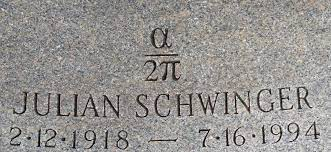
\includegraphics[]{images_ch5/schwinger_gravestone.jpeg}\\  Boston, lapide della tomba di \href{https://it.wikipedia.org/wiki/Julian_Schwinger}{Julian Schwinger}, premio Nobel insieme a Feynman e Tomonaga per gli studi sulla QED, uno fra tanti la sua rinormalizzazione al prim'ordine.}

Un risultato che, per essere compreso appieno, necessita di una piccola introduzione.

\subsection{Momento giromagnetico dell'elettrone}

\begin{definition}
    \textbf{(Momento Magnetico.)}
    
    Consideriamo una corrente planare di modulo $I$, che racchiude una superficie di area $S$ tale che \(\Vec{S} = S\hat{n}\), come in figura a lato.
    
    Si definisce momento magnetico il vettore 
    \begin{equation}
        \Vec{\mu} = I\Vec{S}
        \label{eq:magn_moment}
    \end{equation}
    Perpendicolare rispetto alla spira percorsa dalla corrente, secondo la regola della mano destra.
\end{definition}
\marginnote{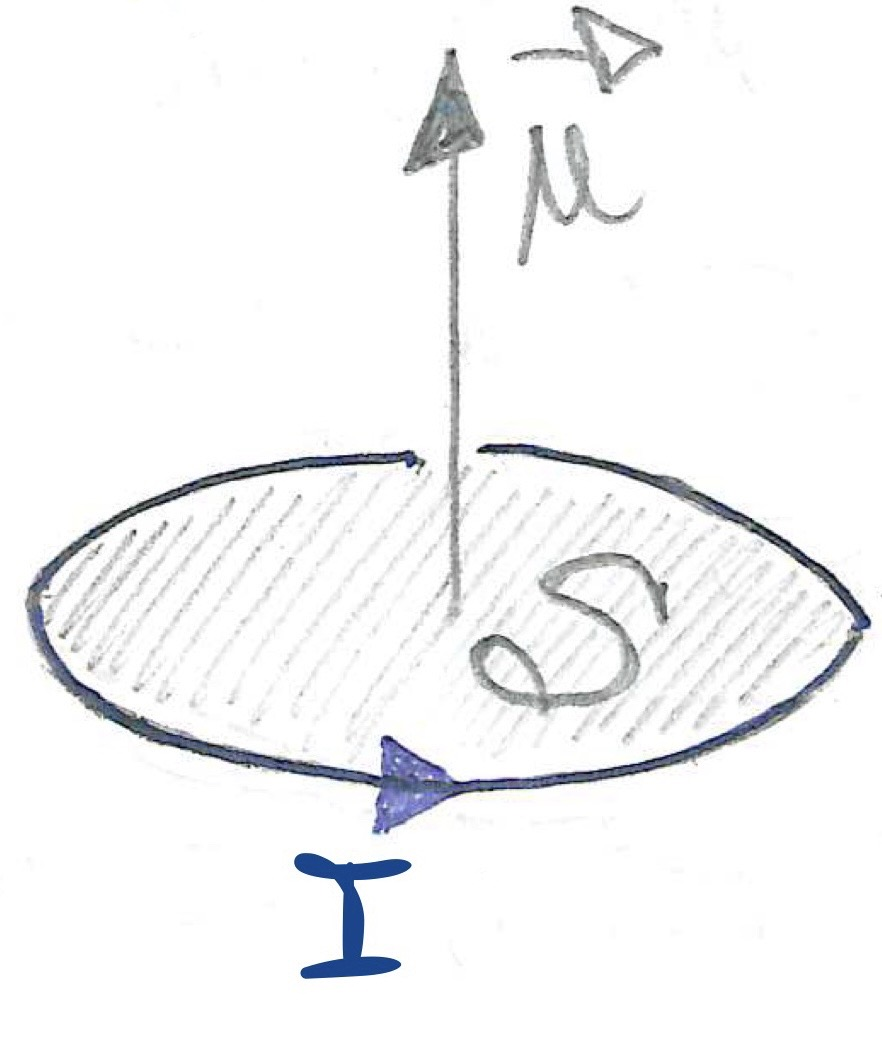
\includegraphics[]{images_ch5/magn_mom.jpg}} 

In presenza di un campo magnetico $\Vec{B}$, una spira subisce una coppia data da \(\Vec\tau = \Vec\mu \times \Vec{B} \), e si sviluppa un'energia potenziale associata alla direzione della spira rispetto al campo magnetico, i.e.:
\begin{equation}
    \boxed{U = -\Vec\mu\cdot\Vec{B}}
    \label{eq:potential_energy_magn_mom}
\end{equation}

La configurazione con \(\Vec{\mu}\parallel\Vec{B}\) coincide con la configurazione ad energia potenziale minore.

Consideriamo ora il caso in cui la corrente $I$ è generata da una carica $q$ che si muove nella spira con velocità angolare $\omega$. Tale corrente è esprimibile come segue:
\[
I = \frac{q}{T} = \frac{q\omega}{2\pi}
\]

Di conseguenza, assumendo la spira come circolare, con raggio $a$, abbiamo dalla sua definizione:
\[
\Vec\mu = \frac{q\omega}{2\pi}\pi a^2 \hat{n} = \frac{q}{2m} (\omega m a^2) \hat{n} = \frac{q}{2m}\Vec{L}
\]
dove abbiamo introdotto il momento angolare \(\Vec{L}=(\omega m a^2) \hat{n}\).

Quindi abbiamo:
\[
\boxed{\Vec\mu = \frac{q}{2m}\Vec{L} \quad ; \quad U = -\frac{q}{2m}\Vec{L}\cdot\Vec{B}}
\]

Classicamente, il momento magnetico è proporzionale al momento angolare delle particelle cariche. In meccanica quantistica, questa relazione si generalizza con la presenza dello spin.

Prendendo ad esempio un elettrone a riposo, il momento di dipolo magnetico è fornito dalla relazione:
\begin{equation}
    \boxed{\Vec\mu_e = \frac{-ge}{2m}\Vec{S}}
    \label{eq:electrone_dipole_moment}
\end{equation}
dove $\Vec{S}$ è l'operatore di spin, mentre $g$ è detto \textbf{momento giromagnetico dell'elettrone}.

Inoltre, l'Hamiltoniana di interazione in presenza di un campo magnetico esterno è
\begin{equation}
    \boxed{H_\text{int} = +\frac{ge}{2m}\Vec{S}\cdot\Vec{B}}
    \label{eq:magn_inter_hamiltonian}
\end{equation}

\subsection{Predizione di $g$ in QED}{
Vogliamo calcolare il valore del momento giromagnetico dell'elettrone in QED al tree-level. per farlo partiamo nuovamente dallo scattering Coulombiano in presenza di un potenziale esterno statico
\[
\feynmandiagram[vertical'=a to b] {
    i1 -- [fermion, edge label'=\(p\)] a[small, dot] -- [fermion, edge label'=\(p'\)] i2,
    b[large, crossed dot, label=right:\(A_\mu^{\text{ext}}(\Vec{x})\)] -- [photon, momentum'=\(q\)] a,
    };
\]
con \(q=p'-p\).

Come già argomentato all'inizio di questo capitolo, si trova:
\[
S_{fi} = (2\pi)\delta(E_{p'}-E_p)(ie)\bar u(p',s)\gamma^\mu u(p,r)A_\mu^{\text{ext}}(\Vec{q})
\]
La differenza rispetto a quanto già visto sta nel fatto che ora associamo ad \(A^\mu\) il 4-potenziale elettromagnetico dovuto ad un campo magnetico, i.e. 
\[
\begin{cases}
A^0=0\\
\Vec{B}=\Vec\nabla\times\Vec{A}
\end{cases}
\] 
In questo caso, la parte dell'ampiezza che sopravvive è quella che concerne la corrente spaziale, ovvero:
\[
\boxed{S_{fi} = (2\pi)\delta(E_{p'}-E_p)(ie)\bar u(p',s)\gamma^i u(p,r)A_i^{\text{ext}}(\Vec{q})}
\]

Ora valutiamone il limite non relativistico, lavorando al primo ordine in \(\Vec{q}\) e imponendo \(\Vec{p}=0\) in modo da poterci concentrare sullo spin.

La cinematica è quindi descritta da:
\[
p^\mu = \big(m, -\nicefrac{\Vec{q}}{2}\big) \quad p'^\mu = \big(m, \nicefrac{\Vec{q}}{2}\big)
\]
mentre possiamo esprimere gli spinori come segue:
\[
u(p,s) = \bigg(\frac{E+m}{2m}\bigg)^{\nicefrac{1}{2}}
\begin{pmatrix} 
\chi(s)\\
\frac{\Vec\sigma\cdot\Vec p}{E+m}\chi(s)
\end{pmatrix}\rightarrow
\begin{pmatrix} 
\chi(s)\\
\frac{-\Vec\sigma\cdot\Vec q}{4m}\chi(s)
\end{pmatrix}
\]

Adesso dobbiamo calcolare esplicitamente la corrente \( u^\dagger(p',s)\gamma^0 \gamma^i u(p,r)\).

Con la notazione di Dirac, abbiamo innanzitutto:
\[
\gamma^0\gamma^i = 
\begin{pmatrix}
    \mathbb 1   &   0\\
            0   &   - \mathbb 1
\end{pmatrix}
\begin{pmatrix}
            0   &   \sigma^i\\
    -\sigma^i   &   0
\end{pmatrix}
=
\begin{pmatrix}
            0   &   \sigma^i\\
    \sigma^i   &   0
\end{pmatrix}
\]
Di conseguenza:
\begin{align*}
    u^\dagger(p',s)\gamma^0 \gamma^i u(p,r) 
    &= 
    \begin{pmatrix} 
        \chi^\dagger(s) & \frac{\Vec\sigma\cdot\Vec q}{4m}\chi^\dagger(s)
    \end{pmatrix}
    \begin{pmatrix} 
        -\sigma^i\frac{\Vec\sigma\cdot\Vec q}{4m}\chi(r)\\
        \sigma^i\chi(r)
    \end{pmatrix}\\
    &=-\frac{1}{4m}\chi^\dagger(s) \big[\sigma^i (\Vec\sigma\cdot\Vec q)\big] \chi(r) + \frac{1}{4m}\chi^\dagger(s) \big[(\Vec\sigma\cdot\Vec q) \sigma^i\big] \chi(r)\\
    &=\frac{1}{4m}\chi^\dagger(s) \big[\sigma^j \sigma^i - \sigma^i \sigma^j\big]q^j \ \chi(r)
\end{align*}
Ricordiamo a questo punto le relazioni di commutazione tra le matrici di Pauli:
\(\big[\sigma^j, \sigma^i\big] = 2i\epsilon^{jik}\sigma^k\) e con un un paio di ulteriori manipolazioni (tra cui in particolare \(\epsilon^{jik} = -\epsilon^{ijk}\)) arriviamo al risultato finale:
\marginnote{Ricordiamo che $S^k$ è l'operatore di spin per il campo di Dirac.}
\begin{equation}
    \bar u(p',s)\gamma^i u(p,r) = \frac{-i}{m}\epsilon^{ijk}q^j \underbrace{\chi^\dagger(s)\frac{\sigma^k}{2}\chi(r)}_{\equiv \langle s|S^k|r\rangle}
    \label{eq:spatial_current}
\end{equation}

Ora possiamo sostituire la corrente nell'espressione per l'ampiezza, riscrivendola come segue:
\marginnote{Risulta utile riscrivere la parte spaziale del 4-potenziale in forma controvariante \(A_i\rightarrow A^i\), il che comporta un cambio di segno cancellato dalla permutazione del simbolo di Levi-Civita \(\epsilon^{ijk}\rightarrow-\epsilon^{kji}\), in modo da poter inserire nell'equazione il campo magnetico.}
\begin{align*}
    S_{fi} &\overset{\text{NR}}{=} (2\pi)\delta(E_{p'}-E_p)(ie)\Big[\frac{-i}{m}\epsilon^{ijk}q^j\langle s|S^k|r\rangle \Big]A_i^\text{ext}(\Vec{q})\\
    &= (2\pi)\delta(E_{p'}-E_p)\Big[\frac{e}{m} \textcolor{Green}{\epsilon^{kji}q^j} \langle s|S^k|r\rangle \Big]\textcolor{Green}{A^{\text{ext},i}(\Vec{q})}
\end{align*}

Ricordiamo che la relazione \(\Vec{B}=\Vec\nabla\times\Vec{A}\) si traduce in \(B^k = \epsilon^{kji}\partial_j A^i\), che nello spazio di Fourier diventa \(B^k = \epsilon^{kji}iq^jA^i\), da cui
\[
{-iB^k} = \textcolor{Green}{\epsilon^{kji}q^jA^i}
\]

Abbiamo quindi finalmente l'ampiezza in QED che cercavamo:
\marginnote{È interessante notare come l'equazione (\ref{eq:CoulombQEDamplitude_NR_treelevel}) ci stia dicendo che per mezzo dell'interazione con il campo magnetico si possono avere transizioni di spin!}
\begin{equation}
    \boxed{S_{fi} \overset{\text{NR}}{=} (2\pi)\delta(E_{p'}-E_p)\Big[\frac{(-ie)}{m}B^k\langle s|S^k|r\rangle\Big]}
    \label{eq:CoulombQEDamplitude_NR_treelevel}
\end{equation}

A questo punto compariamo quanto appena trovato con l'ampiezza calcolata in meccanica quantistica, utilizzando l'operatore (\ref{eq:magn_inter_hamiltonian})
\[
H_\text{int} = \frac{ge}{2m}\Vec{S}\cdot\Vec{B} =  \frac{ge}{2m}S^kB^k
\]

Abbiamo 
\begin{equation}
    \begin{aligned}
        A\big(|s\rangle\rightarrow|r\rangle\big) &= (2\pi)\delta(E_{p'}-E_p) (-i)\langle s|H_\text{int}|r\rangle \\
        & = (2\pi)\delta(E_{p'}-E_p) \frac{g(-ie)}{2m}\langle s|S^k|r\rangle B^k
    \end{aligned}
    \label{eq:CoulombQMamplitude_NR_treelevel}
\end{equation}
È evidente che il momento giromagnetico dell'elettrone, al tree-level, debba essere 
\begin{equation}
    \boxed{g=2}
    \label{eq:electr_gyromagn_factor_treelevel}
\end{equation}}

\subsection{$g$ oltre il tree level}
Includiamo le correzioni al loop nel calcolo fatto in sezione precedente, in particolare le correzioni al vertice, i.e.:
\[
 \bar u(p',s)\big(ie\gamma^\mu\big) u(p,r) \rightarrow \bar u(p',s)ie\Gamma^\mu(p',p) u(p,r)
\]
con, dalla (\ref{eq:vertex_formfactors}): \(\Gamma^\mu(p',p) = F_1(q^2)\gamma^\mu +\frac{i\sigma^{\mu\nu}q_\nu}{2m} F_2(q^2)\).

Dopo il processo di rinormalizzazione (in cui viene cancellato il termine UV-divergente \(F_{1,\text{1-loop}}(0)\) per mezzo del contro-termine \(\delta_1\)) il fattore di forma elettrico ha la seguente struttura:
\[
F_1(q^2) \approx 1+\frac{dF_{1,\text{1-loop}}(q^2)}{dq^2}\bigg|_{q^2=0}q^2 +\cdots
\]
Nel paragrafo precedente ci siamo limitati al tree-level, \(F_1(q^2) = 1\), e abbiamo detto di voler lavorare al prim'ordine in $q$. Di conseguenza, introducendo correzioni al loop non abbiamo bisogno di aggiungere termini dipendenti da \(F_1\) e possiamo concentrarci su \(F_2\):
\[
\boxed{\Gamma^\mu\rightarrow\frac{i\sigma^{\mu\nu}q_\nu}{2m}F_2(q^2=0) \quad , \quad q_\mu=(0,\Vec{q})}
\]

In termini di ampiezza di scattering, la correzione da calcolare è, trascurando il fattore \(2\pi\delta(E_{p'}-E_p)\):
\[
{\Delta S_{fi} = (ie)\bar u(p',s) \frac{i\sigma^{\mu\nu}q_\nu}{2m}F_2(q^2=0) u(p,r)A_\mu^\text{ext}(\Vec{q})} \quad , \quad A_\mu = (0,\Vec{A})
\]
di cui sopravvive solo la parte spaziale, che riportiamo utilizzando la notazione controvariante sia per l'impulso che per il potenziale (abbiamo due segni “$-$” che si elidono a vicenda): 

\begin{equation}
    \boxed{\Delta S_{fi} = \frac{(ie)}{2m}\bar u(p',s) i\sigma^{ij}q^j F_2(q^2=0) u(p,r)A^i}
    \label{eq:Sficorrection_start}
\end{equation}

Calcoliamo esplicitamente il prodotto spinoriale, utilizzando per prima cosa il commutatore tra le gamma di Dirac, con cui si identificano le matrici di Pauli in forma relativistica, \(\sigma_{\mu\nu} = \frac{i}{2}\big[\gamma_\mu,\gamma_\nu\big] \) e sostituendo le gamma stese in notazione di Dirac:
\begin{align*}
    \bar u(p',s) \sigma^{ij} u(p,r) &= \bar u(p',s) \frac{i}{2}\big(\gamma^i\gamma^j-\gamma^j\gamma^i\big) u(p,r) \\
    & = \frac{i}{2}\bar u(p',s) 
    \Bigg[
    \begin{pmatrix}
                0   &   \sigma^i \\
        -\sigma^i   &   0
    \end{pmatrix}
    \begin{pmatrix}
                0   &   \sigma^j \\
        -\sigma^j   &   0
    \end{pmatrix}
    -
    \begin{pmatrix}
                0   &   \sigma^j \\
        -\sigma^j   &   0
    \end{pmatrix}
    \begin{pmatrix}
                0   &   \sigma^i \\
        -\sigma^i   &   0
    \end{pmatrix}
    \Bigg] u(p,r)\\
    & = \frac{i}{2}\bar u(p',s) 
    \begin{pmatrix}
        -\sigma^i\sigma^j +\sigma^j\sigma^i  &   0 \\
        0   &  -\sigma^i\sigma^j +\sigma^j\sigma^i
    \end{pmatrix}u(p,r) \overset{\star}{=}
\end{align*}
Sulla diagonale riconosciamo il commutatore tra matrici di Pauli: \(\big[\sigma^j,\sigma^i\big]=2i\epsilon^{jik}\sigma^k\).

Inoltre, come già ribadito, vogliamo mantenere il calcolo al prim'ordine in $q$, quindi, data la presenza di $q^j$ in \(\Delta S_{fi}\), possiamo trascurare la parte proporzionale a $q$ nell'espressione dello spinore, i.e. prendiamo:
\[
u(p,s) = 
\begin{pmatrix}
    \chi(s)\\
    0
\end{pmatrix}
\]
Questo significa che possiamo trascurare la seconda riga della matrice al centro, in quanto il suo contributo verrà annullato dal prodotto con gli spinori.

In sostanza, otteniamo:
\begin{align*}
    \overset{\star}{=} \frac{i}{2}\chi^\dagger(s)\big( 2i\epsilon^{jik}\sigma^k \big) \chi(r) = -2\epsilon^{jik}\chi^\dagger(s) \frac{\sigma^k}{2} \chi(r) = -2\epsilon^{jik}\langle s | S^k | r \rangle
\end{align*}

Riassumendo:
\begin{equation}
    \boxed{\bar u(p',s) \sigma^{ij} u(p,r) = -2\epsilon^{jik}\langle s | S^k | r \rangle}
    \label{eq:current_correction}
\end{equation}

Sostituiamo quindi la (\ref{eq:current_correction}) nella (\ref{eq:Sficorrection_start}) e troviamo:
\begin{align*}
    \Delta S_{fi} = -\frac{e}{2m} q^j F_2(q^2=0) A^i \big[(-2)\epsilon^{jik}\langle s | S^k | r \rangle\big]
\end{align*}
Permutiamo gli indici del simbolo di Levi-Civita \(\epsilon^{jik}\rightarrow\epsilon^{kji}\) (questa volta la permutazione è pari, quindi non produce nessun “$-$”) e ritroviamo l'espressione del campo magnetico \(-iB^k = \epsilon^{kji}q^jA^i\).
Quindi troviamo:
\begin{equation}
    \boxed{\Delta S_{fi} = \frac{-ie}{m} F_2(q^2=0)  B^k\langle s | S^k | r \rangle}
    \label{eq:Sficorrection_end}
\end{equation}

Possiamo allora scrivere \textbf{l'ampiezza totale}:
\begin{equation}
    \boxed{S_{fi} + \Delta S_{fi} = (2\pi)\delta(E_{p'}-E_p)\frac{-ie}{2m}\Big[ 2 + 2F_2(q^2=0) \Big] B^k\langle s | S^k | r \rangle}
    \label{eq:Sfi_total}
\end{equation}
Non ci resta che comparare la (\ref{eq:Sfi_total}) con la (\ref{eq:CoulombQMamplitude_NR_treelevel}). Imponendo il loro rapporto = 1, troviamo la predizione per il \textbf{fattore giromagnetico dell'elettrone ad un loop}, i.e."
\begin{equation}
    \boxed{g=2\big[1 + F_{2,\text{1-loop}}(q^2=0)\big]}\quad , \text{con } F_{2,\text{1-loop}}(q^2=0) \overset{\ref{eq:F2_q0}}{=} \frac{\alpha}{2\pi}
\end{equation}

Possiamo andare oltre: esplicitando il valore del fattore di forma magnetico troviamo \(g=2+\nicefrac{\alpha}{\pi}\); inoltre possiamo dare la seguente definizione:
\begin{definition}
    \textbf{(Momento di dipolo magnetico anomalo dell'elettrone.)}

    Sia $g$ il fattore giromagnetico dell'elettrone a qualunque ordine, si definisce momento magnetico anomalo (di dipolo) il fattore:
    \begin{equation}
        a_e\equiv\frac{g-2}{2} \xrightarrow[]{\substack{\text{@ 1-loop}\\\text{in QED}}} a_e=\frac{\alpha}{2\pi}
        \label{eq:anomalous_magn_mom}
    \end{equation}
\end{definition}

\begin{nota}
    Abbiamo incluso solo un loop nel nostro calcolo. Tenere conto di correzioni con un numero di loop maggiore è piuttosto complesso se si vuole procedere analiticamente, in quanto il numero di diagrammi cresce esponenzialmente all'aumentare del numero di loop considerati.
    
    Inoltre, quando il numero di loop diventa sufficientemente elevato, andrebbe tenuto conto anche delle interazioni forti e deboli, dato che i fotoni possono interagire sia con gli adroni che con i \(W^\pm\).
    
    Ciò nonostante, persone con molta pazienza, tanto tempo libero, poca sanità mentale o, forse, computer sufficientemente potenti hanno calcolato il momento magnetico anomalo per l'elettrone ed il muone fino all'ordine $\alpha^5$.
    
    D'altro canto, sperimentalmente conosciamo queste grandezze fisiche con un'enorme precisione:
    \[
    \begin{cases}
        a_e^\text{exp} = 0.00115965218073(28)\\
        a_\mu^\text{exp} = 0.00116592091(63)
    \end{cases}
    \]
    e c'è una piccola discrepanza nel caso del muone:
    \[
     a_\mu^\text{exp} -  a_\mu^\text{th} \approx(23\pm6) \times 10^{-10}
    \]
    Questa discrepanza potrebbe dipendere da fisica oltre il modello standard, ma potrebbe anche dipendere da un piccolo errore teorico nella modellizzazione delle interazioni tra fotoni ed adroni.
\end{nota}


\section{Divergenze Infrarosse}
Lo studio delle divergenze infrarosse richiederebbe un corso a parte, in questa sezione vogliamo dare semplicemente alcune utili nozioni basilari.

Abbiamo già incontrato questo tipo di divergenze nel calcolo della derivata dell'auto-energia dell'elettrone nell'esercizio \ref{ex:dSigma_dpslashed}, così come anche nel calcolo del fattore di forma elettrico al loop in $q^2=0$, nell'esercizio \ref{ex:1loop_formfactor1}, e abbiamo visto che possono essere regolarizzate a patto dell'inserimento di una massa del fotone fittizia.

\subsection{Scattering Coulombiano al tree-level}
\marginnote{\[\feynmandiagram[horizontal'=a to b, inline=(a.base)] {
    i1 -- [anti fermion, edge label=\(p'\)] a[dot] -- [anti fermion, edge label=\(p\)] i2,
    b[large, crossed dot] -- [photon, momentum'=\(q\)] a
    };\]}
Studiamo nuovamente lo scattering Coulombiamo, di cui riportiamo la cinematica:
\[
\begin{aligned}
&p+q=p' \\
&E_p = E_{p'} \\\
&q^2=-|\Vec q|^2 = -2|\Vec p|^2\big(1-\cos\vartheta\big)
\end{aligned}
\Rightarrow
\begin{cases}
q = p' - p \\
|\Vec p| = |\Vec p'|\\
\boxed{q^2 = -4|\Vec p|^2 \sin^2\frac{\vartheta}{2}} 
\end{cases}
\]
Mentre per quanto riguarda l'ampiezza del processo al tree-level, abbiamo:
\[
\boxed{i\mathscr M_0  = (ie)\bar u (p',s)\gamma^0 u (p,r) \frac{Ze}{|\Vec{q}|^2}}
\]

Ne consegue che, ricordando quanto detto nella nota \ref{note:wick_contraction} in merito all'origine delle tracce e sfruttando le proprietà delle matrici $\gamma$:
\begin{align*}
    \frac{1}{2}\sum_{s,r}|\mathscr M_0|^2 &= \frac{Z^2e^4}{2|\Vec{q}|^4}\Tr{\big(\slashed p' + m\big)\gamma^0 \big(\slashed p + m\big)\gamma^0}\\
    &=\frac{Z^2e^4}{2|\Vec{q}|^4}4\big[2p^0p'^0 + m^2-p\cdot p'\big] \overset{\blacklozenge}{=}
\end{align*}
Adesso sostituiamo le condizioni cinematiche e semplifichiamo il semplificabile:

\begin{align*}
    \overset{\blacklozenge}{=}\frac{Z^2e^4}{8|\Vec p|^4 \sin^4\frac{\vartheta}{2}}\big[E^2 + m^2 + |\Vec{p}|^2 \cos\vartheta\big] 
\end{align*}
Si verifica che \(E^2 + m^2 + |\Vec{p}|^2 \cos\vartheta = 2E^2\big[ 1 - \beta^2\sin^2\frac{\vartheta}{2} \big]\) con \(\beta\equiv \frac{|\Vec{p}|}{E}\), quindi in definitiva:

\begin{align*}
\boxed{\frac{1}{2}\sum_{s,r}|\mathscr M_0|^2 = \frac{Z^2e^4}{4|\Vec p|^2\beta^2 \sin^4\frac{\vartheta}{2}}\bigg[ 1 - \beta^2\sin^2\frac{\vartheta}{2}\bigg]}
\end{align*}
Presa per nota la sezione d'urto differenziale \(\frac{d\sigma}{d\Omega}=\frac{1}{(4\pi)^2}\times \frac{1}{2}\sum_{s,r}|\mathscr M_0|^2\), abbiamo in questo caso:
\[
\frac{d\sigma}{d\Omega}= \frac{1}{2}\sum_{s,r}|\mathscr M_0|^2 = \frac{Z^2\alpha^2}{4|\Vec p|^2\beta^2 \sin^4\frac{\vartheta}{2}}\bigg[ 1 - \beta^2\sin^2\frac{\vartheta}{2}\bigg]
\]

\subsection{Correzioni al vertice}
Includiamo adesso le correzioni al vertice, studiando nuovamente il diagramma:
\marginnote{\(V\) sta ad identificare la presenza di un fotone Virtuale, e l'indice $\mu$ sarà contratto con la carica esterna che, come specificato nel seguito, al momento non abbiamo interesse a considerare.}
\[
\begin{tikzpicture}[baseline=\plusheight]
    \begin{feynman}
    \vertex (i) at (-2,1) {};
    \vertex[small, dot] (x) at (-1,0.5) {};
    \vertex[small, dot] (v) at (0,0) {};
    \vertex[small, dot] (y) at (1,0.5) {};
    \vertex (f) at (2,1) {};
    \vertex[large, crossed dot] (N) at (0,-1) {};
    \diagram*[small]{
    (i) --[fermion, edge label'=\(p\)] (x) --[fermion, edge label'=\(p-k\)] (v) --[fermion, edge label'=\(p'-k\)] (y) --[fermion, edge label'=\(p'\)] (f),
    (x) --[photon, half left, looseness=0.8, momentum=\(k\)](y),
    (N) --[photon] (v)
    };
    \end{feynman}
\end{tikzpicture} = i\mathscr M^\mu_V
\]
Abbiamo già studiato questo diagramma in precedenza, e abbiamo anche visto quanto fosse complesso il calcolo della sua ampiezza, da cui emergeva una divergenza infrarossa. 

L'idea è quella di svolgere nuovamente il calcolo di tale ampiezza, \textbf{tralasciando il potenziale generato dal nucleo}, utilizzando una serie di approssimazioni ad-hoc, utili ad isolare fin dal principio il termine divergente nel regime infrarosso.

In maniera preliminare scriviamo:
\begin{align*}
    i\mathscr M^\mu_V = i(ie)^3\int\frac{d^4k}{(2\pi)^4}\frac{1}{k^2+i\epsilon}\frac{\bar u(p')\gamma^\rho\big(\slashed p'-\slashed k + m\big)\gamma^\mu\big(\slashed p-\slashed k + m\big)\gamma_\rho u(p)}{\big[(p'-k)^2 -m^2 + i\epsilon\big]\big[(p-k)^2 -m^2 + i\epsilon\big]}
\end{align*}
$\blacktriangleright$ Siccome le divergenze IR appaiono nel limite \(\boxed{k\rightarrow0}\), questa sarà la nostra prima semplificazione: trascuriamo \(k\) al numeratore e \(k^2\) al denominatore; inoltre prendiamo i fermioni sulla shell di massa.
\begin{align*}
    i\mathscr M^\mu_V \overset{\text{IR}}{=} i(ie)^3\int\frac{d^4k}{(2\pi)^4}\frac{1}{k^2+i\epsilon}\frac{\bar u(p')\gamma^\rho\big(\slashed p' + m\big)\gamma^\mu\big(\slashed p+ m\big)\gamma_\rho u(p)}{\big[-2k\cdot p' + i\epsilon\big]\big[-2k\cdot p + i\epsilon\big]}
\end{align*}
$\blacktriangleright$ Ora semplifichiamo il numeratore per mezzo dell'equazione di Dirac:
\[
\begin{aligned}
    &\bar u(p') \big(\slashed p' - m\big) = 0  \\
    &\big(\slashed p - m\big)u(p) = 0
\end{aligned}
\Rightarrow
\begin{cases}
    \bar u(p') \slashed p' = \bar u(p')m \\
    \slashed p u(p)  =  m u(p)
\end{cases}
\]
Ma per farlo dobbiamo “girare” i prodotti \(\gamma^\rho \slashed p'\) e \(\slashed p\gamma_\rho\) sfruttando le relazioni di anticommutazione tra le gamma di Dirac \(\big[\gamma^\rho, \gamma^\mu\big]_+ = 2g^{\rho\mu}\).
\marginnote{
A titolo di esempio riportiamo l'operazione citata nel caso di $p'$:
\begin{align*}
    \gamma^\rho \slashed p' &= \gamma^\rho \gamma^\mu p'_\mu = (-\gamma^\mu\gamma^\rho + 2g^{\rho\mu})p'_\mu =\\
    &=-\slashed p'\gamma^\rho + 2p'^\rho 
\end{align*}}

Applicando questa operazione ed utilizzando successivamente \textcolor{blue}{l'equazione di Dirac} otteniamo:
\begin{align*}
    \mathscr N^\mu &= \bar u(p')\big(\Ccancel[blue]{-\slashed p'\gamma^\rho} + 2p'^\rho + \Ccancel[blue]{m\gamma^\rho}\big)\gamma^\mu\big(\Ccancel[blue]{-\gamma_\rho\slashed p} + 2p_\rho+ \Ccancel[blue]{\gamma_\rho m}\big) u(p)\\
    &=4p'\cdot p\,\bar u(p')\gamma^\mu u(p)
\end{align*}

Arriviamo quindi al seguente risultato

\begin{equation}
    \boxed{
    \begin{aligned}
        i\mathscr M^\mu_V \overset{\text{IR}}{=}&
        \bar u(p')\big(ie\gamma^\mu\big)u(p)\big(ie\big)^2 4ip'\cdot p\,\times \\
        &\times\int\frac{d^4k}{(2\pi)^4}\frac{1}{\big(k^2+i\epsilon\big)\big(2k\cdot p'-i\epsilon\big)\big(2k\cdot p-i\epsilon\big)}
    \end{aligned}}
    \label{eq:IR_factorized_coulomb_amplitude}
\end{equation}
Ci accorgiamo quindi del fatto che, nel limite infrarosso \(k\rightarrow0\), \textbf{la correzione virtuale} (dovuta allo scambio di un fotone virtuale tra le gambe esterne) \textbf{fattorizza nell'ampiezza al tree-level per un integrale IR-divergente}.

Diagrammaticamente: \marginnote{Notiamo come in questo passaggio il fattore 4 venga semplificato raccogliendo un 2 in ciascuna delle due parentesi a denominatore.}
\[
\boxed{
\begin{aligned}
    &\begin{tikzpicture}[baseline=\plusheight]
        \begin{feynman}
        \vertex (i) at (-1.5,1) {};
        \vertex[small, dot, Red] (x) at (-0.75,0.5) {};
        \vertex[small, dot, Red] (v) at (0,0) {};
        \vertex[small, dot, Red] (y) at (0.75,0.5) {};
        \vertex (f) at (1.5,1) {};
        \vertex (N) at (0,-1) {};
        \diagram*[small,Red]{
        (i) --[fermion, edge label'=\(p\)] (x) -- (v) -- (y) --[fermion, edge label'=\(p'\)] (f),
        (x) --[photon, half left, looseness=0.8](y),
        (N) --[photon] (v)
        };
        \end{feynman}
    \end{tikzpicture}\overset{\text{IR}}{=}
    \begin{tikzpicture}[baseline=\plusheight]
        \begin{feynman}
        \vertex (i) at (-1.5,1) {};
        \vertex[dot, Green] (v) at (0,0) {};
        \vertex (f) at (1.5,1) {};
        \vertex (N) at (0,-1) {};
        \diagram*[small,Green]{
        (i) --[fermion, edge label'=\(p\)] (v) --[fermion, edge label'=\(p'\)] (f),
        (N) --[photon] (v)
        };
        \end{feynman}
    \end{tikzpicture} \times \textcolor{blue}{\text{ Integrale IR-divergente}}\\
    &\textcolor{Red}{\mathscr M^\mu_V}\quad \overset{\text{IR}}{=}\quad \textcolor{Green}{\mathscr M_0^\mu} \quad\times\quad\textcolor{blue}{(-i)e^2 p\cdot p'\int\frac{d^4k}{(2\pi)^4}\frac{1}{\big(k^2+i\epsilon\big)\big(k\cdot p'-i\epsilon\big)\big(k\cdot p-i\epsilon\big)}}
\end{aligned}}
\]

Concentriamoci a questo punto sull'integrale su \(k\) e separiamo l'integrazione spaziale da quella temporale:
\[
\int\frac{d^3\Vec k}{(2\pi)^3}\int\limits_{-\infty}^{+\infty}\frac{d k^0}{(2\pi)}\frac{1}{\big[(k^0)^2-|\Vec{k}|^2+i\epsilon\big]}\frac{1}{\big(k^0p'^0 -\Vec{k}\cdot\Vec p' -i\epsilon\big)\big(k^0p^0 -\Vec{k}\cdot\Vec p-i\epsilon\big)} \overset{\star}{=}
\]
Consideriamo quindi i poli nel piano complesso di \(k^0\), e ci accorgiamo che tre dei poli si trovano sopra l'asse reale:
\marginnote{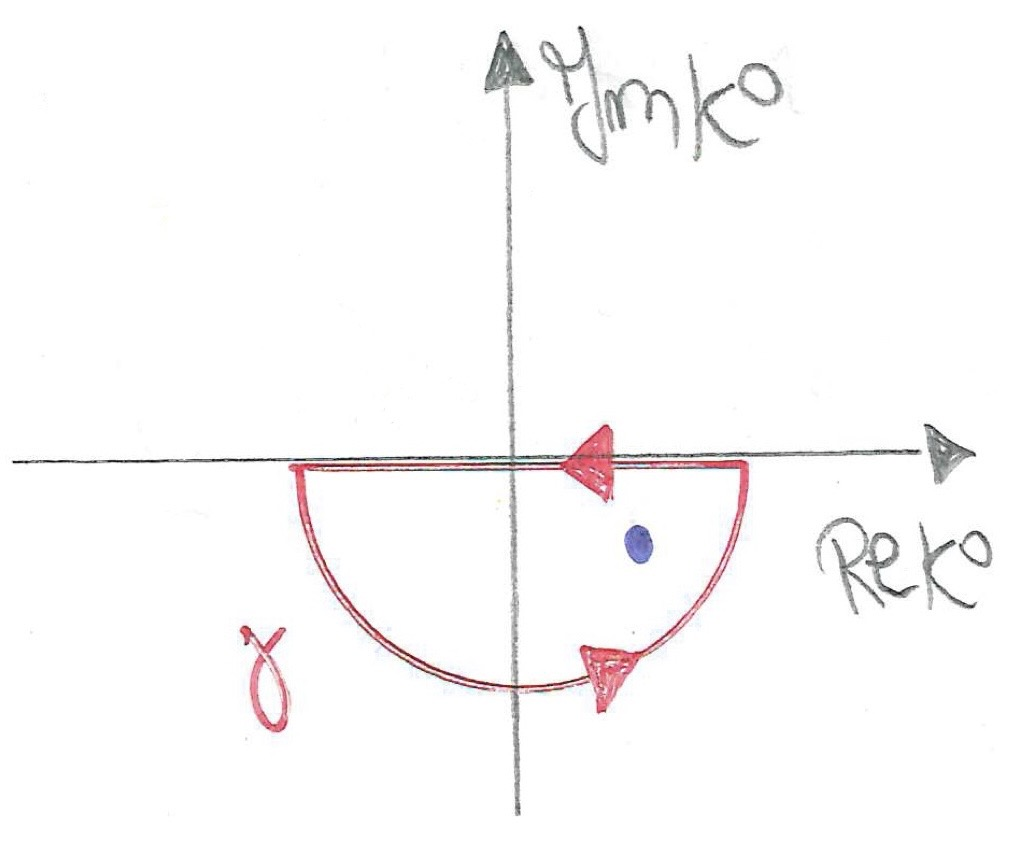
\includegraphics[]{images_ch5/k0_integration_contour.jpg}}
\[
k^0 =
\begin{cases}
      |\Vec{k}| - i\varepsilon\\ 
      -|\Vec{k}| + i\varepsilon
\end{cases} \quad , \quad
\begin{cases}
    k^0 = \frac{\Vec{k}\cdot\Vec p'}{p'^0} + i\varepsilon\\ \\
    k^0 = \frac{\Vec{k}\cdot\Vec p}{p^0} + i\varepsilon
\end{cases}
\]

Per comodità integriamo su una circonferenza nella parte inferiore del piano complesso come mostrato a lato, in modo da includere solo il polo \(k^0_\ast = |\Vec{k}| - i\varepsilon\).

Svolgendo il calcolo applicando il teorema dei residui e successivamente passando in coordinate polari modificando la misura di integrazione \(d^3\Vec k \rightarrow |\Vec{k}|^2 d|\Vec{k}|d\Omega\), otteniamo:

\[
\text{\marginnote{Ricordiamo che dal teorema dei residui, $\gamma$ come in figura, abbiamo (con il “$-$” per via del verso di integrazione):
\[\int_\gamma f(k^0) = - 2\pi i \text{Res}(f,k^0_\ast) \]
dove, per poli semplici come quello considerato:
\[
\text{Res}(f,k^0_\ast) = \lim_{k^0\rightarrow k^0_\ast}\big(k^0- k^0_\ast\big) f(k^0)
\]}}
\begin{aligned}
   &\overset{\star}{=}-i\int\frac{d^3\Vec k}{(2\pi)^3}\frac{1}{2|\Vec{k}|}\frac{1}{|\Vec{k}|^2\big(p'^0 -|\Vec{p}'| \cos\vartheta_{kp'}\big)\big(p^0 -|\Vec{p}| \cos\vartheta_{kp}\big)}\\
   &=-i \int\frac{\Ccancel[blue]{|\Vec{k}|^2} d|\Vec{k}|d\Omega}{(2\pi)^3 2|\Vec{k}|}\frac{1}{\Ccancel[blue]{|\Vec{k}|^2}\big(p'^0 -|\Vec{p}'| \cos\vartheta_{kp'}\big)\big(p^0 -|\Vec{p}| \cos\vartheta_{kp}\big)}
\end{aligned}
\]

In definitiva abbiamo l'espressione finale per la correzione virtuale:

\begin{equation}
    \boxed{
   \mathscr M^\mu_V \overset{\text{IR}}{=}\mathscr M_0^\mu
   \frac{(-e^2) p\cdot p'}{16\pi^3}\int \frac{d|\Vec{k}|}{|\Vec{k}|}\frac{d\Omega}{\big(p'^0 -|\Vec{p}'| \cos\vartheta_{kp'}\big)\big(p^0 -|\Vec{p}| \cos\vartheta_{kp}\big)}
   }
   \label{eq:IR_factorized_coulomb_amplitude_final}
\end{equation}
Questa ampiezza è, parlando in termini di power-counting, logaritmicamente divergente nel limite \(|\Vec{k}|\rightarrow 0\) (che corrisponde al limite \(\lambda \rightarrow\infty\)). Divergenze di questo tipo sono note come \textbf{divergenze infrarosse soft} o singolarità di massa (in quanto connesse alla presenza di particelle massless nello spettro).

\begin{nota}
    Consideriamo la parte angolare dell'integrale: i fattori \(\big(p'^0 -|\Vec{p}'| \cos\vartheta_{kp'}\big)\) e \(\big(p^0 -|\Vec{p}| \cos\vartheta_{kp}\big)\) non si annullano mai finché si considera l'elettrone come massivo.

    In realtà, se ci pensiamo su, in QED sono anche sempre strettamente positivi!
    Infatti la richiesta \(p^0 -|\Vec{p}| \cos\vartheta_{kp}<0\) richiederebbe 
    \[
    \cos\vartheta_{kp}>\frac{p^0}{|\Vec{p}|}
    \]
    ma l'energia dell'elettrone, a causa della sua massa, è sempre maggiore del modulo del suo impulso, seppure di poco, i.e.: \(\frac{p^0}{|\Vec{p}|} > 1\).

    Di conseguenza la condizione richiesta non può essere soddisfatta in alcun caso, e diciamo che \textbf{in QED con elettroni massivi sono presenti solo divergenze infrarosse soft legate al fotone massless}.
    \label{note:softIRdiv_are_related_to_photons_only}
\end{nota}
\begin{nota}
    Supponiamo per un attimo gli elettroni come particelle massless, i.e. \(p^0=|\Vec{p}|,~ p'^0=|\Vec{p'}|\). 

    In questo caso la funzione nell'integrale angolare diventa
    \[
    \frac{1}{|\Vec{p'}|\big(1- \cos\vartheta_{kp'}\big)|\Vec{p}|\big(1- \cos\vartheta_{kp}\big)}
    \]
    È evidente che questa funzione presenti divergenze nel limite \(\vartheta_{kp}\rightarrow 0\) oppure \(\vartheta_{kp'}\rightarrow 0\).

    Anche queste sono divergenze infrarosse, questa volta associate alla non-massività dell'elettrone, e sono dette \textbf{divergenze infrarosse collineari}. Ovviamente in massive-QED non avremo mai a che fare con questo tipo di divergenze, ma la situazione è diversa se si considerano altre teorie, come ad esempio la QCD.
    \label{note:collinear_IR_divergences}
\end{nota}

\subsection{Diagramma di emissione reale}
Fino ad ora abbiamo ragionato in termini di scattering Coulombiano, tuttavia il risultato che abbiamo ottenuto è piuttosto generale.

Consideriamo infatti il processo:
\[
e^-(p) + X \rightarrow e^-(p')+X
\]
che schematizziamo al tree-level (al solito indicato con il pedice “$0$”) come segue:
\[
\begin{tikzpicture}[baseline=\plusheight]
        \begin{feynman}
        \vertex (i) at (-1.5,1) {};
        \vertex[dot, fill=white!100, minimum size=7mm] (v) at (0,0) {\(iB\)};
        \vertex (f) at (1.5,1) {};
        \diagram*[small]{
        (i) --[fermion, edge label'=\(p\)] (v) --[fermion, edge label'=\(p'\)] (f),
        };
        \end{feynman}
    \end{tikzpicture}  \equiv i\mathscr M_0 = \bar u(p')iB u(p)
\]
dove \(iB\) rappresenta una generica interazione, ad esempio quella con una carica esterna nel caso dello scattering Coulombiano.

La sezione d'urto per questo processo sarà:
\[
\boxed{\sigma_0(e^-X\rightarrow e^-X) = \frac{1}{2\mathscr I}\int\sum_{s,r} |\mathscr M_0|^2d\Phi_{e^-X}}
\]
dove indichiamo con \(\mathscr I\) il flusso iniziale di elettroni e con \(d\Phi_{e^-X}\) l'elemento di spazio delle fasi su cui stiamo integrando per quanto riguarda lo stato finale.

Se adesso includiamo le correzioni al loop nella nostra trattazione e ripetiamo il calcolo fatto nel caso dello scattering Coulombiano, trascurando i termini di ordine \(k^2\) che emergono nei denominatori dei propagatori interni e semplificando il numeratore sfruttando l'equazione di Dirac, arriviamo anche in questo caso ad una fattorizzazione del tipo “ampiezza al tree-level $\times$ integrale IR-divergente”:

\[
\begin{tikzpicture}[baseline=\plusheight]
    \begin{feynman}
    \vertex (i) at (-1.5,1) {};
    \vertex[small, dot] (x) at (-0.75,0.5) {};
    \vertex[dot, fill=white!100, minimum size=7mm] (v) at (0,0) {\(iB\)};
    \vertex[small, dot] (y) at (0.75,0.5) {};
    \vertex (f) at (1.5,1) {};
    \vertex (N) at (0,-1) {};
    \diagram*[small]{
    (i) --[fermion, edge label'=\(p\)] (x) -- (v) -- (y) --[fermion, edge label'=\(p'\)] (f),
    (x) --[photon, half left, looseness=0.8](y),
    };
    \end{feynman}
\end{tikzpicture} = i\mathscr M_V \overset{\text{IR}}{=} i\mathscr M_0 \times \substack{\text{integrale} \\ \text{IR-divergente}}
\]

Il che ha senso se pensiamo al fatto che fotoni con lunghezze d'onda molto grandi sicuramente non saranno sensibili a processi di scattering che si svolgono a piccole scale, come il processo al tree-level.

Ora portiamo la discussione su questioni pratiche: il fatto che quest'ampiezza sia divergente è un bel problema. Infatti non c'è contro-termine che regga per regolarizzare questa divergenza, tutta la libertà che avevamo nel giocare con i parametri della teoria si è esaurita quando abbiamo rimosso le divergenze ultraviolette.

Nel momento in cui andiamo a calcolare la sezione d'urto ad un loop, fermandoci al prim'ordine in teoria delle perturbazioni (i.e. trascurando termini di ordine pari o superiore a \(|\mathscr M|^2\)), troviamo:
\begin{align*}
    \sigma_1(e^-X\rightarrow e^-X) &= \frac{1}{2\mathscr I}\int\sum_{s,r} |\mathscr M_0 + \mathscr M_V|^2 d\Phi_{e^-X}\\
    & = \frac{1}{2\mathscr I}\int\sum_{s,r}\Big[|\mathscr M_0|^2 + \mathscr M_0^\ast \mathscr M_V + \mathscr M_V^\ast \mathscr M_0\Big]\\
    & = \frac{1}{2\mathscr I}\int\sum_{s,r}|\mathscr M_0|^2 d\Phi_{e^-X} + \frac{1}{2\mathscr I}\int\sum_{s,r}\Big[ \mathscr M_0^\ast \mathscr M_V + \mathscr M_V^\ast \mathscr M_0\Big] d\Phi_{e^-X}
\end{align*}

Nel primo integrale riconosciamo la sezione d'urto al tree-level e se semplifichiamo il secondo a dovere il risultato finale sarà:
\begin{equation}
    \boxed{
    \begin{aligned}
        \sigma_1(e^-X\rightarrow e^-X) = ~
        &\sigma_0(e^-X\rightarrow e^-X) ~\times\\
        & \bigg[1 - \frac{e^2p\cdot p'}{8\pi^3}\int \frac{d|\Vec{k}|}{|\Vec{k}|}\frac{d\Omega}{\big(p'^0 -|\Vec{p}'| \cos\vartheta_{kp'}\big)\big(p^0 -|\Vec{p}| \cos\vartheta_{kp}\big)}\bigg]
    \end{aligned}
    }
    \label{eq:1loop_virtual_cross_section}
\end{equation}
Anche la sezione d'urto diverge nel limite infrarosso! Come facciamo ad eliminare queste divergenze senza usare i contro-termini?

L'idea è quella di considerare lo stesso processo includendo un fotone extra nello stato finale. Al tree-level questo significa considerare i diagrammi:

\[
\begin{tikzpicture}[baseline=\plusheight]
    \begin{feynman}
    \vertex (i) at (-1.5,1) {\(p\)};
    \vertex[small, dot] (x) at (-0.75,0.5) {};
    \vertex (z) at (0,1) {};
    \vertex[dot, fill=white!100, minimum size=7mm] (v) at (0,0) {\(iB\)};
    \vertex (f) at (1.5,1) {\(p'\)};
    \diagram*[small]{
    (i) --[fermion] (x) --[fermion, edge label'=\(p-k\)] (v) --[fermion] (f),
    (x) --[photon, momentum=\(k\)] (z),
    };
    \end{feynman}
\end{tikzpicture}
+
\begin{tikzpicture}[baseline=\plusheight]
    \begin{feynman}
    \vertex (i) at (-1.5,1) {\(p\)};
    \vertex (z) at (0.75,1.5) {};
    \vertex[dot, fill=white!100, minimum size=7mm] (v) at (0,0) {\(iB\)};
    \vertex[small, dot] (y) at (0.75,0.5) {};
    \vertex (f) at (1.5,1) {\(p'\)};
    \diagram*[small]{
    (i) --[fermion] (v) --[fermion, edge label'=\(p'+k\)] (y) --[fermion] (f),
    (y) --[photon, momentum=\(k\)] (z),
    };
    \end{feynman}
\end{tikzpicture}
\]
Il ragionamento per cui introduciamo questi diagrammi nel nostro calcolo regge anche dal punto di vista fisico: essendo l'elettrone una particella carica accelerata, deve perdere energia per irraggiamento!

Consideriamo il primo diagramma, la sua ampiezza (con il pedice $R$ ad indicare l'emissione di un fotone “Reale” e non virtuale) sarà:

\begin{align*}
    i\mathscr M_R^{(1)} &= \bar u(p')iB \frac{i\big(\slashed p - \slashed k + m\big)}{\big(p-k\big)^2 -m^2 + i\epsilon}\big[ie\gamma^\mu\varepsilon_\mu^\ast(k)\big]u(p) \\
    &\overset{\text{IR}}{=}\bar u(p')iB \frac{i\big(\slashed p + m\big)}{-2p\cdot k + i\epsilon}\big(ie\gamma^\mu\big)u(p)\varepsilon_\mu^\ast(k)\tikzmark{a}\\
    &=\bar u(p')iB \frac{(-e)2p^\mu\varepsilon_\mu^\ast(k)}{-2p\cdot k + i\epsilon}u(p) \tikzmark{b}\\
    &=\big[\bar u(p')iB u(p)\big]\frac{(-e)2p^\mu\varepsilon_\mu^\ast(k)}{-2p\cdot k + i\epsilon}
\end{align*}
\sidecomment{a}{b}{a}{eq. di Dirac}
E con le stesse modalità si trova l'espressione per il secondo diagramma. 

In sintesi abbiamo:
\begin{align*}
    &i\mathscr M_R^{(1)} \overset{\text{IR}}{=} i\mathscr M_0\bigg[\frac{(-e)2p^\mu\varepsilon_\mu^\ast(k)}{-2p\cdot k + i\epsilon}\bigg]\\
    &i\mathscr M_R^{(2)} \overset{\text{IR}}{=} i\mathscr M_0\bigg[\frac{(-e)2p'^\mu\varepsilon_\mu^\ast(k)}{2p'\cdot k + i\epsilon}\bigg]
\end{align*}

Di conseguenza possiamo scrivere l'ampiezza totale al tree-level:
\begin{equation}
    \boxed{
    i\mathscr M_R \overset{\text{IR}}{=} i\mathscr M_0\bigg[-e
    \underbrace{\bigg(\frac{2p'^\mu}{2p'\cdot k + i\epsilon} -\frac{2p^\mu}{2p\cdot k - i\epsilon}\bigg)}_{\substack{\text{fattori di emissione}\\\text{per un fotone soft}}}
    \varepsilon^\star_\mu(k)\bigg]}
    \label{eq:total_treelevel_amplitude_realemission}
\end{equation}

Non ci resta che calcolare la sezione d'urto, sommando su spin e polarizzazione dei fotoni nello stato finale e integrando sullo spazio delle fasi a tre corpi, ovvero:
\[
\sigma(e^-X\rightarrow e^-X+\gamma) = \frac{1}{2\mathscr I}\int\sum_{\text{spin}} |\mathscr M_R|^2d\Phi_{e^-X\gamma}
\]

Il risultato che otteniamo è il seguente:
\begin{equation}
    \boxed{
    \begin{aligned}
        \sigma(e^-X\rightarrow e^-X\gamma) \overset{\text{IR}}{=} ~
        &\sigma_0(e^-X\rightarrow e^-X) \sum_\text{elicità}\int \frac{d^3\Vec{k}}{(2\pi)^3 2E_k}e^2\Bigg\{ \\
        & \bigg(\frac{p'^\mu}{p'\cdot k}-\frac{p^\mu}{p\cdot k} \bigg) \varepsilon_\mu^\ast(k)\varepsilon_\nu(k) \bigg(\frac{p'^\nu}{p'\cdot k}-\frac{p^\nu}{p\cdot k}\bigg)\Bigg\}
    \end{aligned}
    }
    \label{eq:cross_section_total_realemission}
\end{equation}
Notiamo quindi due cose:
\begin{enumerate}
    \item[\textbf{i)}] Nel limite infrarosso lo spazio delle fasi fattorizza; infatti la parte che si riferisce allo stato finale \(e^-X\) insieme al flusso iniziale e al modulo quadro dell'ampiezza al tree-level ricostruiscono \(\sigma_0(e^-X\rightarrow e^-X)\).
    
    \item[\textbf{ii)}] La parte che descrive l'emissione del fotone genera invece un integrale su \(\Vec k\), sommato sulle polarizzazioni fisiche del fotone stesso.
\end{enumerate}
Concentriamoci sull'integrale di emissione: ricordando l'equazione (\ref{eq:polsum_final}) possiamo sostituire la somma sulle elicità dei vettori di polarizzazione con un tensore metrico con segno negativo, i.e. \(-g_{\mu\nu}\) (i termini aggiuntivi, come ampiamente discusso, sono irrilevanti). Gli indici degli impulsi sono quindi tutti uguali e possiamo svolgere i prodotti, ottenendo:
\[
-e^2\int \frac{d^3\Vec{k}}{(2\pi)^3 2|\Vec{k}|}\bigg[\frac{p'^2}{(p'\cdot k)^2} + \frac{p^2}{(p\cdot k)^2} -\frac{2p'\cdot p}{(p\cdot k)(p'\cdot k)}\bigg]
\]

Concentriamoci sul terzo termine, in quanto gli altri due vengono magicamente cancellati dal contro-termine \(\delta_2\).

Svolgiamo quindi il prodotto al denominatore e passiamo in coordinate polari:

\begin{align*}
    \frac{e^2(p\cdot p')}{8\pi^3}\int \frac{d|\Vec{k}|}{|\Vec{k}|}|\Vec{k}|^2d\Omega \frac{1}{|\Vec{k}|^2(p'^0-|\Vec{p}|\cos\vartheta_{kp'})(p^0-|\Vec{p'}|\cos\vartheta_{kp})}
\end{align*}
Questo integrale ci risulta piuttosto familiare. In effetti è esattamente identico a quello che appare nella sezione d'urto che abbiamo trovato studiando il diagramma con il fotone virtuale tra le gambe esterne, i.e. quella in equazione (\ref{eq:1loop_virtual_cross_section})!

Ciò significa che, fidandoci del fatto che gli altri due termini si cancellino per i motivi di cui sopra, \textbf{la somma delle due sezioni d'urto}
\[
\boxed{\sigma_1(e^-X\rightarrow e^-X) + \sigma(e^-X\rightarrow e^-X\gamma)}
\]
\textbf{non diverge nel limite infrarosso}, i.e. è \textit{IR-finite}.

\begin{nota}
    Rimarchiamo i due concetti chiave appena appresi in termini leggermente diversi:
    \begin{enumerate}
        \item[\textbf{1)}] Le sezioni d'urto \textbf{esclusive}, i.e. del tipo \(\sigma(e^-X\rightarrow e^-X)\), soffrono delle divergenze infrarosse e non sono quantità osservabili.
        \item[\textbf{2)}] Le sezioni d'urto \textbf{inclusive}, i.e. del tipo \(\sigma(e^-X\rightarrow e^-X +\gamma 's)\), sono libere dalle divergenze infrarosse.
    \end{enumerate}
    \label{note:exclusive/inclusive_xsec_remarks}
\end{nota}

Ragioniamo ora dal punto di vista sperimentale:
in quale senso \(\sigma(e^-X\rightarrow e^-X)\), come rimarcato nella nota \ref{note:exclusive/inclusive_xsec_remarks}, non è una quantità fisicamente osservabile? E perché dovremmo includere fotoni extra?

In un esperimento realistico, non avremo mai a disposizione un detector talmente sensibile da rivelare un fotone con energia \(E_\gamma\) piccola a piacere; difatti, dobbiamo sempre tener conto di una soglia \(\omega_\text{thr} \leftrightarrow E_\text{thr}\) sotto la quale questo detector non vede nulla.

Seguendo questa logica, appare evidente come lo stato finale \(|e^-X\gamma\rangle\), nel momento in cui \(E_\gamma < E_\text{thr}\), venga “visto” dal detector semplicemente come lo stato \(|e^-X\rangle\).

In altre parole, \textbf{le sezioni d'urto fisicamente misurabili devono includere ogni possibile numero di fotoni di bassa energia non rivelabili}. Riassumendo in formule:
\[
\boxed{\sigma(e^-X\rightarrow e^-X)_\text{obs} = \sigma(e^-X\rightarrow e^-X) + \sigma(e^-X\rightarrow e^-X+\gamma_{E_\gamma < E_\text{thr}})}
\]

Illustriamo a questo punto come avviene il processo di cancellazione delle divergenze. 
Partiamo dalla sezione d'urto esclusiva, i.e. l'equazione (\ref{eq:1loop_virtual_cross_section}), che può essere approssimata con le modalità che abbiamo già incontrato, introducendo la massa fittizia del fotone come regolatore per la divergenza infrarossa:
\[
\sigma_1(e^-X\rightarrow e^-X) \approx \sigma_0(e^-X\rightarrow e^-X)~\times~\bigg[ 1-\frac{\alpha}{\pi} f_{IR}\log\frac{E_e}{m_\gamma}\bigg]
\]

D'altro canto possiamo fare la stessa cosa anche per la sezione d'urto inclusiva, i.e. l'equazione (\ref{eq:cross_section_total_realemission}), con una piccola differenza. Abbiamo infatti:
\[
\sigma(e^-X\rightarrow e^-X\gamma) \approx \sigma_0(e^-X\rightarrow e^-X)~\times~\frac{\alpha}{\pi} f_{IR}\log\frac{\omega_\text{thr}}{m_\gamma}
\]

Il gioco è fatto! Se consideriamo la somma tra la sezione d'urto inclusiva ed esclusiva, cioè quella osservabile, separando i logaritmi vediamo che il termine con la “massa” del fotone si cancella!

\begin{equation}
    \boxed{
    \sigma(e^-X\rightarrow e^-X)_\text{obs} = \sigma_0(e^-X\rightarrow e^-X)~\times~\bigg[ 1-\frac{\alpha}{\pi} f_{IR}\log\frac{E_e}{\omega_\text{thr}}\bigg]
    }
    \label{eq:explicit_observable_xsec}
\end{equation}
L'equazione (\ref{eq:explicit_observable_xsec}) è \textit{IR-finite} nel limite \(m_\gamma\rightarrow 0\) e dipende dalla soglia \(\omega_\text{thr}>0\) in un esperimento reale. 

\begin{nota}
    Un piccolo recap sulla cancellazione delle divergenze.
    \begin{enumerate}
        \item[\textbf{UV:}] Emergono perché integriamo su un loop ad energie molto elevate \textcolor{gray}{[i.e., distanze estremamente corte]}, il che presumibilmente ci porta ben oltre la validità di qualsivoglia teoria quantistica di campo. 

        Il problema viene risolto reinterpretando la teoria e sfruttando i parametri liberi per cancellare i termini divergenti, connettendo questi parametri con le quantità osservabili.\\
        
        \item[\textbf{IR:}] Qui siamo nel caso opposto. Queste divegenze, infatti, appaiono quando si considera il limite di energia estremamente piccola \textcolor{gray}{[i.e., distanza estremamente grande]}. 
        
        Per correggere questo problema ridefiniamo le osservabili stesse, in quanto divergenze di questo tipo sono connesse a qualcosa che un esperimento realistico non sarà mai in grado di osservare.
    \end{enumerate}
\end{nota}

\begin{exercise}
    Nello studiare l'integrale di emissione abbiamo trascurato due dei tre termini che emergono nello sviluppo dell'espressione esplicita, i.e.: 
    \[
    -e^2\int \frac{d^3\Vec{k}}{(2\pi)^3 2|\Vec{k}|}\bigg[\underbrace{\frac{p'^2}{(p'\cdot k)^2} + \frac{p^2}{(p\cdot k)^2}}_{(\star)} -\frac{2p'\cdot p}{(p\cdot k)(p'\cdot k)}\bigg]
    \]
    Calcolare i contributi dei termini \((\star)\). Divergono nel limite infrarosso?
    [\textbf{conti svolti Lezione 18 pag. 80÷82}]
\end{exercise}



\end{document}

% \begin{figure}[h]
%     \centering
%     \includegraphics{images/semplicementepanati.png}
%     \caption*{}
%     \label{fig:my_label}
% \end{figure}